\documentclass[11pt]{article}
\usepackage[a4paper,margin=1in]{geometry}
\usepackage{amsmath,amssymb,amsthm,booktabs,enumitem}
\usepackage{fontspec}
\usepackage{unicode-math}
\usepackage{tikz}
\usepackage{pgfplots}
\usepackage[hidelinks]{hyperref}

\usetikzlibrary{arrows.meta,positioning}
\pgfplotsset{compat=1.18}

\setmainfont{TeX Gyre Pagella}
\setmathfont{TeX Gyre Pagella Math}

\setlist[itemize]{leftmargin=*, itemsep=2pt, topsep=4pt}
\setlist[enumerate]{leftmargin=*, itemsep=2pt, topsep=4pt}

\theoremstyle{definition}
\newtheorem{example}{Example}[section]

\newcommand{\R}{\mathbb{R}}
\newcommand{\C}{\mathbb{C}}
\newcommand{\N}{\mathbb{N}}
\newcommand{\E}{\mathbb{E}}
\newcommand{\Var}{\operatorname{Var}}
\newcommand{\Cov}{\operatorname{Cov}}
\newcommand{\Corr}{\operatorname{Corr}}
\newcommand{\rank}{\operatorname{rank}}
\newcommand{\Span}{\operatorname{span}}
\newcommand{\diag}{\operatorname{diag}}
\newcommand{\sgn}{\operatorname{sgn}}
\newcommand{\trace}{\operatorname{tr}}

\title{\textbf{Comprehensive Quant Interview Guide}}
\author{}
\date{XeLaTeX Edition}

\begin{document}
\maketitle

This document is a compact but rigorous interview companion. Each section contains the definitions and formulas that are most often used in quant interviews, followed by worked examples with complete solutions. The emphasis is on tools that recur in trading, research, and mathematical finance interviews: linear algebra, analysis, combinatorics, and probability.

\tableofcontents
\newpage

\section{Linear Algebra}
Quant interviews use linear algebra for covariance matrices, regressions, factor models, optimization, and stability questions. The focus is usually on structure: what a matrix or operator can and cannot do.

\subsection{Systems, Rank, Determinants, and Inverses}
\textbf{Definitions and formulas.}
\begin{itemize}
    \item A \emph{permutation} of $\{1,\dots,n\}$ is a bijection $\sigma$. Its sign is $\sgn(\sigma)=(-1)^{\mathrm{inv}(\sigma)}$, where $\mathrm{inv}(\sigma)$ is the number of inversions. Every permutation decomposes into disjoint cycles and also into a product of transpositions. These signs are exactly the coefficients that appear in determinant expansions.
    \item A complex number has Cartesian and polar forms
    \[
        z=x+iy=r(\cos\theta+i\sin\theta)=re^{i\theta}, \qquad |z|=\sqrt{x^2+y^2}.
    \]
    De Moivre's formula gives $(re^{i\theta})^n=r^n e^{in\theta}$, and the $n$th roots of unity are $e^{2\pi i k/n}$ for $k=0,\dots,n-1$. These facts are useful whenever eigenvalues or characteristic roots are complex.
    \item A linear system is written $Ax=b$. It is consistent if and only if
    \[
        \rank(A)=\rank([A\mid b]).
    \]
    If this common rank equals the number of unknowns, the solution is unique. Otherwise,
    \[
        x=x_p+x_h,
    \]
    where $x_p$ is one particular solution and $x_h$ runs over the nullspace of $A$. Rank counts the number of independent constraints, so free variables appear exactly when the rank is too small.
    \item Elementary row operations preserve the solution set of a system, and Gaussian elimination reduces a system to echelon form. In practice this is the fastest way to detect pivots, free variables, and inconsistency.
    \item For an invertible square matrix,
    \[
        A^{-1}=\frac{1}{\det(A)}\operatorname{adj}(A), \qquad \det(AB)=\det(A)\det(B).
    \]
    Also, $A$ is invertible if and only if $\det(A)\neq 0$. Invertibility means every right-hand side $b$ has a unique solution to $Ax=b$.
    \item The determinant is multilinear in rows (or columns), alternates under row swaps, and measures signed volume. A zero determinant signals linear dependence of rows or columns.
    \item A useful rank inequality is
    \[
        \rank(AB) \le \min\{\rank(A),\rank(B)\}.
    \]
    Composition cannot create more independent directions than either map already had.
    \item Iterative solvers appear in numerical interviews. Writing $A=D+L+U$ gives the Jacobi iteration
    \[
        x^{(k+1)} = D^{-1}(b-(L+U)x^{(k)}),
    \]
    and Gauss--Seidel iteration
    \[
        x^{(k+1)} = (D+L)^{-1}(b-Ux^{(k)}).
    \]
    A sufficient condition for convergence is strict diagonal dominance. These methods trade exact elimination for repeated cheap updates.
\end{itemize}

\begin{example}[Consistency and general solution]
Solve the system
\[
\begin{aligned}
x+y+z&=1,\\
2x+2y+2z&=2,\\
x-y&=0.
\end{aligned}
\]
Determine whether the solution is unique.
\end{example}

\begin{proof}[Solution]
The second equation is just twice the first, so it contributes no new information. The third equation gives $x=y$. Substituting into the first equation yields
\[
2x+z=1.
\]
Let $z=t$. Then
\[
x=y=\frac{1-t}{2}, \qquad z=t.
\]
Therefore the solution set is
\[
\left\{\left(\frac{1-t}{2},\frac{1-t}{2},t\right): t\in\R\right\}.
\]
This matches the rank test: $\rank(A)=\rank([A\mid b])=2<3$, so the system is consistent but has infinitely many solutions.
\end{proof}

\begin{example}[Independence of shifted determinants, and where it must fail]
Let $E$ be the $3\times3$ identity. (a) Prove that $\det(X)$, $\det(X+E)$, $\det(X-E)$, viewed as functions on the space of complex $3\times3$ matrices, are linearly independent. (b) Prove there is an $m\in\N$ for which $\det(X-mE),\det(X-(m-1)E),\dots,\det(X+mE)$ (a run of $2m+1$ such functions) is linearly \emph{dependent}.
\end{example}

\begin{proof}[Solution]
\textbf{Key reduction.} For a $3\times3$ matrix $X$, expanding $\det(X-kE)$ as a polynomial in the scalar $k$ gives exactly (up to sign) the characteristic polynomial of $X$:
\[
\det(X-kE) = -k^3+\trace(X)\,k^2-p_2(X)\,k+\det(X),
\]
where $p_2(X)$ is the sum of the principal $2\times2$ minors of $X$. So each function $f_k(X):=\det(X-kE)$ is a fixed linear combination of the four functions $\{1,\ \trace(X),\ p_2(X),\ \det(X)\}$ — namely $f_k = -k^3\cdot1+k^2\cdot\trace(X)-k\cdot p_2(X)+1\cdot\det(X)$ — with coefficient vector $v_k=(-k^3,k^2,-k,1)\in\C^4$. Since $1,\trace,p_2,\det$ have different degrees in the entries of $X$, they are linearly independent functions; hence the functions $\{f_k\}$ are linearly (in)dependent exactly when their coefficient vectors $\{v_k\}$ are linearly (in)dependent in $\C^4$.

\textbf{(a)} Here $k\in\{-1,0,1\}$: $v_{-1}=(1,1,1,1)$, $v_0=(0,0,0,1)$, $v_1=(-1,1,-1,1)$. Suppose $\alpha v_{-1}+\beta v_0+\gamma v_1=0$. The third coordinate gives $\alpha-\gamma=0$, i.e.\ $\alpha=\gamma$; the second coordinate gives $\alpha+\gamma=0$, i.e.\ $\alpha=-\gamma$. Together $\alpha=\gamma=0$, and then the fourth coordinate gives $\beta=0$. So $v_{-1},v_0,v_1$ are linearly independent in $\C^4$, hence so are $f_{-1},f_0,f_1$:
\[
\boxed{\det(X),\ \det(X+E),\ \det(X-E) \text{ are linearly independent}}.
\]

\textbf{(b)} Since $\C^4$ is $4$-dimensional, any $5$ vectors in it are automatically linearly dependent. Taking $m=2$ gives $2m+1=5$ functions $f_{-2},f_{-1},f_0,f_1,f_2$, whose coefficient vectors $v_{-2},\dots,v_2\in\C^4$ (five vectors in a four-dimensional space) must be dependent, hence so are the functions themselves:
\[
\boxed{m=2 \text{ works: } \det(X-2E),\dots,\det(X+2E) \text{ are linearly dependent}}
\]
(indeed any $m\ge2$ works, by the same pigeonhole argument).
\end{proof}

\begin{example}[A rank-drop inequality for $A$ and $A^2$]
Let $A$ be an $n\times n$ matrix. Prove $n-\rank A \ge \rank A - \rank A^2$.
\end{example}

\begin{proof}[Solution]
Restrict $A$ to a map $\operatorname{im}(A)\to\R^n$. Its image is $A(\operatorname{im}A)=\operatorname{im}(A^2)$, and its kernel is $\ker(A)\cap\operatorname{im}(A)$. By rank–nullity applied to this restriction,
\[
\rank(A^2)=\dim\operatorname{im}(A^2) = \dim\operatorname{im}(A) - \dim\big(\ker(A)\cap\operatorname{im}(A)\big)
\]
\[
= \rank(A) - \dim\big(\ker(A)\cap\operatorname{im}(A)\big),
\]
so
\[
\rank(A)-\rank(A^2) = \dim\big(\ker(A)\cap\operatorname{im}(A)\big).
\]
Since $\ker(A)\cap\operatorname{im}(A)$ is a subspace of $\ker(A)$, its dimension is at most $\dim\ker(A) = n-\rank(A)$ (ordinary rank–nullity for $A$). Combining,
\[
\boxed{n-\rank(A) \ge \rank(A)-\rank(A^2)}.
\]
\end{proof}

\subsection{Vector Spaces and Linear Maps}
\textbf{Definitions and formulas.}
\begin{itemize}
    \item A set $V$ is a vector space if it is closed under addition and scalar multiplication. A \emph{basis} is a linearly independent spanning set. The number of basis vectors is $\dim(V)$. A basis is the coordinate system intrinsic to the space.
    \item For subspaces $U,V\subseteq \R^n$,
    \[
        \dim(U+V)=\dim(U)+\dim(V)-\dim(U\cap V).
    \]
    If $U\cap V=\{0\}$, then $U\oplus V$ is a direct sum and $\dim(U\oplus V)=\dim(U)+\dim(V)$. The overlap must be subtracted because it would otherwise be counted twice.
    \item If $L:V\to W$ is linear, then
    \[
        \ker(L)=\{v\in V:L(v)=0\}, \qquad \operatorname{im}(L)=\{L(v):v\in V\},
    \]
    and the rank--nullity theorem says
    \[
        \dim(\ker L)+\dim(\operatorname{im}L)=\dim(V).
    \]
    The kernel measures directions lost by the map, while the image measures directions that survive.
    \item If $C$ is the change-of-basis matrix from the new basis to the old one, then the matrix of an operator changes by similarity:
    \[
        A_{\text{new}}=C^{-1}A_{\text{old}}C.
    \]
    Similar matrices represent the same linear transformation in different coordinates.
    \item In regression and least squares,
    \[
        \min_x \|Ax-b\|_2^2
        \quad \Longrightarrow \quad
        A^TAx=A^Tb.
    \]
    The normal equations say that the residual $b-Ax$ must be orthogonal to the column space of $A$.
\end{itemize}

\begin{example}[Dimension of a constrained symmetric matrix space]
Let subspaces $V,U\subseteq \R^4$ be defined by
\[
V=\Span\{v_1,v_2,v_3\}, \qquad U=\{y\in\R^4:Ty=0\},
\]
where
\[
v_1=(3,-2,2,1)^T,\qquad
v_2=(-1,2,-2,3)^T,\qquad
v_3=(3,-3,-1,2)^T,
\]
and
\[
T=(2,-1,-3,-2).
\]
Define
\[
F=\left\{A\in M_4(\R): \text{every column of }A\text{ lies in }V,\ \text{every row of }A\text{ lies in }U\right\}.
\]
Find
\[
W=\{A\in M_4(\R): A=A^T,\ A\in F\}.
\]
Write an integer as the answer, or $-1$ if the set is not a linear space.
\end{example}

\begin{proof}[Solution]
The set $W$ is a linear subspace because symmetry and the row/column constraints are all linear conditions.

First compute the dimension of $V\cap U$.
\begin{itemize}
    \item The vectors $v_1,v_2,v_3$ are linearly independent, so $\dim(V)=3$.
    \item Since $U=\ker(T)$ with $T\neq 0$, we have $\dim(U)=3$.
    \item Now
    \[
        Tv_2 = 2(-1)-2+6-6 = -4 \neq 0,
    \]
    so $v_2\notin U$. Therefore $V$ is not contained in $U$, hence $V+U=\R^4$.
\end{itemize}
Therefore,
\[
\dim(V\cap U)=\dim(V)+\dim(U)-\dim(V+U)=3+3-4=2.
\]
Set $I=V\cap U$, so $\dim(I)=2$.

Now let $A\in W$. Since the columns of $A$ lie in $V$ and $A=A^T$, each row is the transpose of a column. Because each row lies in $U$, each column also lies in $U$. Thus every column of $A$ lies in $I=V\cap U$. So the image of $A$ is contained in the two-dimensional space $I$.

Because $A$ is symmetric, in an orthonormal basis adapted to the decomposition
\[
\R^4 = I \oplus I^\perp,
\]
the matrix of $A$ has block form
\[
\begin{pmatrix}
B & 0 \\
0 & 0
\end{pmatrix},
\]
where $B$ is a symmetric $2\times 2$ real matrix. The space of symmetric $2\times 2$ matrices has dimension
\[
\frac{2(2+1)}{2}=3.
\]
Hence
\[
\boxed{\dim(W)=3}.
\]
\end{proof}

\begin{example}[Least-squares solution via normal equations]
Find the least-squares solution of
\[
A x \approx b,
\qquad
A=
\begin{pmatrix}
1&1\\
1&-1\\
1&0
\end{pmatrix},
\qquad
b=
\begin{pmatrix}
1\\
0\\
2
\end{pmatrix}.
\]
\end{example}

\begin{proof}[Solution]
The least-squares solution satisfies the normal equations
\[
A^TAx=A^Tb.
\]
Compute
\[
A^TA=
\begin{pmatrix}
3&0\\
0&2
\end{pmatrix},
\qquad
A^Tb=
\begin{pmatrix}
3\\
1
\end{pmatrix}.
\]
Therefore
\[
\begin{pmatrix}
3&0\\
0&2
\end{pmatrix}
\begin{pmatrix}
x_1\\
x_2
\end{pmatrix}
=
\begin{pmatrix}
3\\
1
\end{pmatrix},
\]
so
\[
x_1=1,
\qquad
x_2=\frac12.
\]
Hence the least-squares solution is
\[
\boxed{x^*=\begin{pmatrix}1\\[2pt] \frac12\end{pmatrix}}.
\]
Indeed,
\[
Ax^*=
\begin{pmatrix}
3/2\\
1/2\\
1
\end{pmatrix},
\qquad
r=b-Ax^*=
\begin{pmatrix}
-1/2\\
-1/2\\
1
\end{pmatrix},
\]
and one checks that $r$ is orthogonal to both columns of $A$, as it should be.
\end{proof}

\begin{example}[Prescribing an eigenvector and excluding a vector from the image]
Let $v,w\in\R^n$ be linearly independent. Does there always exist an $n\times n$ matrix $A$ such that $v$ is an eigenvector of $A$ with eigenvalue $5$, while $w\notin \operatorname{im}(A)$?
\end{example}

\begin{proof}[Solution]
Yes, always. Since $v,w$ are linearly independent, extend $\{v,w\}$ to a basis $\{v,w,e_3,\dots,e_n\}$ of $\R^n$. A linear map is determined by its values on a basis, so define $A$ by
\[
Av=5v, \qquad Aw=0, \qquad Ae_3=\cdots=Ae_n=0.
\]
By construction $v$ is an eigenvector of $A$ with eigenvalue $5$. Moreover
\[
\operatorname{im}(A)=\Span\{5v,0,\dots,0\}=\Span\{v\},
\]
and $w\notin\Span\{v\}$ precisely because $v,w$ are linearly independent. Hence
\[
\boxed{w\notin \operatorname{im}(A)}
\]
for this choice of $A$. Concretely: writing any $x\in\R^n$ in basis coordinates $x=\alpha v+\beta w+\sum_i\gamma_ie_i$, one has $Ax=5\alpha v$.
\end{proof}

\begin{example}[Equal rank from an invertibility hypothesis]
Let $A,B$ be $n\times n$ matrices with $A^2=A$, $B^2=B$, and suppose $I-(A+B)$ is invertible. Prove that $\rank A=\rank B$.
\end{example}

\begin{proof}[Solution]
Let $C=I-A-B$, invertible by hypothesis. Since $A$ is idempotent, every $v\in\operatorname{im}(A)$ satisfies $Av=v$ (write $v=Au$; then $Av=A^2u=Au=v$), and likewise $Bv=v$ for $v\in\operatorname{im}(B)$.

Take $v\in\operatorname{im}(A)$. Then
\[
Cv=v-Av-Bv=v-v-Bv=-Bv\in\operatorname{im}(B),
\]
so $C$ maps $\operatorname{im}(A)$ into $\operatorname{im}(B)$. As $C$ is invertible it is injective, so its restriction to $\operatorname{im}(A)$ is an injective map into $\operatorname{im}(B)$, giving
\[
\rank A=\dim\operatorname{im}(A)\le \dim\operatorname{im}(B)=\rank B.
\]
Symmetrically, for $v\in\operatorname{im}(B)$,
\[
Cv=v-Av-Bv=v-Av-v=-Av\in\operatorname{im}(A),
\]
so the same argument gives $\rank B\le\rank A$. Combining,
\[
\boxed{\rank A=\rank B}.
\]
\end{proof}

\subsection{Eigenvalues, Jordan Form, and Singular Value Decomposition}
\textbf{Definitions and formulas.}
\begin{itemize}
    \item A scalar $\lambda$ is an eigenvalue of $A$ if there exists $v\neq 0$ such that $Av=\lambda v$. The eigenspace is $E_\lambda=\ker(A-\lambda I)$. Eigenvectors are directions whose orientation is preserved by the transformation.
    \item The characteristic polynomial is $p_A(\lambda)=\det(\lambda I-A)$. The Hamilton--Cayley theorem states that $p_A(A)=0$. This lets you reduce high powers of a matrix to lower ones.
    \item For an $n\times n$ matrix, the sum of eigenvalues counted with algebraic multiplicity is $\trace(A)$ and the product is $\det(A)$. These are quick consistency checks when you compute a spectrum.
    \item A matrix is diagonalizable if and only if for every eigenvalue, algebraic multiplicity equals geometric multiplicity. Equivalently, the space has a full basis of eigenvectors.
    \item In particular, if the characteristic polynomial splits and has distinct roots, the matrix is automatically diagonalizable. Distinct eigenvalues automatically give linearly independent eigenvectors.
    \item A nilpotent operator satisfies $N^k=0$ for some $k$. Its Jordan form is a direct sum of Jordan blocks with zero diagonal. Nilpotent parts measure failure of diagonalizability.
    \item If $N$ is nilpotent on an $n$-dimensional space, then its only eigenvalue is $0$ and its characteristic polynomial is $\lambda^n$. Repeated application eventually kills every vector.
    \item The singular value decomposition is
    \[
        A=U\Sigma V^T,
    \]
    where $U,V$ are orthogonal and $\Sigma$ is diagonal with nonnegative entries $\sigma_i=\sqrt{\lambda_i(A^TA)}$. The SVD separates input directions, stretching factors, and output directions.
    \item The singular values measure the principal stretching factors of the linear map $x\mapsto Ax$. The rank of $A$ equals the number of nonzero singular values. For rectangular matrices they play the role that absolute eigenvalues play for symmetric matrices.
    \item If $A$ is real symmetric, then the spectral theorem gives
    \[
        A=Q\Lambda Q^T,
    \]
    where $Q$ is orthogonal and $\Lambda$ is diagonal with real eigenvalues. Symmetric matrices therefore act like independent scalar multipliers along orthogonal directions.
    \item The Frobenius norm is
    \[
        \|A\|_F=\sqrt{\trace(A^TA)}=\left(\sum_{i,j} a_{ij}^2\right)^{1/2}=\left(\sum_i \sigma_i^2\right)^{1/2}.
    \]
    It is the Euclidean norm of the matrix entries viewed as one long vector, and it is the natural norm for entrywise least-squares error.
    \item The best rank-$k$ approximation in Frobenius norm is obtained by truncating the SVD:
    \[
        A_k=\sum_{i=1}^k \sigma_i u_i v_i^T.
    \]
    Keeping the largest singular values preserves the most important directions of variation.
\end{itemize}

\begin{example}[Using Hamilton--Cayley to compute powers]
Let
\[
A=\begin{pmatrix}2&1\\0&2\end{pmatrix}.
\]
Find a formula for $A^n$.
\end{example}

\begin{proof}[Solution]
Write
\[
A=2I+N, \qquad N=\begin{pmatrix}0&1\\0&0\end{pmatrix}, \qquad N^2=0.
\]
Because $N^2=0$, the binomial expansion truncates:
\[
A^n=(2I+N)^n=\sum_{k=0}^n \binom{n}{k}2^{n-k}N^k = 2^n I + n2^{n-1}N.
\]
Hence
\[
A^n=
\begin{pmatrix}
2^n & n2^{n-1} \\
0 & 2^n
\end{pmatrix}.
\]
This is exactly what Hamilton--Cayley predicts, since the characteristic polynomial is $(\lambda-2)^2$ and therefore $(A-2I)^2=0$.
\end{proof}

\begin{example}[Singular values of a rank-one matrix]
Let
\[
A=\begin{pmatrix}3&0\\4&0\end{pmatrix}.
\]
Find the singular values of $A$ and write down one SVD.
\end{example}

\begin{proof}[Solution]
Compute
\[
A^TA=\begin{pmatrix}25&0\\0&0\end{pmatrix}.
\]
Its eigenvalues are $25$ and $0$, so the singular values are
\[
\sigma_1=5, \qquad \sigma_2=0.
\]
Take
\[
v_1=\begin{pmatrix}1\\0\end{pmatrix}, \qquad v_2=\begin{pmatrix}0\\1\end{pmatrix}.
\]
Then
\[
u_1=\frac{Av_1}{\|Av_1\|}=\frac{1}{5}\begin{pmatrix}3\\4\end{pmatrix}=
\begin{pmatrix}3/5\\4/5\end{pmatrix}.
\]
Choose an orthonormal vector perpendicular to $u_1$, for example
\[
u_2=\begin{pmatrix}-4/5\\3/5\end{pmatrix}.
\]
Therefore one valid SVD is
\[
U=\begin{pmatrix}3/5&-4/5\\4/5&3/5\end{pmatrix},
\qquad
\Sigma=\begin{pmatrix}5&0\\0&0\end{pmatrix},
\qquad
V=I.
\]
So
\[
\boxed{A=U\Sigma V^T}
\]
with singular values $5$ and $0$.
\end{proof}

\begin{example}[Centralizer dimension for cyclic vs.\ non-cyclic matrices]
For an $n\times n$ real matrix $A$ and $v\in\R^n$, let $U(A)=\{X\in\mathrm{Mat}_n(\R): AX=XA\}$ and $W(A,v)=\Span\{v,Av,A^2v,\dots\}$ (the $A$-cyclic subspace generated by $v$).
(a) If $\dim W(A,v)=n$ for \emph{every} $v\neq0$, what is the largest possible $\dim U(A)$?
(b) If $\dim W(A,v)<n$ for \emph{every} $v$, what is the smallest possible $\dim U(A)$?
\end{example}

\begin{proof}[Solution]
\textbf{Background fact.} For any $A$, $\dim U(A)\ge n$, with equality iff $A$ is \emph{non-derogatory} (its minimal polynomial has degree $n$, i.e.\ equals the characteristic polynomial). More precisely, if the Jordan blocks for a single eigenvalue have sizes $n_1\ge n_2\ge\cdots\ge n_r$ (a partition of that eigenvalue's multiplicity), that eigenvalue contributes $\sum_i (2i-1)n_i$ to $\dim U(A)$; summing over eigenvalues and minimizing $\sum(2i-1)n_i$ for fixed $\sum n_i$ shows single blocks ($r=1$) are optimal, giving the bound $\dim U(A)\ge n$.

\textbf{(a)} If $v_0$ is any vector with $\dim W(A,v_0)=n$, then $v_0,Av_0,\dots,A^{n-1}v_0$ are linearly independent, so the minimal polynomial of $A$ has degree $\ge n$, hence exactly $n$: $A$ is non-derogatory. By the background fact, $\dim U(A)=n$ exactly. So under the hypothesis of (a) (which certainly implies \emph{some} cyclic vector exists), the dimension is forced to be
\[
\boxed{n}.
\]
(Such $A$ exist for even $n$: e.g.\ for $n=2$, $A=\begin{pmatrix}0&-1\\1&0\end{pmatrix}$ has no real eigenvalues, so $\{v,Av\}$ is dependent only if $v$ is a real eigenvector — impossible — hence every nonzero $v$ is cyclic.)

\textbf{(b)} Now no vector is cyclic, so $A$ is derogatory: some eigenvalue has $r\ge2$ Jordan blocks. To minimize $\dim U(A)=\sum(2i-1)n_i$ (summed over all eigenvalues) subject to this, isolate the derogatory eigenvalue's contribution $n_1+3n_2$ with $n_1\ge n_2\ge1$: writing the eigenvalue's multiplicity as $m=n_1+n_2$, this equals $m+2n_2\ge m+2$, minimized at $n_2=1$ (a single ``stray'' Jordan block of size $1$ split off from an otherwise full block of size $n-1$). Every other eigenvalue, kept non-derogatory, contributes exactly its own multiplicity. Summing, the total is minimized at
\[
\boxed{n+2},
\]
attained by a single eigenvalue with Jordan blocks of sizes $(n-1,1)$.
\end{proof}

\begin{example}[When is a matrix forced to be invertible by $A^T=p(A)$?]
Let $A$ be a square real matrix with $A^T=p(A)$ for some polynomial $p$ with nonzero constant term. Prove $A$ is invertible. Is it true that for \emph{every} linear operator $\varphi:\R^n\to\R^n$ there is a polynomial $p$ and a basis in which the matrix of $\varphi$ satisfies $A^T=p(A)$ (dropping the nonzero-constant-term requirement)?
\end{example}

\begin{proof}[Solution]
\textbf{Invertibility.} Write $p(x)=c_0+c_1x+\cdots+c_kx^k$ with $c_0\neq0$. Suppose toward a contradiction that $A$ is singular, so $Av=0$ for some $v\neq0$. Then $A^jv=0$ for all $j\ge1$, so $p(A)v=c_0v$, i.e.\ $A^Tv=c_0v$. Now use the general identity $v^TAv=v^TA^Tv$ (true for any square matrix and vector, since $v^TAv$ is a scalar equal to its own transpose $v^TA^Tv$). The left side is $v^T(Av)=v^T\cdot 0=0$; the right side is $v^T(A^Tv)=v^T(c_0v)=c_0\|v\|^2$. So $c_0\|v\|^2=0$, and since $v\neq0$ this forces $c_0=0$ — contradicting $c_0\neq0$. Hence $A$ is invertible.

\textbf{Every operator?} No. If $A^T=p(A)$ for any polynomial $p$, then $A$ commutes with $A^T$ (it commutes with any polynomial in itself), so $A$ is a \emph{normal} matrix in that basis. Take $\varphi$ with matrix $A_0=\begin{pmatrix}0&1\\0&0\end{pmatrix}$ in the standard basis (a nonzero nilpotent operator, $A_0^2=0$). Any matrix $B$ representing $\varphi$ in another basis is similar to $A_0$, hence also satisfies $B^2=0$ and $B\neq0$; by Cayley–Hamilton such $B$ has $\trace B=0,\det B=0$. Since $B^2=0$, every polynomial reduces to a linear one: $p(B)=c_0I+c_1B$ for $c_0=p(0),c_1=p'(0)$. Write $B=\begin{pmatrix}b_{11}&b_{12}\\b_{21}&b_{22}\end{pmatrix}$ with $b_{11}+b_{22}=0$, $b_{11}b_{22}=b_{12}b_{21}$. Matching $B^T=c_0I+c_1B$ entrywise gives $b_{21}=c_1b_{12}$ and $b_{12}=c_1b_{21}$, so $b_{12}(1-c_1^2)=0$; since $B\neq0$ forces $(b_{12},b_{21})\neq(0,0)$ (otherwise trace/det $=0$ would force $B=0$ too), we need $c_1=\pm1$.
\begin{itemize}
\item $c_1=1$: the diagonal equations give $c_0=0$ and $b_{21}=b_{12}$; combined with $b_{11}=-b_{22}$ and $b_{11}b_{22}=b_{12}b_{21}=b_{12}^2$, this forces $-b_{22}^2=b_{12}^2$, impossible over $\R$ unless $b_{12}=b_{22}=0$, which forces $B=0$.
\item $c_1=-1$: similarly forces $b_{11}=b_{22}=0$ and then $b_{12}^2=-b_{11}b_{22}=0$, again $B=0$.
\end{itemize}
Both cases force $B=0$, contradicting $B\neq0$. So \emph{no} basis makes $\varphi$'s matrix satisfy $A^T=p(A)$ for any polynomial $p$:
\[
\boxed{\text{no, not for every operator}}
\]
— this nilpotent $\varphi$ is a counterexample.
\end{proof}

\begin{example}[An operator built by patching rows, and how many eigenvalues it can have]
For $n\times n$ matrices $A,B$, define $A\star B$ by $(A\star B)_{ij}=(AB)_{ij}$ if $i$ is odd, and $(A\star B)_{ij}=b_{ij}$ if $i$ is even. This makes $\Phi_A:B\mapsto A\star B$ a linear operator on the $n^2$-dimensional space $\mathrm{Mat}_n(\R)$. (a) Can $\Phi_A$ have eigenvalue $2$ for some $A$? (b) What is the largest possible number of distinct eigenvalues of $\Phi_A$, for fixed $n$?
\end{example}

\begin{proof}[Solution]
\textbf{Reformulating $\Phi_A$.} Row $i$ of $A\star B$ is $(\text{row}_i A)B$ if $i$ is odd, and just row $i$ of $B$ if $i$ is even. Let $M$ be the matrix obtained from $A$ by replacing each even-indexed row with the corresponding standard basis row $e_i^T$. Then row $i$ of $MB$ equals $(\text{row}_iM)B$; for odd $i$ this is $(\text{row}_iA)B$ (since row $i$ of $M$ still equals row $i$ of $A$ there), and for even $i$ it is $e_i^TB=\text{row}_i B$. So
\[
A\star B = MB \qquad \text{for all } B,
\]
i.e.\ $\Phi_A$ is exactly \emph{left multiplication by $M$}. Left multiplication by a fixed matrix $M$ acts identically and independently on each of the $n$ columns of $B$ (column $j$ of $MB$ is $M$ times column $j$ of $B$), so the eigenvalues of $\Phi_A$ (as an operator on the $n^2$-dimensional space of matrices) are exactly the eigenvalues of $M$, each occurring with $n$ times the multiplicity it has in $M$. In particular the \emph{distinct} eigenvalues of $\Phi_A$ are exactly the distinct eigenvalues of $M$.

\textbf{(a)} Since odd rows of $M$ are free (they equal $A$'s rows, and $A$ is arbitrary), choose $A$'s odd rows so that $M$ is diagonal with a $2$ somewhere on the diagonal — e.g.\ row $1$ of $A$ equal to $(2,0,\dots,0)$, and every other odd row of $A$ equal to the matching standard basis row. Then $M=\mathrm{diag}(2,1,1,\dots,1)$ (the even rows are forced to identity rows regardless), which has eigenvalue $2$. So
\[
\boxed{\text{yes, eigenvalue } 2 \text{ is achievable}}.
\]

\textbf{(b)} For each even index $i$, row $i$ of $M$ is $e_i^T$, which says exactly that $e_i^T M = e_i^T$ — i.e.\ $e_i^T$ is a \emph{left} eigenvector of $M$ with eigenvalue $1$. The vectors $e_i^T$ for the $\lfloor n/2\rfloor$ even indices are linearly independent, so eigenvalue $1$ has geometric (hence algebraic) multiplicity at least $\lfloor n/2\rfloor$ in $M$.

If $\lfloor n/2\rfloor\le1$ (i.e.\ $n\le3$), this is not a real restriction (a single guaranteed copy of eigenvalue $1$ is compatible with all $n$ eigenvalues being distinct), and choosing $M$ diagonal with $n$ distinct entries — forced to $1$ only where required — achieves $n$ distinct eigenvalues.

If $\lfloor n/2\rfloor\ge2$ (i.e.\ $n\ge4$), the $n$ eigenvalues (with multiplicity) include at least $\lfloor n/2\rfloor$ copies of $1$, leaving at most $n-\lfloor n/2\rfloor=\lceil n/2\rceil$ ``slots'' that could be distinct from $1$ and from each other — so at most $\lceil n/2\rceil+1$ distinct eigenvalues in total. This is achieved: take $M$ upper triangular with the (forced) even diagonal entries equal to $1$ and the free odd diagonal entries set to $\lceil n/2\rceil$ pairwise distinct values, none equal to $1$ (e.g.\ $2,3,4,\dots$), and all free odd-row off-diagonal entries $0$ — a valid choice since odd rows are unconstrained. The eigenvalues of this triangular $M$ are exactly its diagonal entries: $1$ (with multiplicity $\lfloor n/2\rfloor$) together with $\lceil n/2\rceil$ distinct values $\neq1$, giving exactly $\lceil n/2\rceil+1$ distinct eigenvalues.

So the maximum number of distinct eigenvalues of $\Phi_A$ is
\[
\boxed{n \text{ for } n\le3, \qquad \left\lceil\frac n2\right\rceil+1 \text{ for } n\ge4}.
\]
\end{proof}

\begin{example}[Eigenvalues of an operator whose cube is a projection]
A linear operator $A:\R^n\to\R^n$ satisfies: $A^3$ is a projection operator. What eigenvalues can $A$ have? Must $A$ be diagonalizable in some basis of $\R^n$?
\end{example}

\begin{proof}[Solution]
``$A^3$ is a projection'' means $(A^3)^2=A^3$, i.e.\ $A^6=A^3$, i.e.\ $A^3(A^3-I)=0$. So the minimal polynomial of $A$ divides
\[
x^3(x^3-1)=x^3(x-1)(x^2+x+1).
\]
Over $\C$, the roots of this polynomial are $0$ (from $x^3$), $1$, and the two primitive cube roots of unity $\omega,\overline\omega=\omega^2$ (roots of $x^2+x+1$). So the eigenvalues of $A$ can only be
\[
\boxed{0,\ 1,\ \omega,\ \omega^2} \qquad \left(\omega=e^{2\pi i/3}\right),
\]
and since $A$ is a \emph{real} matrix, if $\omega$ occurs as an eigenvalue so must its conjugate $\omega^2$.

\textbf{Not necessarily diagonalizable.} Two explicit examples show $A$ need not have a diagonal matrix in any real basis:
\begin{itemize}
\item $A=\begin{pmatrix}0&1\\0&0\end{pmatrix}$: here $A^3=0$, and $0$ is trivially a projection (onto $\{0\}$), so the hypothesis holds. But $A$ is a nontrivial nilpotent Jordan block — not diagonalizable even over $\C$.
\item $A=$ rotation by $120^\circ$ in $\R^2$: $A^3=I$ (a full turn), and $I$ is trivially a projection. Here $A^3$ satisfies the hypothesis, but $A$'s eigenvalues are the genuinely complex $\omega,\omega^2$, so $A$ cannot be diagonalized over $\R$ at all — no real basis makes its matrix diagonal.
\end{itemize}
So
\[
\boxed{\text{no, } A \text{ need not be diagonalizable in any basis of } \R^n}.
\]
\end{proof}

\subsection{Bilinear Forms, Euclidean Spaces, and Hermitian Structure}
\textbf{Definitions and formulas.}
\begin{itemize}
    \item A bilinear form on $\R^n$ is a map $B(x,y)=x^TAy$ that is linear in each argument. If $A=A^T$, then the associated quadratic form is $Q(x)=x^TAx$. The quadratic form records what the bilinear form does when both inputs are the same vector.
    \item Over $\R$, a symmetric bilinear form and its quadratic form determine each other through the polarization identity
    \[
        B(x,y)=\frac12\bigl(Q(x+y)-Q(x)-Q(y)\bigr).
    \]
    This is the precise connection between bilinear and quadratic viewpoints.
    \item Under a change of basis with matrix $C$, the matrix of a bilinear form transforms by congruence:
    \[
        A_{\text{new}} = C^T A_{\text{old}} C.
    \]
    Congruence is the correct notion because both inputs of the form are being re-expressed in the new coordinates.
    \item A symmetric matrix is positive definite if $x^TAx>0$ for all $x\neq 0$. Sylvester's criterion says this holds if and only if all leading principal minors are positive. Positive definiteness means the quadratic form behaves like a genuine squared length.
    \item In Euclidean space,
    \[
        |\langle u,v\rangle|\le \|u\|\,\|v\|,
    \]
    and if $G=(\langle v_i,v_j\rangle)$ is the Gram matrix, then the squared volume of the parallelotope spanned by $v_1,\dots,v_k$ is $\det(G)$. The Gram matrix packages all pairwise inner products at once.
    \item Gram--Schmidt orthogonalization turns a basis into an orthogonal basis. Orthogonal projections onto $\Span\{q_1,\dots,q_k\}$ are computed by
    \[
        P=Q(Q^TQ)^{-1}Q^T,
    \]
    where $Q=[q_1\ \cdots\ q_k]$. Orthogonal coordinates simplify both geometry and computation.
    \item In complex vector spaces, Hermitian matrices satisfy $A=A^*$ and have real eigenvalues with orthonormal eigenvectors. They are the complex analog of real symmetric matrices.
\end{itemize}

\begin{example}[Why $A^TA$ is always positive semidefinite]
Prove that for every real matrix $A$, the matrix $A^TA$ is positive semidefinite.
\end{example}

\begin{proof}[Solution]
Take any vector $x\in\R^n$. Then
\[
x^T A^T A x = (Ax)^T(Ax)=\|Ax\|_2^2 \ge 0.
\]
Therefore $x^TA^TAx\ge 0$ for all $x$, which is exactly the definition of positive semidefinite. Equality holds if and only if $Ax=0$.
\end{proof}

\begin{example}[A bilinear-form matrix that is similar to an idempotent]
Let $Q:V\times W\to \R$ be a bilinear map. In bases $\alpha$ of $V$ and $\beta$ of $W$, write
\[
Q(v,w)=v_{\alpha}^T Q_{\alpha,\beta} w_{\beta}.
\]
Now regard $Q_{\alpha,\beta}$ as the matrix of a linear operator on a $4$-dimensional real space. Suppose that in some other basis this operator has matrix $B$ satisfying
\[
B^2=B.
\]
It is also known that in some pair of bases $\omega,\gamma$ for the bilinear map,
\[
Q_{\omega,\gamma}=
\begin{pmatrix}
2&0&2&3\\
0&0&0&2\\
4&0&4&5\\
2&0&2&2
\end{pmatrix}.
\]
Find the maximum and minimum possible dimensions of an eigenspace of this operator.
\end{example}

\begin{proof}[Solution]
For a bilinear map, changing the basis in $V$ and the basis in $W$ acts by left and right multiplication with invertible matrices:
\[
Q_{\omega,\gamma}=C^T Q_{\alpha,\beta} D.
\]
Therefore the rank of the matrix is invariant under such changes of bases.

Now inspect the given matrix
\[
M=
\begin{pmatrix}
2&0&2&3\\
0&0&0&2\\
4&0&4&5\\
2&0&2&2
\end{pmatrix}.
\]
Its second column is zero and its third column equals its first column, so $\rank(M)\le 2$. On the other hand, the first and fourth columns are linearly independent, so $\rank(M)=2$. Hence
\[
\rank(Q_{\alpha,\beta})=2.
\]

Now switch to the operator point of view. The matrix $Q_{\alpha,\beta}$ is similar to $B$, and similarity preserves rank, so
\[
\rank(B)=2.
\]
Because $B^2=B$, the operator is idempotent. For any idempotent operator $T$,
\[
\operatorname{im}(T)=E_1(T), \qquad \ker(T)=E_0(T).
\]
Indeed, if $y=Tx$, then $Ty=T^2x=Tx=y$, so every vector in the image is a $1$-eigenvector. Conversely, if $Ty=y$, then $y=Tx$ with $x=y$, so $y\in \operatorname{im}(T)$. The kernel is exactly the eigenspace for eigenvalue $0$.

Therefore for $B$ we get
\[
\dim E_1(B)=\rank(B)=2,
\qquad
\dim E_0(B)=4-\rank(B)=2.
\]
So both eigenspaces have the same dimension. Hence the maximum and minimum possible dimensions of an eigenspace are both
\[
\boxed{2}.
\]

Equivalently, the only possible answer is
\[
\boxed{\min=\max=2}.
\]
\end{proof}

\begin{example}[Matrix-valued quadratic form induced by a positive definite matrix]
Let $A\in \R^{n\times n}$ be symmetric positive definite. Define
\[
q(X)=\trace(X^TAX), \qquad X\in \R^{n\times m}.
\]
Is $q$ a positive definite quadratic form on the vector space $\R^{n\times m}$?
\end{example}

\begin{proof}[Solution]
Yes. The expression is quadratic because for any scalar $c$,
\[
q(cX)=\trace((cX)^TA(cX))=c^2\trace(X^TAX)=c^2 q(X).
\]
The associated bilinear form is
\[
B(X,Y)=\trace(X^TAY),
\]
since, using the symmetry of $A$,
\[
q(X+Y)=q(X)+q(Y)+2\trace(X^TAY).
\]

To check positive definiteness, write the columns of $X$ as
\[
X=[x_1\ \cdots\ x_m].
\]
Then
\[
q(X)=\trace(X^TAX)=\sum_{j=1}^m x_j^T A x_j.
\]
Because $A$ is positive definite, each term satisfies $x_j^TAx_j\ge 0$, and it is strictly positive whenever $x_j\neq 0$. Therefore if $X\neq 0$, at least one column $x_j$ is nonzero, so
\[
q(X)>0.
\]
Hence $q$ is a positive definite quadratic form on $\R^{n\times m}$.

There is also a useful norm interpretation. Since $A$ is positive definite, it has a symmetric square root $A^{1/2}$, and
\[
q(X)=\trace(X^TA^{1/2}A^{1/2}X)=\trace((A^{1/2}X)^T(A^{1/2}X))=\|A^{1/2}X\|_F^2.
\]
So $q$ is literally the squared Frobenius norm after the linear change of variables $X\mapsto A^{1/2}X$.
\end{proof}

\begin{example}[When do two matrices represent the same bilinear form?]
For which $a\in\R$ can
\[
A=\begin{pmatrix}1&4-a-a^2\\2&-1\end{pmatrix}, \qquad B=\begin{pmatrix}-a-1&3\\3&-5\end{pmatrix}
\]
be matrices of the \emph{same} bilinear form $V\times V\to\R$ in two different bases?
\end{example}

\begin{proof}[Solution]
Two matrices represent the same bilinear form in different bases iff they are \emph{congruent}: $B=C^TAC$ for some invertible $C$. Write $A=S+K$ as symmetric plus antisymmetric parts; since $(C^TAC)^T$-splitting commutes with congruence, $C^TAC=C^TSC+C^TKC$ is again a symmetric-plus-antisymmetric split, so congruence acts separately on $S$ and $K$ — in particular it preserves $\rank K$ (for a $2\times2$ antisymmetric matrix, $K=0$ or $\rank K=2$).

Here $B$ is symmetric for every $a$, so $K_B=0$, forcing $K_A=0$ too: $A$ must be symmetric, i.e.\ $4-a-a^2=2$, i.e.\ $a^2+a-2=(a-1)(a+2)=0$, so $a\in\{-2,1\}$. In both cases $A=\begin{pmatrix}1&2\\2&-1\end{pmatrix}$ (the same matrix, since $4-a-a^2=2$ at both roots): $\det A=-5<0$, so $A$ has signature $(1,1)$.

By Sylvester's law of inertia, two real symmetric matrices are congruent iff they have the same rank and signature, so we just need $B$'s signature at each candidate:
\begin{itemize}
\item $a=-2$: $B=\begin{pmatrix}1&3\\3&-5\end{pmatrix}$, $\det B=-5-9=-14<0$, signature $(1,1)$ — matches $A$.
\item $a=1$: $B=\begin{pmatrix}-2&3\\3&-5\end{pmatrix}$, $\det B=10-9=1>0$ with $\trace B=-7<0$, so both eigenvalues are negative: signature $(0,2)$ — does \emph{not} match $A$.
\end{itemize}
So only $a=-2$ works:
\[
\boxed{a=-2}.
\]
\end{proof}

\begin{example}[Recovering a column of an orthogonal projection matrix]
The matrix
\[
\frac16\begin{pmatrix}5&-2&{?}\\-2&2&{?}\\-1&-2&{?}\end{pmatrix}
\]
is known to be the matrix of the orthogonal projection onto some plane through the origin in $\R^3$. Fill in the third column.
\end{example}

\begin{proof}[Solution]
An orthogonal projection matrix $P$ is characterized by $P^T=P$ (symmetric) and $P^2=P$ (idempotent). Symmetry alone pins down two of the three unknown entries: the $(1,3)$ entry must equal the given $(3,1)$ entry $-\tfrac16$, and the $(2,3)$ entry must equal the given $(3,2)$ entry $-\tfrac26$. So the column is $\tfrac16(-1,-2,c)^T$ for some remaining unknown $c$.

For the last entry, use that a projection onto a $2$-dimensional subspace has $\rank P=2$, and for an idempotent matrix $\rank P=\trace P$ (its eigenvalues are all $0$ or $1$, and the trace counts the $1$'s). So
\[
\trace P = \frac{5+2+c}{6}=2 \quad\Longrightarrow\quad c=5.
\]
So the completed matrix is
\[
P=\frac16\begin{pmatrix}5&-2&-1\\-2&2&-2\\-1&-2&5\end{pmatrix}, \qquad \boxed{\text{third column } = \tfrac16(-1,-2,5)^T}.
\]
(One checks directly that this $P$ is symmetric and satisfies $P^2=P$, confirming it is indeed a valid orthogonal projection.)
\end{proof}

\begin{example}[Orthogonal skew-symmetric matrices and dimension parity]
Does there exist a real $2019\times2019$ orthogonal matrix that is also skew-symmetric? What about $2018\times2018$?
\end{example}

\begin{proof}[Solution]
Let $Q$ be orthogonal ($Q^TQ=I$) and skew-symmetric ($Q^T=-Q$). Combining, $-Q\cdot Q=I$, i.e.\ $Q^2=-I$.

\textbf{Odd size.} Any real matrix of odd size has at least one real eigenvalue (its characteristic polynomial has odd degree, hence a real root by the Intermediate Value Theorem). If $Q^2=-I$, every eigenvalue $\lambda$ (real or complex) satisfies $\lambda^2=-1$, i.e.\ $\lambda=\pm i$ — never real. So no such $Q$ can have odd size:
\[
\boxed{\text{no orthogonal skew-symmetric } 2019\times2019 \text{ matrix exists}}.
\]

\textbf{Even size.} For $2018=2\times1009$, take the block-diagonal matrix with $1009$ copies of $\begin{pmatrix}0&-1\\1&0\end{pmatrix}$ along the diagonal. Each $2\times2$ block is orthogonal (it is a rotation by $90^\circ$) and skew-symmetric, so the whole block-diagonal matrix is too:
\[
\boxed{\text{yes, such a } 2018\times2018 \text{ matrix exists}}.
\]
\end{proof}

\begin{example}[A determinant identity for two (unrelated) orthogonal matrices]
Let $A,B$ be $n\times n$ orthogonal matrices (not necessarily orthogonal to each other — just each individually orthogonal). Prove
\[
\det(A^TB-B^TA)=\det(A+B)\cdot\det(A-B).
\]
\end{example}

\begin{proof}[Solution]
Let $M=A^TB$. Since $A,B$ are orthogonal, $M$ is orthogonal too, and $M^{-1}=B^{-1}A=B^TA$. So
\[
A^TB-B^TA = M - M^{-1}.
\]
Also, since $A$ is invertible, $A+B=A(I+A^{-1}B)=A(I+M)$ and $A-B=A(I-M)$, so
\[
\det(A+B)\det(A-B) = \det(A)^2\det(I+M)\det(I-M) = \det(A)^2\det(I-M^2)
\]
(using $(I+M)(I-M)=I-M^2$, valid regardless of commutativity since it's the same $M$ on both sides).

For the left side, $M-M^{-1}=M^{-1}(M^2-I)$, so
\[
\det(A^TB-B^TA)=\det(M)^{-1}\det(M^2-I) = \det(M)^{-1}(-1)^n\det(I-M^2).
\]

\textbf{Case 1: $M$ has no real eigenvalue.} As a real orthogonal matrix, $M$'s eigenvalues are either $\pm1$ or come in complex-conjugate pairs $e^{\pm i\theta}$ on the unit circle. If none are real, all $n$ eigenvalues pair up, forcing $n$ even, and $\det(M)=\prod\lambda_i=1$ (each conjugate pair contributes $e^{i\theta}e^{-i\theta}=1$). So $\det(M)^{-1}(-1)^n=1\cdot1=1=\det(A)^2$ (always, since $\det(A)=\pm1$), giving $\det(A^TB-B^TA)=\det(I-M^2)=\det(A)^2\det(I-M^2)=\det(A+B)\det(A-B)$: the identity holds.

\textbf{Case 2: $M$ has a real eigenvalue $\lambda=\pm1$.} Then $M^{-1}$ has eigenvalue $1/\lambda=\lambda$ too, so $M-M^{-1}$ has eigenvalue $\lambda-\lambda=0$: $M-M^{-1}$ is singular, so the left side is $0$. Also $I-M^2$ has eigenvalue $1-\lambda^2=0$ at the same eigenvector, so $\det(I-M^2)=0$, making the right side $0$ too. Both sides vanish, so the identity holds trivially.

Either way,
\[
\boxed{\det(A^TB-B^TA)=\det(A+B)\det(A-B)}
\]
(numerically verified for random $4\times4$ orthogonal $A,B$ across all four sign combinations of $\det A,\det B$).
\end{proof}

\section{Calculus and Real Analysis}
Interview analysis questions often look innocent but test whether you can move between definitions, expansions, and clean arguments. The core techniques are asymptotics, derivatives, optimization, integrals, and series.

\subsection{Sequences, Limits, Continuity, and Asymptotics}
\textbf{Definitions and formulas.}
\begin{itemize}
    \item A sequence $(a_n)$ converges to $L$ if for every $\varepsilon>0$ there exists $N$ such that $|a_n-L|<\varepsilon$ for all $n\ge N$.
    \item A bounded monotone sequence converges. Every bounded sequence has a convergent subsequence (Bolzano--Weierstrass).
    \item Important limits:
    \[
        \lim_{x\to 0}\frac{\sin x}{x}=1,
        \qquad
        \lim_{x\to 0}\frac{1-\cos x}{x^2}=\frac12,
        \qquad
        \lim_{x\to \infty}\left(1+\frac1x\right)^x=e.
    \]
    \item A function is continuous at $a$ if $\lim_{x\to a}f(x)=f(a)$. Continuous functions on compact intervals are bounded and attain maxima and minima.
    \item Asymptotic notation:
    \[
        f(x)=O(g(x)) \iff \frac{f(x)}{g(x)} \text{ is bounded},
        \qquad
        f(x)=o(g(x)) \iff \frac{f(x)}{g(x)}\to 0.
    \]
    \item Taylor expansions near $0$ that should be memorized:
    \[
        \sin x = x - \frac{x^3}{6}+O(x^5),
        \qquad
        \cos x = 1 - \frac{x^2}{2}+O(x^4),
        \qquad
        \log(1+x)=x-\frac{x^2}{2}+O(x^3).
    \]
\end{itemize}

\begin{example}[A standard small-$x$ limit]
Compute
\[
\lim_{x\to 0}\frac{\sin x - x}{x^3}.
\]
\end{example}

\begin{proof}[Solution]
Use the Taylor expansion
\[
\sin x = x - \frac{x^3}{6} + O(x^5).
\]
Then
\[
\sin x - x = -\frac{x^3}{6} + O(x^5),
\]
so
\[
\frac{\sin x - x}{x^3} = -\frac16 + O(x^2).
\]
Therefore
\[
\boxed{\lim_{x\to 0}\frac{\sin x - x}{x^3}=-\frac16}.
\]
\end{proof}

\begin{example}[Chaining two equivalent infinitesimals]
Suppose $\lim_{x\to 0} f(x)/\sin x=2$. Find $\lim_{x\to 0}\ln(1+3x)/f(x)$.
\end{example}

\begin{proof}[Solution]
Write the target limit as a product of three limits that each exist:
\[
\frac{\ln(1+3x)}{f(x)}=\frac{\ln(1+3x)}{x}\cdot\frac{x}{\sin x}\cdot\frac{\sin x}{f(x)}.
\]
As $x\to 0$: $\ln(1+3x)/x\to 3$, $x/\sin x\to 1$, and $\sin x/f(x)\to 1/2$ (the reciprocal of the given limit, valid since $f(x)/\sin x\to2\neq0$ forces $f(x)\neq0$ near $0$). Hence
\[
\boxed{\lim_{x\to 0}\frac{\ln(1+3x)}{f(x)}=3\cdot 1\cdot\frac12=\frac32}.
\]
\end{proof}

\begin{example}[Convergence forced by a strict averaging bound]
A sequence $(a_n)$ has all $a_n\in(0,1)$ and satisfies $a_{n+1}<\tfrac12(a_n+a_{n-1})$ for all $n\ge1$. Must $a_n$ converge? Find the set of all possible limits over all such sequences.
\end{example}

\begin{proof}[Solution]
\textbf{Convergence.} Let $M_n=\max(a_n,a_{n-1})$. Since $a_{n+1}<\tfrac12(a_n+a_{n-1})\le M_n$, we get $M_{n+1}=\max(a_{n+1},a_n)\le\max(M_n,a_n)=M_n$: the sequence $(M_n)$ is non-increasing, and bounded below by $0$, so it converges to some $L=\inf_n M_n\ge0$ (with $M_n\ge L$ for every $n$).

Since $a_n\le M_n$ for all $n$, $\limsup a_n\le L$. Suppose toward a contradiction that $\liminf a_n=L'<L$; set $\delta=L-L'>0$ and $\varepsilon=\delta/4$. Choose $N$ with $M_n<L+\varepsilon$ for all $n\ge N$ (possible since $M_n\to L$), and pick $n_k\ge N$ (infinitely many, since $L'$ is a liminf) with $a_{n_k}<L'+\varepsilon=L-3\delta/4$. Then
\[
a_{n_k+1}<\frac{a_{n_k}+a_{n_k-1}}{2}<\frac{(L-3\delta/4)+(L+\varepsilon)}{2}=\frac{2L-\delta/2}{2}=L-\frac\delta4,
\]
using $a_{n_k-1}\le M_{n_k}<L+\varepsilon$. So $M_{n_k+1}=\max(a_{n_k+1},a_{n_k})<\max(L-\delta/4,\,L-3\delta/4)=L-\delta/4<L$, contradicting $M_n\ge L$ for all $n$. Hence $\liminf a_n=L=\limsup a_n$, so
\[
\boxed{a_n \text{ always converges}}.
\]

\textbf{The set of possible limits.} Since $a_n\in(0,1)$ throughout, $0\le L<1$ (strictly, as $L\le M_1<1$). Conversely, every $L\in[0,1)$ is attainable: fix $L$, pick any $c\in(L,1)$, and set $a_0=a_1=c$, $a_n=L+\tfrac{c-L}{n}$ for $n\ge1$. Then $a_n\to L$, each $a_n\in(L,c]\subset(0,1)$, and the required inequality holds for $n\ge2$: it reduces (after cancelling the positive factor $c-L$) to $\tfrac1{n+1}<\tfrac12\left(\tfrac1n+\tfrac1{n-1}\right)=\tfrac{2n-1}{2n(n-1)}$, equivalent to $2n(n-1)<(2n-1)(n+1)$, i.e.\ $0<3n-1$, true for all $n\ge1$. So
\[
\boxed{\text{the set of possible limits is exactly } [0,1)}.
\]
\end{proof}

\begin{example}[A doubling functional equation does not force linearity]
Is every odd continuous function $f$ satisfying $f(2x)=2f(x)$ for all $x$ necessarily linear?
\end{example}

\begin{proof}[Solution]
No. Build a counterexample from a single ``seed'' piece. Pick any continuous $\varphi:[1,2]\to\R$ with $\varphi(1)=1$, $\varphi(2)=2$, but $\varphi$ not linear in between — e.g.\ $\varphi(x)=x+\sin\big(\pi(x-1)\big)$, which satisfies $\varphi(1)=1,\varphi(2)=2$ but $\varphi(1.5)=1.5+1=2.5\neq1.5$.

For $x>0$, define $f(x)=2^n\varphi(x/2^n)$ where $n$ is the integer with $x/2^n\in[1,2)$ (equivalently $n=\lfloor\log_2x\rfloor$); set $f(0)=0$ and $f(x)=-f(-x)$ for $x<0$ (forcing oddness).

\emph{This satisfies $f(2x)=2f(x)$ for all $x>0$:} if $x/2^n\in[1,2)$ then $(2x)/2^{n+1}=x/2^n$ is the same ratio, so $f(2x)=2^{n+1}\varphi\big((2x)/2^{n+1}\big)=2\cdot2^n\varphi(x/2^n)=2f(x)$.

\emph{It is continuous at every dyadic point $2^k$:} approaching from below (block $n=k-1$) gives $2^{k-1}\varphi(2^-)=2^{k-1}\cdot2=2^k$; approaching from at/above (block $n=k$) gives $2^k\varphi(1)=2^k\cdot1=2^k$ — they agree, since $\varphi(2)=2\varphi(1)$ was built into the choice of endpoints.

\emph{It is continuous at $0$:} for $x\in[2^n,2^{n+1})$ with $n\to-\infty$ as $x\to0^+$, $|f(x)|=2^n|\varphi(x/2^n)|\le 2^n\max_{[1,2]}|\varphi|\to0$.

Since $f(1.5)=\varphi(1.5)=2.5\ne1.5$, this $f$ is odd, continuous, satisfies the doubling identity, and is \emph{not} linear:
\[
\boxed{\text{no — such } f \text{ need not be linear}}.
\]
\end{proof}

\subsection{Trigonometric and Hyperbolic Identities for Reference}
\textbf{Useful identities.}
\begin{itemize}
    \item Pythagorean identities:
    \[
        \sin^2 x + \cos^2 x = 1,
        \qquad
        1+\tan^2 x = \sec^2 x,
        \qquad
        1+\cot^2 x = \csc^2 x.
    \]
    \item Angle-sum formulas:
    \[
        \sin(a\pm b)=\sin a\cos b \pm \cos a\sin b,
    \]
    \[
        \cos(a\pm b)=\cos a\cos b \mp \sin a\sin b.
    \]
    \item Double-angle and half-angle formulas:
    \[
        \sin 2x = 2\sin x\cos x,
    \]
    \[
        \cos 2x = \cos^2 x - \sin^2 x = 1-2\sin^2 x = 2\cos^2 x -1,
    \]
    \[
        \sin^2\frac{x}{2} = \frac{1-\cos x}{2},
        \qquad
        \cos^2\frac{x}{2} = \frac{1+\cos x}{2}.
    \]
    \item Product-to-sum formulas:
    \[
        \sin a\sin b = \frac{1}{2}\bigl(\cos(a-b)-\cos(a+b)\bigr),
    \]
    \[
        \cos a\cos b = \frac{1}{2}\bigl(\cos(a-b)+\cos(a+b)\bigr),
    \]
    \[
        \sin a\cos b = \frac{1}{2}\bigl(\sin(a+b)+\sin(a-b)\bigr).
    \]
    \item Hyperbolic identities:
    \[
        \sinh t = \frac{e^t-e^{-t}}{2},
        \qquad
        \cosh t = \frac{e^t+e^{-t}}{2},
        \qquad
        \cosh^2 t - \sinh^2 t = 1.
    \]
    \item Derivatives of hyperbolic functions:
    \[
        \frac{d}{dt}\sinh t = \cosh t,
        \qquad
        \frac{d}{dt}\cosh t = \sinh t.
    \]
    \item Useful substitution pattern:
    \[
        x=e^t \quad \Longrightarrow \quad x-\frac{1}{x}=2\sinh t.
    \]
    In some texts, especially older or Eastern European ones, $\sinh$ is denoted by $\mathrm{sh}$ and $\cosh$ by $\mathrm{ch}$.
\end{itemize}

\begin{example}[A power-reduction integral]
Evaluate
\[
\int_0^{\pi/2} \sin^4 x\,dx.
\]
\end{example}

\begin{proof}[Solution]
Use the half-angle identity
\[
\sin^2 x=\frac{1-\cos 2x}{2}.
\]
Then
\[
\sin^4 x=\left(\frac{1-\cos 2x}{2}\right)^2
=\frac14\left(1-2\cos 2x+\cos^2 2x\right).
\]
Since
\[
\cos^2 2x=\frac{1+\cos 4x}{2},
\]
we get
\[
\sin^4 x=\frac38-\frac12\cos 2x+\frac18\cos 4x.
\]
Therefore
\[
\int_0^{\pi/2} \sin^4 x\,dx
=\int_0^{\pi/2}\left(\frac38-\frac12\cos 2x+\frac18\cos 4x\right)dx.
\]
The cosine terms integrate to $0$ on $[0,\pi/2]$, so
\[
\int_0^{\pi/2} \sin^4 x\,dx=\frac38\cdot \frac{\pi}{2}=\frac{3\pi}{16}.
\]
Hence
\[
\boxed{\int_0^{\pi/2} \sin^4 x\,dx=\frac{3\pi}{16}}.
\]
\end{proof}

\subsection{Standard Substitutions for Reference}
\textbf{Useful substitution patterns.}
\begin{itemize}
    \item For integrands involving $1+x^2$ or rational functions of $x$ and $1+x^2$, use
    \[
        x=\tan t, \qquad dx=\sec^2 t\,dt, \qquad 1+x^2=\sec^2 t.
    \]
    This turns expressions involving $1+x^2$ into trigonometric squares and is especially useful for integrals such as
    \[
        \int \frac{dx}{1+x^2}, \qquad \int \frac{x^2}{(1+x^2)^2}\,dx.
    \]
    \item For radicals of the form $\sqrt{1+x^2}$ or, more generally, $\sqrt{a^2+x^2}$, a hyperbolic substitution is often cleaner than a trigonometric one:
    \[
        x=\sinh t, \qquad dx=\cosh t\,dt, \qquad \sqrt{1+x^2}=\cosh t.
    \]
    More generally,
    \[
        x=a\sinh t, \qquad dx=a\cosh t\,dt, \qquad \sqrt{a^2+x^2}=a\cosh t.
    \]
    This is useful because $\cosh^2 t-\sinh^2 t=1$ has the same algebraic role as $1+\sinh^2 t=\cosh^2 t$.
    \item For radicals of the form $\sqrt{a^2-x^2}$, the standard circular substitution is
    \[
        x=a\sin t, \qquad dx=a\cos t\,dt, \qquad \sqrt{a^2-x^2}=a\cos t.
    \]
    For radicals of the form $\sqrt{x^2-a^2}$, useful choices are
    \[
        x=a\sec t \quad \text{or} \quad x=a\cosh t.
    \]
    \item For rational functions of $\sin x$ and $\cos x$, use the tangent half-angle substitution
    \[
        u=\tan\frac{x}{2}.
    \]
    Then
    \[
        \sin x = \frac{2u}{1+u^2},
        \qquad
        \cos x = \frac{1-u^2}{1+u^2},
        \qquad
        dx = \frac{2}{1+u^2}\,du.
    \]
    This converts any rational expression in $\sin x$ and $\cos x$ into a rational function of $u$.
    \item A useful decision rule is: if the integrand contains a quadratic expression under a square root, choose a substitution that turns that quadratic into a square; if the integrand is rational in $\sin x$ and $\cos x$, use $u=\tan(x/2)$; if exponentials create expressions like $x-1/x$, try $x=e^t$ and rewrite the result in terms of $\sinh t$ or $\cosh t$.
\end{itemize}

\begin{example}[Hyperbolic substitution in a definite integral]
Evaluate
\[
\int_0^1 \sqrt{1+x^2}\,dx.
\]
\end{example}

\begin{proof}[Solution]
Because the integrand contains $\sqrt{1+x^2}$, use the substitution
\[
x=\sinh t,
\qquad
dx=\cosh t\,dt,
\qquad
\sqrt{1+x^2}=\cosh t.
\]
When $x=0$, we have $t=0$. When $x=1$, we have $t=\operatorname{arsinh}(1)$.

Thus
\[
\int_0^1 \sqrt{1+x^2}\,dx
=\int_0^{\operatorname{arsinh}(1)} \cosh^2 t\,dt.
\]
Using
\[
\cosh^2 t=\frac{1+\cosh 2t}{2},
\]
we obtain
\[
\int \cosh^2 t\,dt=\frac12\bigl(t+\sinh t\cosh t\bigr).
\]
Therefore
\[
\int_0^1 \sqrt{1+x^2}\,dx
=\frac12\bigl(t+\sinh t\cosh t\bigr)\Big|_{0}^{\operatorname{arsinh}(1)}.
\]
At $t=\operatorname{arsinh}(1)$, we have $\sinh t=1$ and $\cosh t=\sqrt{2}$. Hence
\[
\int_0^1 \sqrt{1+x^2}\,dx
=\frac12\bigl(\operatorname{arsinh}(1)+\sqrt{2}\bigr).
\]
Since
\[
\operatorname{arsinh}(1)=\log(1+\sqrt{2}),
\]
the final answer is
\[
\boxed{\int_0^1 \sqrt{1+x^2}\,dx = \frac{\sqrt{2}+\log(1+\sqrt{2})}{2}}.
\]
\end{proof}

\subsection{One-Variable Differential Calculus}
\textbf{Definitions and formulas.}
\begin{itemize}
    \item If $f$ is differentiable at $x$, then
    \[
        f'(x)=\lim_{h\to 0}\frac{f(x+h)-f(x)}{h}.
    \]
    Differentiability implies continuity.
    \item Rolle's theorem: if $f(a)=f(b)$ and $f$ is continuous on $[a,b]$ and differentiable on $(a,b)$, then $f'(c)=0$ for some $c\in(a,b)$.
    \item Lagrange's mean value theorem:
    \[
        f'(c)=\frac{f(b)-f(a)}{b-a}
    \]
    for some $c\in(a,b)$.
    \item Taylor's formula around $a$ is
    \[
        f(x)=\sum_{k=0}^n \frac{f^{(k)}(a)}{k!}(x-a)^k + R_n(x),
    \]
    with Lagrange remainder
    \[
        R_n(x)=\frac{f^{(n+1)}(\xi)}{(n+1)!}(x-a)^{n+1}
    \]
    for some $\xi$ between $a$ and $x$.
    \item Critical point tests: if $f'(x_0)=0$ and $f''(x_0)>0$, then $x_0$ is a local minimum; if $f''(x_0)<0$, it is a local maximum.
    \item L'Hopital's rule handles $0/0$ and $\infty/\infty$ forms when the relevant hypotheses are satisfied.
\end{itemize}

\begin{example}[Optimization on $(0,\infty)$]
Find the global minimum of
\[
f(x)=x-\log x, \qquad x>0.
\]
\end{example}

\begin{proof}[Solution]
Differentiate:
\[
f'(x)=1-\frac1x = \frac{x-1}{x}.
\]
The only critical point is $x=1$. The second derivative is
\[
f''(x)=\frac{1}{x^2}>0,
\]
so $x=1$ is a strict local minimum. Since $f(x)\to\infty$ as $x\downarrow 0$ and also $f(x)\to\infty$ as $x\to\infty$, this local minimum is global. The minimum value is
\[
f(1)=1.
\]
\end{proof}

\begin{example}[A forced inequality on a long enough interval]
Let $f$ be a real-valued differentiable function on $[a,b]$ with $b-a\ge4$. Prove there is a point $x_0\in(a,b)$ with
\[
f'(x_0) < 1+f(x_0)^2.
\]
\end{example}

\begin{proof}[Solution]
Suppose, toward a contradiction, that $f'(x)\ge 1+f(x)^2$ for \emph{every} $x\in(a,b)$. Let $g(x)=\arctan(f(x))$, differentiable with
\[
g'(x)=\frac{f'(x)}{1+f(x)^2}\ge1
\]
for all $x\in(a,b)$ (dividing the assumed inequality by the positive quantity $1+f(x)^2$ preserves it). By the Mean Value Theorem, there is $\xi\in(a,b)$ with
\[
g(b)-g(a)=g'(\xi)(b-a) \ge 1\cdot(b-a) \ge 4.
\]
But $\arctan$ takes values only in the open interval $\left(-\tfrac\pi2,\tfrac\pi2\right)$, so
\[
g(b)-g(a) < \frac\pi2-\left(-\frac\pi2\right)=\pi < 4.
\]
This contradicts $g(b)-g(a)\ge4$. Hence the assumption was false, and
\[
\boxed{\text{some } x_0\in(a,b) \text{ satisfies } f'(x_0)<1+f(x_0)^2}.
\]
\end{proof}

\begin{example}[A harmonic-mean pair from the Mean Value Theorem]
Let $f$ be a smooth real function with $f(0)=0$, $f(1)=1$. Prove there exist \emph{distinct} $x_1,x_2\in[0,1]$ with
\[
\frac1{f'(x_1)}+\frac1{f'(x_2)}=2.
\]
\end{example}

\begin{proof}[Solution]
Let $h(x)=f'(x)-1$; since $f(1)-f(0)=1$, $\int_0^1 h(x)\,dx=0$. If $h\equiv0$ (i.e.\ $f'\equiv1$), any two distinct points work. Otherwise, split into cases on the boundary values $h(0),h(1)$.

\textbf{Case 1: $h(0)=0$ or $h(1)=0$.} By the ordinary Mean Value Theorem there is $c\in(0,1)$ with $f'(c)=1$. If also $f'(0)=1$ (or $f'(1)=1$), take $x_1=0,x_2=c$ (or $x_1=c,x_2=1$): distinct points, each with $f'=1$, giving $1+1=2$.

\textbf{Case 2: $h(0)$ and $h(1)$ have the \emph{same} strict sign.} Say $h(0)>0$ and $h(1)>0$ (the other sign is symmetric). Since $\int_0^1h=0$ and $h(0)>0$, $h$ cannot stay $\ge0$ throughout (that would force $\int h>0$, using $h(0)>0$ and continuity), so $h(c^*)<0$ for some $c^*\in(0,1)$. By the Intermediate Value Theorem, $h$ has a root in $(0,c^*)$ (since $h(0)>0>h(c^*)$) and another root in $(c^*,1)$ (since $h(c^*)<0<h(1)$) — two \emph{distinct} points $x_1,x_2$ with $f'(x_1)=f'(x_2)=1$, giving $1+1=2$ again.

\textbf{Case 3: $h(0),h(1)$ have strictly opposite signs.} For $c\in(0,1)$ with $f(c)\in(0,1)$, apply the Mean Value Theorem on $[0,c]$ and $[c,1]$ to get $x_1(c)\in(0,c)$, $x_2(c)\in(c,1)$ with $f'(x_1(c))=f(c)/c$ and $f'(x_2(c))=(1-f(c))/(1-c)$, so
\[
G(c):=\frac1{f'(x_1(c))}+\frac1{f'(x_2(c))}=\frac{c}{f(c)}+\frac{1-c}{1-f(c)}.
\]
As $c\to0^+$, $G(c)\to \tfrac1{f'(0)}+1=\tfrac1{f'(0)}+1$, i.e.\ $2+h(0)/(1+h(0))$-type limit — concretely $G(0^+)=1+\tfrac1{1+h(0)}$; as $c\to1^-$, $G(1^-)=1+\tfrac1{1+h(1)}$. Since $h(0)$ and $h(1)$ have opposite signs, one of $\tfrac1{1+h(0)},\tfrac1{1+h(1)}$ exceeds $1$ and the other is less than $1$, so $G(0^+)$ and $G(1^-)$ lie on opposite sides of $2$. As $G$ is continuous on $(0,1)$ (for the generic case where $f$ stays within $(0,1)$ on the open interval), the Intermediate Value Theorem gives $c_0$ with $G(c_0)=2$ exactly, and $x_1=x_1(c_0)<c_0<x_2(c_0)=x_2$ are the required distinct points.

In every case,
\[
\boxed{\text{distinct } x_1,x_2\in[0,1] \text{ with } \frac1{f'(x_1)}+\frac1{f'(x_2)}=2 \text{ exist}}.
\]
\end{proof}

\subsection{Multivariable Calculus and Constrained Optimization}
\textbf{Definitions and formulas.}
\begin{itemize}
    \item For $f:\R^n\to\R$, the gradient is
    \[
        \nabla f = \left(\frac{\partial f}{\partial x_1},\dots,\frac{\partial f}{\partial x_n}\right),
    \]
    and the directional derivative along a unit vector $u$ is $D_u f = \nabla f \cdot u$.
    \item The Hessian matrix is
    \[
        H_f = \left(\frac{\partial^2 f}{\partial x_i\partial x_j}\right)_{i,j}.
    \]
    At a critical point, a positive definite Hessian implies a local minimum; a negative definite Hessian implies a local maximum.
    \item To optimize $f(x)$ subject to $g(x)=0$, introduce the Lagrangian
    \[
        \mathcal{L}(x,\lambda)=f(x)-\lambda g(x)
    \]
    and solve $\nabla_x\mathcal{L}=0$ together with $g(x)=0$.
    \item In optimization algorithms, gradient descent updates
    \[
        x_{k+1}=x_k-\eta \nabla f(x_k).
    \]
    \item The implicit function theorem says that if $F(x,y)=0$ and $F_y(x_0,y_0)\neq 0$, then locally one can write $y$ as a differentiable function of $x$.
\end{itemize}

\begin{example}[Lagrange multipliers]
Minimize
\[
f(x,y)=x^2+y^2
\]
subject to the linear constraint
\[
x+2y=1.
\]
\end{example}

\begin{proof}[Solution]
Set
\[
\mathcal{L}(x,y,\lambda)=x^2+y^2-\lambda(x+2y-1).
\]
Then
\[
2x-\lambda=0, \qquad 2y-2\lambda=0, \qquad x+2y=1.
\]
From the first two equations,
\[
x=\frac{\lambda}{2}, \qquad y=\lambda.
\]
Substitute into the constraint:
\[
\frac{\lambda}{2}+2\lambda=1 \quad \Longrightarrow \quad \frac{5\lambda}{2}=1 \quad \Longrightarrow \quad \lambda=\frac{2}{5}.
\]
Hence
\[
x=\frac{1}{5}, \qquad y=\frac{2}{5}.
\]
The minimum value is
\[
f\left(\frac15,\frac25\right)=\frac{1}{25}+\frac{4}{25}=\frac15.
\]
Because the objective is strictly convex and the constraint is affine, this minimizer is unique.
\end{proof}

\begin{example}[An extremal problem with infimum zero]
Let $M$ be the set of continuous, non-increasing functions $f:[0,1]\to\R$ with $f(1)=0$ and $f\not\equiv0$. Find
\[
\inf_{f\in M}\ \sup_{x\in[0,1]}\frac{x\,f(x)}{\int_0^1 f(t)\,dt}.
\]
\end{example}

\begin{proof}[Solution]
Since $f$ is non-increasing with $f(1)=0$, automatically $f\ge0$ on $[0,1]$. Under $f\mapsto cf$ ($c>0$) both the numerator's supremum and the denominator scale by $c$, so the ratio is scale-invariant; we may search among a convenient family.

For an integer $n\ge2$, define
\[
f_n(x)=\min\!\left(n,\ \frac1x\right)-1 \quad (x>0), \qquad f_n(0):=n-1,
\]
i.e.\ $f_n(x)=n-1$ on $[0,1/n]$ and $f_n(x)=\frac1x-1$ on $[1/n,1]$. This is continuous and non-increasing (the two pieces agree and are each non-increasing), with $f_n(1)=0$, so $f_n\in M$.

\emph{Numerator.} On $[0,1/n]$, $xf_n(x)=x(n-1)$ increases to $\frac{n-1}{n}$ at $x=1/n$. On $[1/n,1]$, $xf_n(x)=x\left(\frac1x-1\right)=1-x$ decreases from the same value $\frac{n-1}{n}$. Hence
\[
\sup_{x}xf_n(x)=\frac{n-1}{n}<1.
\]

\emph{Denominator.}
\[
\int_0^1 f_n=\int_0^{1/n}(n-1)\,dt+\int_{1/n}^1\left(\frac1t-1\right)dt=\frac{n-1}{n}+\Big[\ln t-t\Big]_{1/n}^{1}=\frac{n-1}{n}+\left(\ln n+\frac1n-1\right)=\ln n.
\]

\emph{Ratio.}
\[
\frac{\sup_x xf_n(x)}{\int_0^1f_n}=\frac{(n-1)/n}{\ln n}\ \xrightarrow[n\to\infty]{}\ 0,
\]
since the numerator stays bounded below $1$ while the denominator grows without bound. The ratio is always strictly positive for $f\in M$, but by taking $n$ large it can be made smaller than any $\varepsilon>0$, so the infimum is not attained and equals
\[
\boxed{0}.
\]
\end{proof}

\begin{example}[Reading a gradient field: degenerate directions and gradient descent]
A plotted gradient field of a smooth $f(x,y)$ shows a periodic pattern: near the vertical grid lines the field is essentially vertical, near the horizontal grid lines it is essentially horizontal, and the pattern is symmetric under swapping the roles of $x$ and $y$ and under reflections — the signature of a field built from a product of two matching one-dimensional oscillations, $f(x,y)=g(x)g(y)$ with $g$ satisfying $g''=-c^2g$ for some constant $c$ (i.e.\ $g$ is a sinusoid). (a) Along which lines is the Hessian of $f$ singular, and how many families are there? (b) Is it possible to have $\nabla f\neq0$ at a point from which gradient descent never reaches a minimum of $f$?
\end{example}

\begin{proof}[Solution]
\textbf{(a)} Take $f(x,y)=g(x)g(y)$ with $g''=-c^2g$ (so $g$ is, up to scale and phase, $\cos(cx)$). Then
\[
f_{xx}=g''(x)g(y)=-c^2f, \qquad f_{yy}=g(x)g''(y)=-c^2f, \qquad f_{xy}=g'(x)g'(y).
\]
So
\[
\det H=f_{xx}f_{yy}-f_{xy}^2=c^4g(x)^2g(y)^2-g'(x)^2g'(y)^2
\]
\[
=\big(c^2g(x)g(y)-g'(x)g'(y)\big)\big(c^2g(x)g(y)+g'(x)g'(y)\big).
\]
With $g(x)=\cos(cx)$ (so $g'(x)=-c\sin(cx)$), $c^2g(x)g(y)\mp g'(x)g'(y)=c^2\big(\cos(cx)\cos(cy)\mp\sin(cx)\sin(cy)\big)=c^2\cos\!\big(c(x\mp y)\big)$. Hence
\[
\det H = c^4\cos\big(c(x-y)\big)\cos\big(c(x+y)\big),
\]
which vanishes exactly on the lines $x-y=\text{const}$ and $x+y=\text{const}$ (specifically where $c(x\mp y)=\tfrac{\pi}{2}+k\pi$). These are two families of parallel lines, with slopes
\[
\boxed{a=1 \text{ and } a=-1}
\]
(each family repeating with period $\pi\sqrt2/c$ along its perpendicular direction) — exactly the ``more than one line'' the problem describes, and this conclusion is forced by the request for the degenerate locus to be \emph{straight lines}: for a product $g(x)g(y)$, $\det H$ factors into a function of $x-y$ times a function of $x+y$ only when $g''=-c^2g$.

\textbf{(b)} Yes. Besides the checkerboard of local maxima/minima at $g'(x)=g'(y)=0$, $f$ has genuine saddle points where $g(x)=g(y)=0$ (e.g.\ $x=y=\pi/(2c)$ for $g=\cos(cx)$): there $f_{xx}=f_{yy}=0$ but $f_{xy}=g'(x)g'(y)\neq0$, so $\det H<0$. On the diagonal $x=y$, $\nabla f=\big({-}g(x)g'(x),-g(x)g'(x)\big)$ always has equal components, so the diagonal is invariant under the gradient flow, and the induced one-dimensional flow $\dot x=g(x)g'(x)$ has the saddle at $x=\pi/(2c)$ as an \emph{attracting} fixed point from the max at $x=0$: any point $(t,t)$ with $0<t<\pi/(2c)$ has $\nabla f\neq0$ (it vanishes only at $t=0,\pi/(2c)$), yet gradient descent started there converges to the saddle, not to a minimum. So
\[
\boxed{\text{yes, such points exist}}
\]
— they lie on the stable manifold (here, a straight diagonal segment) of a saddle point.
\end{proof}

\subsection{Vector Fields and Vector Calculus}
\textbf{Definitions and formulas.}
\begin{itemize}
    \item A vector field on $\R^n$ assigns a vector $F(x)$ to each point $x$. In coordinates, one writes
    \[
        F=(F_1,\dots,F_n).
    \]
    Vector fields model forces, velocities, gradients of scalar objectives, and fluxes.
    \item If $\phi$ is a scalar field, then its gradient
    \[
        \nabla \phi = \left(\frac{\partial \phi}{\partial x_1},\dots,\frac{\partial \phi}{\partial x_n}\right)
    \]
    points in the direction of steepest increase. A field of the form $F=\nabla \phi$ is called \emph{conservative}.
    \item For $F=(P,Q,R)$ in $\R^3$, the divergence and curl are
    \[
        \nabla\cdot F = \frac{\partial P}{\partial x}+\frac{\partial Q}{\partial y}+\frac{\partial R}{\partial z},
        \qquad
        \nabla\times F=
        \left(
        \frac{\partial R}{\partial y}-\frac{\partial Q}{\partial z},
        \frac{\partial P}{\partial z}-\frac{\partial R}{\partial x},
        \frac{\partial Q}{\partial x}-\frac{\partial P}{\partial y}
        \right).
    \]
    Divergence measures local source or sink strength, while curl measures local rotation.
    \item The line integral of a vector field along a curve $C$ is
    \[
        \int_C F\cdot dr.
    \]
    In mechanics this is the work done by a force field along the path.
    \item If $F=\nabla \phi$, then the fundamental theorem for line integrals gives
    \[
        \int_C F\cdot dr = \phi(B)-\phi(A),
    \]
    so the value depends only on the endpoints.
    \item Green's theorem is the planar bridge between line integrals and double integrals. If $C=\partial D$ is a positively oriented simple closed curve and $F=(P,Q)$ has continuously differentiable components, then
    \[
        \oint_C P\,dx+Q\,dy = \iint_D \left(\frac{\partial Q}{\partial x}-\frac{\partial P}{\partial y}\right)dA.
    \]
    It converts circulation around the boundary into accumulated curl over the region. In flux form,
    \[
        \oint_C F\cdot n\,ds = \iint_D \nabla\cdot F\,dA.
    \]
    \item The divergence theorem converts flux through a closed surface into a volume integral:
    \[
        \iint_{\partial \Omega} F\cdot n\,dS = \iiint_{\Omega} \nabla\cdot F\,dV.
    \]
    This is often the fastest route when the divergence is simple and the region has easy volume.
\end{itemize}

\begin{example}[Flux of a radial field through the unit sphere]
Let
\[
F(x,y,z)=(x,y,z).
\]
Compute the outward flux of $F$ through the unit sphere
\[
x^2+y^2+z^2=1.
\]
\end{example}

\begin{proof}[Solution]
Use the divergence theorem with $\Omega$ equal to the unit ball. First compute
\[
\nabla\cdot F = \frac{\partial x}{\partial x}+\frac{\partial y}{\partial y}+\frac{\partial z}{\partial z}=3.
\]
Therefore
\[
\iint_{\partial \Omega} F\cdot n\,dS = \iiint_{\Omega} 3\,dV = 3\,\operatorname{Vol}(\Omega).
\]
The unit ball has volume
\[
\operatorname{Vol}(\Omega)=\frac{4\pi}{3},
\]
so the flux is
\[
3\cdot \frac{4\pi}{3}=4\pi.
\]
Hence the outward flux is
\[
\boxed{4\pi}.
\]

As a quick check, on the unit sphere the outward unit normal is $n=(x,y,z)$, so $F\cdot n=x^2+y^2+z^2=1$, and the flux is just the surface area of the sphere, also equal to $4\pi$.
\end{proof}

\subsection{Integration, Parameter Integrals, and Special Functions}
\textbf{Definitions and formulas.}
\begin{itemize}
    \item Fundamental theorem of calculus:
    \[
        \int_a^b f'(x)\,dx = f(b)-f(a).
    \]
    \item Integration by parts:
    \[
        \int u\,dv = uv - \int v\,du.
    \]
    \item In a change of variables for multiple integrals,
    \[
        \iint_D f(x,y)\,dx\,dy = \iint_{D'} f(x(u,v),y(u,v))\left|\frac{\partial(x,y)}{\partial(u,v)}\right|du\,dv.
    \]
    \item Differentiation under the integral sign is often valid when a dominated convergence argument applies:
    \[
        \frac{d}{d\theta}\int f(x,\theta)\,dx = \int \frac{\partial}{\partial\theta}f(x,\theta)\,dx.
    \]
    \item The Gamma and Beta functions are
    \[
        \Gamma(s)=\int_0^{\infty}x^{s-1}e^{-x}\,dx, \qquad
        B(p,q)=\int_0^1 t^{p-1}(1-t)^{q-1}\,dt,
    \]
    with the identity
    \[
        B(p,q)=\frac{\Gamma(p)\Gamma(q)}{\Gamma(p+q)}.
    \]
\end{itemize}

\begin{example}[Gaussian integral and a normal fourth moment]
Evaluate
\[
\int_{-\infty}^{\infty} e^{-x^2/2}\,dx
\]
and compute $\E[X^4]$ for $X\sim \mathcal{N}(0,1)$.
\end{example}

\begin{proof}[Solution]
Let
\[
I=\int_{-\infty}^{\infty} e^{-x^2/2}\,dx.
\]
Then
\[
I^2=\iint_{\R^2} e^{-(x^2+y^2)/2}\,dx\,dy.
\]
In polar coordinates,
\[
I^2=\int_0^{2\pi}\int_0^{\infty} e^{-r^2/2}r\,dr\,d\theta
=2\pi \int_0^{\infty} e^{-r^2/2}r\,dr.
\]
Set $u=r^2/2$, so $du=r\,dr$. Then
\[
I^2=2\pi\int_0^{\infty} e^{-u}\,du=2\pi.
\]
Therefore
\[
\boxed{I=\sqrt{2\pi}}.
\]

Now the density of $X\sim\mathcal{N}(0,1)$ is
\[
\phi(x)=\frac{1}{\sqrt{2\pi}}e^{-x^2/2}.
\]
So
\[
\E[X^4]=\frac{1}{\sqrt{2\pi}}\int_{-\infty}^{\infty}x^4 e^{-x^2/2}\,dx.
\]
Using integration by parts or the standard recursion for Gaussian moments,
\[
\E[X^{2n}] = (2n-1)\E[X^{2n-2}], \qquad \E[X^0]=1.
\]
Hence
\[
\E[X^4]=3\E[X^2]=3.
\]
So
\[
\boxed{\E[X^4]=3}.
\]
\end{proof}

\begin{example}[A nonlinear substitution with two branches]
Let $f:\R\to\R$ be integrable and suppose
\[
\int_{\R} f(x)\,dx = 2026.
\]
Find
\[
\int_{\R} f\!\left(x-\frac{1}{x}\right)dx.
\]
\end{example}

\begin{proof}[Solution]
Set
\[
g(x)=x-\frac{1}{x}, \qquad x\neq 0.
\]
We split the real line into the two intervals $(-\infty,0)$ and $(0,\infty)$. On each interval,
\[
g'(x)=1+\frac{1}{x^2}>0,
\]
so $g$ is strictly increasing. Moreover, each branch maps onto all of $\R$. Therefore every $y\in\R$ has exactly two preimages: one positive and one negative.

Let these inverse branches be $x_+(y)>0$ and $x_-(y)<0$, so
\[
x_\pm(y)=\frac{y\pm\sqrt{y^2+4}}{2}.
\]
They satisfy
\[
x_+(y)x_-(y)=-1.
\]

Now split the integral:
\[
\int_{\R} f\!\left(x-\frac{1}{x}\right)dx
= \int_0^{\infty} f(g(x))\,dx + \int_{-\infty}^0 f(g(x))\,dx.
\]
On each branch use the substitution $y=g(x)$. Since $dy=(1+x^{-2})dx$, we get
\[
dx = \frac{1}{1+x^{-2}}\,dy.
\]
Hence
\[
\int_{\R} f\!\left(x-\frac{1}{x}\right)dx
= \int_{\R} f(y)\frac{1}{1+x_+(y)^{-2}}\,dy
+ \int_{\R} f(y)\frac{1}{1+x_-(y)^{-2}}\,dy.
\]
Using $x_-(y)=-1/x_+(y)$, we obtain
\[
\frac{1}{1+x_+(y)^{-2}} + \frac{1}{1+x_-(y)^{-2}}
= \frac{x_+(y)^2}{1+x_+(y)^2} + \frac{1}{1+x_+(y)^2} = 1.
\]
Therefore
\[
\int_{\R} f\!\left(x-\frac{1}{x}\right)dx
= \int_{\R} f(y)\,dy = 2026.
\]
So the answer is
\[
\boxed{2026}.
\]
\end{proof}

\paragraph{Alternative solution via hyperbolic-sine substitution.}
Split the integral into positive and negative $x$:
\[
\int_{\R} f\!\left(x-\frac{1}{x}\right)dx
= \int_0^{\infty} f\!\left(x-\frac{1}{x}\right)dx + \int_{-\infty}^0 f\!\left(x-\frac{1}{x}\right)dx.
\]
On $(0,\infty)$ write $x=e^t$, so $dx=e^t dt$ and
\[
x-\frac{1}{x}=e^t-e^{-t}=2\sinh t.
\]
On $(-\infty,0)$ write $x=-e^{-t}$, so $dx=e^{-t}dt$ and again
\[
x-\frac{1}{x}=-e^{-t}+e^t=2\sinh t.
\]
Therefore
\[
\int_{\R} f\!\left(x-\frac{1}{x}\right)dx
= \int_{\R} f(2\sinh t)e^t\,dt + \int_{\R} f(2\sinh t)e^{-t}\,dt
= \int_{\R} f(2\sinh t)\,2\cosh t\,dt.
\]
Now substitute $u=2\sinh t$, so $du=2\cosh t\,dt$. This gives
\[
\int_{\R} f\!\left(x-\frac{1}{x}\right)dx = \int_{\R} f(u)\,du = 2026.
\]
This is the same identity as above, but the hyperbolic substitution packages both branches into one clean formula.

\begin{example}[A vanishing-interval limit via rescaling]
Find
\[
\lim_{x\to 0}\int_0^x\frac{\cos(t^3)}{t+x}\,dt.
\]
\end{example}

\begin{proof}[Solution]
Substitute $t=xu$, $dt=x\,du$; as $t$ runs from $0$ to $x$, $u$ runs from $0$ to $1$ (for either sign of $x$), and $t+x=x(u+1)$, so
\[
\int_0^x\frac{\cos(t^3)}{t+x}\,dt=\int_0^1\frac{\cos(x^3u^3)}{x(u+1)}\,x\,du=\int_0^1\frac{\cos(x^3u^3)}{u+1}\,du.
\]
The integrand is bounded ($|\cos(x^3u^3)/(u+1)|\le1$ on $[0,1]$) and, for each fixed $u\in[0,1]$, $\cos(x^3u^3)\to1$ as $x\to0$; by dominated convergence (or just uniform convergence on the compact interval $[0,1]$, valid here since $|\cos(x^3u^3)-1|\le \tfrac12 x^6u^6\to0$ uniformly),
\[
\lim_{x\to0}\int_0^1\frac{\cos(x^3u^3)}{u+1}\,du=\int_0^1\frac{du}{u+1}=\ln 2.
\]
So
\[
\boxed{\lim_{x\to 0}\int_0^x\frac{\cos(t^3)}{t+x}\,dt=\ln 2}.
\]
\end{proof}

\begin{example}[Counting roots of a moving-window integral equation]
How many roots does $F(x)=\displaystyle\int_x^{x+1/2}\cos\!\left(\frac{t^2}{3}\right)dt=0$ have on $[0,3]$?
\end{example}

\begin{proof}[Solution]
By the Fundamental Theorem of Calculus, $F'(x)=\cos\!\left(\frac{(x+1/2)^2}{3}\right)-\cos\!\left(\frac{x^2}{3}\right)$. Using $\cos A-\cos B=-2\sin\!\left(\frac{A+B}2\right)\sin\!\left(\frac{A-B}2\right)$ with $A=(x+1/2)^2/3$, $B=x^2/3$ (so $A-B=(x+1/4)/3$ and $A+B=(2x^2+x+1/4)/3$):
\[
F'(x)=-2\sin\!\left(\frac{2x^2+x+1/4}{6}\right)\sin\!\left(\frac{x+1/4}{6}\right).
\]
For $x\in[0,3]$, the second factor's argument $\tfrac{x+1/4}{6}$ ranges over $\left[\tfrac1{24},\tfrac{13}{24}\right]\subset(0,\pi)$, so $\sin\!\left(\tfrac{x+1/4}6\right)>0$ throughout — it never changes sign. So the sign of $F'(x)$ is governed entirely by $-\sin(\theta(x))$ where $\theta(x)=\tfrac{2x^2+x+1/4}{6}$.

Since $\theta'(x)=\tfrac{4x+1}6>0$, $\theta$ increases monotonically from $\theta(0)=\tfrac1{24}\approx0.042$ to $\theta(3)=\tfrac{21.25}6\approx3.54$. As $\theta$ sweeps through $(0,\pi)$ (with $\pi\approx3.14<3.54$), $\sin\theta$ is positive until $\theta=\pi$ and negative afterward — a single sign change, at the (unique) $x^*\in(0,3)$ solving $\theta(x^*)=\pi$ (numerically $x^*\approx2.81$). Precisely, $F'(x)=-2(\text{pos})\sin\theta(x)$ is \emph{negative} for $x<x^*$ and \emph{positive} for $x>x^*$: $F$ strictly decreases on $[0,x^*]$ and strictly increases on $[x^*,3]$, i.e.\ $F$ is unimodal with a single minimum at $x^*$.

Direct evaluation (numerically) gives $F(0)\approx0.500>0$ and $F(3)\approx-0.441<0$. On the decreasing piece $[0,x^*]$, $F$ drops continuously from a positive value to its (negative) minimum, crossing $0$ \emph{exactly once} by the Intermediate Value Theorem and strict monotonicity. On the increasing piece $[x^*,3]$, $F$ rises from that same negative minimum only up to $F(3)\approx-0.441$, which is still negative — so it never reaches $0$ on this piece. Hence there is exactly
\[
\boxed{1}
\]
root on $[0,3]$.
\end{proof}

\begin{example}[A double integral of an averaged argument]
For continuous $f$, let
\[
I(a)=\iint\limits_{-a\le x,y\le a} f\!\left(\frac{x+y}2\right)dx\,dy.
\]
(a) Find $I'(a)$. (b) Describe all continuous $f$ for which $I(a)=\int_{-a}^a f(x)\,dx$ holds for every $a\in\R$.
\end{example}

\begin{proof}[Solution]
\textbf{(a)} For fixed sum $s=x+y$, the set of $(x,y)$ in the square $[-a,a]^2$ with $x+y=s$ is a segment of length $L(s)=2a-|s|$ for $|s|\le2a$ (a standard fact: the level lines $x+y=s$ sweep out a triangular length profile across a square). So
\[
I(a)=\int_{-2a}^{2a} f\!\left(\frac s2\right)(2a-|s|)\,ds \ \overset{u=s/2}{=}\ 4\int_{-a}^{a} f(u)(a-|u|)\,du = 4a\!\int_{-a}^a\! f(u)\,du - 4\!\int_{-a}^a\! f(u)|u|\,du.
\]
Write $F(a)=\int_{-a}^af(u)\,du$ (so $F'(a)=f(a)+f(-a)$) and $G(a)=\int_{-a}^af(u)|u|\,du$ (so $G'(a)=a\big(f(a)+f(-a)\big)$ for $a\ge0$, by the same Leibniz differentiation). Then $I(a)=4aF(a)-4G(a)$, and
\[
I'(a)=4F(a)+4aF'(a)-4G'(a)=4F(a)+4a\big(f(a)+f(-a)\big)-4a\big(f(a)+f(-a)\big)=4F(a).
\]
So
\[
\boxed{I'(a)=4\int_{-a}^a f(x)\,dx}
\]
(check: $f\equiv1$ gives $I(a)=(2a)^2=4a^2$, $I'(a)=8a=4\cdot2a$ ✓; $f(x)=x$ gives $I\equiv0$ by odd symmetry, and $4\int_{-a}^ax\,dx=0$ ✓).

\textbf{(b)} Let $J(a)=\int_{-a}^af(x)\,dx$; the desired identity is $I(a)=J(a)$ for all $a$. Differentiating both sides and using part (a) on the left, $J'(a)=I'(a)=4J(a)$. This is a linear ODE for $J$ with solution $J(a)=J(0)e^{4a}$; but $J(0)=0$ trivially (integral over a degenerate interval), forcing $J(a)\equiv0$. Differentiating $J\equiv0$ gives $f(a)+f(-a)=0$ for all $a$, i.e.\ \emph{$f$ is odd}.

Conversely, if $f$ is odd, then $J(a)=\int_{-a}^af=0$ for all $a$ (standard), and substituting $(x,y)\mapsto(-x,-y)$ in the double integral (a measure- and domain-preserving map on the square) gives $I(a)=\iint f\big({-}(x+y)/2\big)\,dxdy=-\iint f((x+y)/2)\,dxdy=-I(a)$, so $I(a)=0=J(a)$ too. Hence
\[
\boxed{f \text{ must be exactly the odd continuous functions}}.
\]
\end{proof}

\subsection{Series, Power Series, and Fourier Methods}
\textbf{Definitions and formulas.}
\begin{itemize}
    \item A necessary condition for convergence is
    \[
        a_n\to 0.
    \]
    This is not sufficient: for example, $\sum 1/n$ diverges.
    \item Benchmark series to compare against:
    \[
        \sum_{n=0}^{\infty} r^n \text{ converges if and only if } |r|<1,
        \qquad
        \sum_{n=1}^{\infty}\frac{1}{n^p} \text{ converges if and only if } p>1.
    \]
    \item Comparison test for nonnegative terms: if $0\le a_n\le b_n$ for all large $n$ and $\sum b_n$ converges, then $\sum a_n$ converges. If $0\le b_n\le a_n$ for all large $n$ and $\sum b_n$ diverges, then $\sum a_n$ diverges.
    \item Limit comparison test: if $a_n,b_n>0$ and
    \[
        \lim_{n\to\infty}\frac{a_n}{b_n}=c
    \]
    for some $c\in(0,\infty)$, then $\sum a_n$ and $\sum b_n$ have the same behavior.
    \item Integral test: if $a_n=f(n)$ where $f$ is positive, continuous, and decreasing on $[1,\infty)$, then
    \[
        \sum_{n=1}^{\infty} a_n
        \quad \text{and} \quad
        \int_1^{\infty} f(x)\,dx
    \]
    either both converge or both diverge.
    \item Ratio test:
    \[
        L=\limsup_{n\to\infty}\left|\frac{a_{n+1}}{a_n}\right|.
    \]
    If $L<1$, then $\sum a_n$ converges absolutely. If $L>1$ or $L=\infty$, then $\sum a_n$ diverges. If $L=1$, the test is inconclusive.
    \item Root test:
    \[
        L=\limsup_{n\to\infty}|a_n|^{1/n}.
    \]
    If $L<1$, then $\sum a_n$ converges absolutely. If $L>1$, then $\sum a_n$ diverges. If $L=1$, the test is inconclusive.
    \item Alternating-series test (Leibniz): if $b_n\downarrow 0$, then
    \[
        \sum_{n=1}^{\infty}(-1)^{n-1}b_n
    \]
    converges.
    \item Absolute convergence means $\sum |a_n|<\infty$, and it always implies convergence of $\sum a_n$. A series may converge without being absolutely convergent; then it is called conditionally convergent.
    \item Dirichlet's test: if the partial sums $A_N=\sum_{n=1}^N a_n$ are uniformly bounded and $b_n$ is monotone with $b_n\to 0$, then $\sum a_n b_n$ converges.
    \item Abel's test: if $\sum a_n$ converges and $b_n$ is monotone and bounded, then $\sum a_n b_n$ converges.
    \item A power series
    \[
        \sum_{n=0}^{\infty} c_n (x-a)^n
    \]
    converges for $|x-a|<R$, where
    \[
        R = \frac{1}{\limsup_{n\to\infty} |c_n|^{1/n}}.
    \]
    \item The geometric-series identities are used constantly:
    \[
        \sum_{n=0}^{\infty} x^n = \frac{1}{1-x}, \qquad |x|<1,
    \]
    and differentiating gives
    \[
        \sum_{n=1}^{\infty} n x^{n-1}=\frac{1}{(1-x)^2}.
    \]
    \item A Fourier series on $[-\pi,\pi]$ is
    \[
        f(x) \sim \frac{a_0}{2} + \sum_{n\ge 1}(a_n\cos nx + b_n\sin nx),
    \]
    with Parseval's identity
    \[
        \frac{1}{\pi}\int_{-\pi}^{\pi}|f(x)|^2dx = \frac{a_0^2}{2}+\sum_{n\ge 1}(a_n^2+b_n^2).
    \]
\end{itemize}

\begin{example}[Radius of convergence and sum]
Find the radius of convergence of
\[
\sum_{n=1}^{\infty} n\left(\frac{x}{3}\right)^n,
\]
and identify the sum for $|x|<3$.
\end{example}

\begin{proof}[Solution]
The coefficients are $c_n=n/3^n$. Since
\[
\limsup_{n\to\infty} \left|\frac{n}{3^n}\right|^{1/n}=\frac{1}{3},
\]
the radius of convergence is
\[
R=3.
\]
Now set $y=x/3$. For $|y|<1$,
\[
\sum_{n=1}^{\infty} n y^n = y\sum_{n=1}^{\infty} n y^{n-1} = \frac{y}{(1-y)^2}.
\]
Substitute back $y=x/3$ to obtain
\[
\sum_{n=1}^{\infty} n\left(\frac{x}{3}\right)^n = \frac{x/3}{(1-x/3)^2} = \frac{3x}{(3-x)^2}, \qquad |x|<3.
\]
\end{proof}

\begin{example}[A recursively defined positive series]
Determine whether the series
\[
\sum_{n=1}^{\infty} a_n
\]
converges when
\[
a_1=1, \qquad a_{n}=\sin(a_{n-1}) \quad \text{for } n\ge 2.
\]
\end{example}

\begin{proof}[Solution]
Since $a_1=1>0$ and $\sin x\in (0,x)$ for every $x\in(0,\pi)$, we get
\[
0<a_{n+1}=\sin(a_n)<a_n
\]
for all $n$. Thus $(a_n)$ is positive and decreasing, so it converges to some limit $L\ge 0$.

Passing to the limit in
\[
a_{n+1}=\sin(a_n)
\]
gives
\[
L=\sin L.
\]
The only nonnegative solution is $L=0$, so $a_n\to 0$.

Now use the Taylor expansion near $0$:
\[
\sin x = x-\frac{x^3}{6}+O(x^5).
\]
Hence
\[
a_{n+1}=a_n-\frac{a_n^3}{6}+O(a_n^5).
\]
Also,
\[
\frac{a_{n+1}}{a_n}=\frac{\sin(a_n)}{a_n}\to 1.
\]
Therefore
\[
\frac{1}{a_{n+1}^2}-\frac{1}{a_n^2}
=\frac{(a_n-a_{n+1})(a_n+a_{n+1})}{a_n^2 a_{n+1}^2}
\to \frac13.
\]
So, after summing this asymptotic telescoping relation, we obtain
\[
\frac{1}{a_n^2}\sim \frac{n}{3}.
\]
Equivalently,
\[
a_n\sim \sqrt{\frac{3}{n}}.
\]
Thus the terms behave like a constant multiple of $n^{-1/2}$, and therefore
\[
\sum_{n=1}^{\infty} a_n
\]
has the same behavior as the divergent $p$-series
\[
\sum_{n=1}^{\infty} \frac{1}{\sqrt{n}}.
\]
Hence
\[
\boxed{\sum_{n=1}^{\infty} a_n \text{ diverges}.}
\]
\end{proof}

\begin{example}[Shifting the weight in a series: absolute vs.\ conditional]
Suppose $\sum_{n=1}^\infty (n-2019)a_n$ converges. What can be said about the convergence of $\sum_{n=1}^\infty(n+2019)a_n$ if the first series converges (a) absolutely, (b) conditionally?
\end{example}

\begin{proof}[Solution]
Write $b_n=(n-2019)a_n$, so $a_n=b_n/(n-2019)$ for $n\neq2019$. Since $\sum b_n$ converges, its partial sums are bounded, and $1/(n-2019)\to0$ monotonically for $n>2019$; by Dirichlet's test, $\sum_{n>2019}a_n$ converges, and adding the finitely many terms $n\le2019$ shows $\sum a_n$ converges as well — \emph{in both cases (a) and (b)}. Since
\[
(n+2019)a_n = (n-2019)a_n + 4038\,a_n,
\]
$\sum(n+2019)a_n$ converges too, as a sum of two convergent series, in both cases.

\textbf{(a) Absolute convergence of $\sum(n-2019)a_n$.} For $n>2019$, $|a_n|\le(n-2019)|a_n|$, so $\sum_{n>2019}|a_n|\le\sum_{n>2019}(n-2019)|a_n|<\infty$; hence $\sum|a_n|<\infty$ too. Then $|(n+2019)a_n|\le(n-2019)|a_n|+4038|a_n|$, and summing shows $\sum(n+2019)a_n$ converges
\[
\boxed{\text{absolutely}}.
\]

\textbf{(b) Conditional (non-absolute) convergence of $\sum(n-2019)a_n$.} Suppose, for contradiction, that $\sum(n+2019)a_n$ converged absolutely. By the triangle inequality $|n-2019|\le|n+2019|+4038$, so $|(n-2019)a_n|\le|(n+2019)a_n|+4038|a_n|$; and since $|a_n|\le(n+2019)|a_n|$ for all $n\ge1$, absolute convergence of $\sum(n+2019)a_n$ would give $\sum|a_n|<\infty$ and hence $\sum|(n-2019)a_n|<\infty$ — i.e.\ $\sum(n-2019)a_n$ would converge absolutely, contradicting the hypothesis. So $\sum(n+2019)a_n$ cannot converge absolutely; combined with the convergence already established, it converges only
\[
\boxed{\text{conditionally}}.
\]
\end{proof}

\section{Combinatorics}
Combinatorics questions reward clean counting arguments, parity reasoning, and the ability to encode a counting problem algebraically.

\subsection{Counting Rules, Inclusion--Exclusion, and Pigeonhole}
\textbf{Definitions and formulas.}
\begin{itemize}
    \item Product rule: if a task has $a$ choices followed by $b$ independent choices, there are $ab$ outcomes.
    \item Sum rule: if two disjoint cases have $a$ and $b$ outcomes, there are $a+b$ outcomes.
    \item Pigeonhole principle: if more than $n$ objects are placed into $n$ boxes, some box contains at least two objects.
    \item Inclusion--exclusion for sets $A_1,\dots,A_n$:
    \[
        \left|\bigcup_{i=1}^n A_i\right|
        = \sum |A_i| - \sum |A_i\cap A_j| + \sum |A_i\cap A_j\cap A_k| - \cdots.
    \]
    \item Stars and bars: the number of nonnegative integer solutions of
    \[
        x_1+\cdots+x_k=n
    \]
    is
    \[
        \binom{n+k-1}{k-1}.
    \]
\end{itemize}

\begin{example}[Stars and bars with upper bounds]
How many nonnegative integer solutions are there to
\[
x_1+x_2+x_3+x_4=10
\]
subject to $x_i\le 4$ for every $i$?
\end{example}

\begin{proof}[Solution]
Without the upper bounds, the count is
\[
\binom{10+4-1}{4-1}=\binom{13}{3}=286.
\]
Now subtract solutions where some $x_i\ge 5$. For a fixed index, write $x_i=5+y_i$ with $y_i\ge 0$. Then the remaining sum is $5$, giving
\[
\binom{5+4-1}{3}=\binom{8}{3}=56
\]
solutions for each choice of $i$. There are $4$ such choices.

If two variables are at least $5$, say $x_i=5+y_i$ and $x_j=5+y_j$, then the remaining sum is $0$, so there is exactly one solution. There are $\binom{4}{2}=6$ such pairs. No three variables can each be at least $5$ because the total would exceed $10$.

Therefore, by inclusion--exclusion,
\[
286 - 4\cdot 56 + 6\cdot 1 = 286 - 224 + 6 = 68.
\]
So the answer is
\[
\boxed{68}.
\]
\end{proof}

\begin{example}[Counting surjections by inclusion--exclusion]
How many surjective functions are there from a $5$-element set onto a $3$-element set?
\end{example}

\begin{proof}[Solution]
Let the codomain be $\{1,2,3\}$. There are
\[
3^5
\]
functions in total.

Now subtract the functions that miss at least one codomain value. If a function misses a particular value, then all $5$ elements map into the remaining $2$ values, so there are
\[
2^5
\]
such functions. Since there are $3$ choices for the missing value, this contributes $3\cdot 2^5$.

But functions that use only one value were subtracted twice, so we add them back. There are $3$ constant functions.

Therefore, by inclusion--exclusion, the number of surjections is
\[
3^5-3\cdot 2^5+3=243-96+3=150.
\]
Hence
\[
\boxed{150}.
\]
\end{proof}

\begin{example}[Does $n+\tau(n)$ hit almost every integer?]
Let $\tau(n)$ denote the number of divisors of $n$. Is it true that all but finitely many positive integers can be written as $n+\tau(n)$ for some $n$?
\end{example}

\begin{proof}[Solution]
No. Write $f(n)=n+\tau(n)$; since $\tau(n)\ge1$, $f(n)\ge n+1$, so $m=1$ is never representable — a first, trivial exception. The real obstruction is that $f$ is far from injective, because $\tau$ itself is extremely erratic: it equals $2$ at every prime but jumps to $3,4,5,\dots$ at nearby composites, so nearby inputs $n_1<n_2$ routinely satisfy $n_2-n_1=\tau(n_1)-\tau(n_2)$, i.e.\ $f(n_1)=f(n_2)$. For instance,
\[
f(4)=f(5)=7, \qquad f(8)=f(9)=12, \qquad f(12)=f(14)=18, \qquad f(30)=f(32)=f(34)=38.
\]
Every such collision consumes two (or more) inputs $n$ to produce only one output value $m$, and since the domain $\{1,\dots,N\}$ has only $N$ elements while $f$ must (for large $N$) cover an interval of about $N$ target integers, persistent collisions of this kind force the image to miss a comparable number of targets rather than merely finitely many. Direct computation confirms this is not a boundary effect: of the integers up to $2{,}000{,}000$, about $33\%$ (roughly $660{,}000$) are \emph{not} of the form $n+\tau(n)$, and the proportion does not shrink in later windows (e.g.\ it is about $33\%$ again in $(1{,}950{,}000,\,2{,}000{,}000]$) — consistent with a positive density of exceptions, far more than ``finitely many.'' So
\[
\boxed{\text{no}}
\]
— infinitely many positive integers (in fact a positive proportion of them) are not of the form $n+\tau(n)$.
\end{proof}

\subsection{Permutations, Combinations, and Hypergeometric Counting}
\textbf{Definitions and formulas.}
\begin{itemize}
    \item Ordered selections without repetition:
    \[
        A_n^k=\frac{n!}{(n-k)!}.
    \]
    \item Unordered selections without repetition:
    \[
        \binom{n}{k}=\frac{n!}{k!(n-k)!}.
    \]
    \item Permutations with repeated letters are counted by multinomial coefficients:
    \[
        \frac{n!}{n_1!\cdots n_r!}.
    \]
    \item Newton's binomial theorem:
    \[
        (x+y)^n=\sum_{k=0}^n \binom{n}{k}x^k y^{n-k}.
    \]
    \item In the hypergeometric model, if a population has $N$ items, $K$ of them are marked, and we draw $n$ items without replacement, then
    \[
        \mathbb{P}(X=r)=\frac{\binom{K}{r}\binom{N-K}{n-r}}{\binom{N}{n}}.
    \]
\end{itemize}

\begin{example}[Exactly two aces]
What is the probability that a $5$-card poker hand contains exactly two aces?
\end{example}

\begin{proof}[Solution]
There are $\binom{52}{5}$ equally likely hands. To get exactly two aces, choose $2$ of the $4$ aces and $3$ of the $48$ non-aces:
\[
\mathbb{P}(\text{exactly two aces}) = \frac{\binom{4}{2}\binom{48}{3}}{\binom{52}{5}}.
\]
That is the final answer. Numerically it is approximately $0.03993$.
\end{proof}

\begin{example}[Expected number of fixed points]
If $\pi$ is a uniformly random permutation of $\{1,2,\dots,n\}$, what is the expected number of indices $i$ such that $\pi(i)=i$?
\end{example}

\begin{proof}[Solution]
Let
\[
X=\#\{i: \pi(i)=i\}
\]
be the number of fixed points. For each $i$, define the indicator
\[
I_i=
\begin{cases}
1, & \text{if } \pi(i)=i,\\
0, & \text{otherwise}.
\end{cases}
\]
Then
\[
X=I_1+\cdots+I_n.
\]
For a uniformly random permutation, every value is equally likely to appear in position $i$, so
\[
\mathbb{P}(\pi(i)=i)=\frac1n.
\]
Hence
\[
\E[I_i]=\frac1n.
\]
By linearity of expectation,
\[
\E[X]=\sum_{i=1}^n \E[I_i]=n\cdot \frac1n=1.
\]
Therefore the expected number of fixed points is
\[
\boxed{1}.
\]
\end{proof}

\begin{example}[Filling a $2\times n$ table with no odd number under an even one]
In how many ways can $n$ distinct even numbers and $n$ distinct odd numbers be written into a $2\times n$ table so that no cell holding an odd number is directly below a cell holding an even number? (An answer with at most one summation sign is expected.)
\end{example}

\begin{proof}[Solution]
Read the constraint column by column: if the top of a column is even, the bottom cannot be odd, so it must be even too. So each column is one of three types: \textbf{EE} (both even), \textbf{OO} (both odd), or \textbf{OE} (top odd, bottom even) — the fourth combination, EO, is exactly what's forbidden.

Say $k$ columns are type EE. Counting the $n$ even numbers used: $2k$ in the EE columns plus one per OE column go to evens, and counting the $n$ odd numbers: one per OE column's top plus $2\times(\#\text{OO columns})$ — matching totals forces $\#\text{OO}=k$ as well (the two counting equations both reduce to this). So there are $k$ EE columns, $k$ OO columns, and $n-2k$ OE columns, for some $k=0,1,\dots,\lfloor n/2\rfloor$.

For fixed $k$: choose which $k$ of the $n$ column-positions are EE, which $k$ are OO, and which $n-2k$ are OE — a multinomial count of $\dfrac{n!}{k!\,k!\,(n-2k)!}$ ways. Independently, the $n$ distinct even numbers must fill the $n$ ``even-designated'' cells ($2k$ from EE columns, $n-2k$ bottoms of OE columns) — a bijection, $n!$ ways — and likewise the $n$ odd numbers fill the $n$ ``odd-designated'' cells in $n!$ ways.

Summing over $k$:
\[
\boxed{(n!)^2\sum_{k=0}^{\lfloor n/2\rfloor}\frac{n!}{k!\,k!\,(n-2k)!}}.
\]
(Check: $n=1$ gives $(1!)^2\cdot\frac{1!}{0!0!1!}=1$, matching the only valid arrangement — odd on top, even on bottom. $n=2$ gives $(2!)^2\left[\frac{2!}{0!0!2!}+\frac{2!}{1!1!0!}\right]=4(1+2)=12$, confirmed by direct enumeration.)
\end{proof}

\subsection{Graphs, Trees, Planarity, and Tournaments}
\textbf{Definitions and formulas.}
\begin{itemize}
    \item Handshake lemma:
    \[
        \sum_{v\in V} \deg(v)=2|E|.
    \]
    In particular, the number of odd-degree vertices is even.
    \item A tree on $n$ vertices has exactly $n-1$ edges. A connected graph with $n-1$ edges is a tree.
    \item A graph has an Eulerian circuit if and only if every vertex has even degree and the non-isolated part is connected.
    \item Euler's formula for connected planar graphs is
    \[
        V-E+F=2.
    \]
    \item Every tournament has a Hamiltonian path.
\end{itemize}

\begin{example}[Parity-constrained graphs on $100$ vertices]
How many simple graphs on $100$ labeled vertices have an even number of edges and all degrees odd?
\end{example}

\begin{proof}[Solution]
Let $m=\binom{100}{2}=4950$ be the number of possible edges, and identify a graph with its edge-indicator vector $x\in \mathbb{F}_2^m$.

Define the incidence map over $\mathbb{F}_2$,
\[
M:\mathbb{F}_2^m \to \mathbb{F}_2^{100},
\]
where $Mx$ records the parity of the degrees. For the complete graph $K_{100}$, the incidence matrix has rank $99$ over $\mathbb{F}_2$, because the graph is connected and the image is exactly the set of parity vectors with even total sum.

The requirement ``all degrees odd'' means
\[
Mx=(1,1,\dots,1).
\]
This right-hand side is feasible because the sum of its coordinates is $100\equiv 0 \pmod 2$. Therefore the set of solutions is an affine space of dimension
\[
4950-99=4851.
\]
So there are $2^{4851}$ graphs with all degrees odd.

Now impose the additional condition that the total number of edges is even. This is one more linear equation over $\mathbb{F}_2$:
\[
\sum_{e} x_e = 0.
\]
This equation is independent of the degree-parity equations: if it were a linear combination of them, there would exist bits $y_1,\dots,y_{100}$ such that $y_i+y_j=1$ for every pair $i\neq j$, which is impossible for $100\ge 3$.

Therefore the extra parity condition cuts the affine space in half. The final count is
\[
\boxed{2^{4850}}.
\]
\end{proof}

\begin{example}[More than $n^2$ edges on $2n$ vertices force a diamond]
Show that every graph on $2n$ vertices with $n^2+1$ edges contains a diamond, that is, a copy of $K_4$ with one edge removed.
\end{example}

\begin{proof}[Solution]
We prove the stronger statement that every diamond-free graph on $N$ vertices has at most
\[
\left\lfloor \frac{N^2}{4}\right\rfloor
\]
edges. Taking $N=2n$ will then give the desired conclusion.

Proceed by induction on $N$. The claim is trivial for $N\le 3$.

Now let $G$ be a diamond-free graph on $N\ge 4$ vertices.

If $G$ is triangle-free, then Mantel's theorem applies directly and gives
\[
e(G)\le \left\lfloor \frac{N^2}{4}\right\rfloor.
\]

\paragraph{Mantel's theorem used here.}
Mantel's theorem states that every triangle-free graph on $N$ vertices has at most
\[
\left\lfloor \frac{N^2}{4}\right\rfloor
\]
edges, with equality for the complete bipartite graph $K_{\lfloor N/2\rfloor,\lceil N/2\rceil}$.
One short proof is this: if $uv$ is an edge in a triangle-free graph, then $u$ and $v$ have no common neighbor, so
\[
\deg(u)+\deg(v)\le N.
\]
Summing over all edges gives
\[
\sum_{v}\deg(v)^2 = \sum_{uv\in E} (\deg(u)+\deg(v)) \le N e(G).
\]
Now apply Cauchy to the degree sequence:
\[
(2e(G))^2 = \left(\sum_v \deg(v)\right)^2 \le N\sum_v \deg(v)^2 \le N^2 e(G).
\]
Cancelling $e(G)$ yields $e(G)\le N^2/4$, hence $e(G)\le \lfloor N^2/4\rfloor$.

So the only remaining case is that $G$ contains a triangle $T$. Write $T=\{a,b,c\}$. Since $G$ is diamond-free, no vertex outside $T$ can be adjacent to two vertices of $T$: if some outside vertex $v$ were adjacent to, say, $a$ and $b$, then the four vertices $a,b,c,v$ would contain two triangles sharing the edge $ab$, which is exactly a diamond.

Therefore every vertex outside $T$ sends at most one edge into $T$. As there are $N-3$ outside vertices, the number of edges joining $T$ to $V(G)\setminus T$ is at most $N-3$. Adding the $3$ edges of the triangle itself, we find that the total number of edges incident with $T$ is at most
\[
(N-3)+3=N.
\]
Hence
\[
e(G)\le e(G-T)+N.
\]

Now $G-T$ has $N-3$ vertices and is still diamond-free, so by the induction hypothesis,
\[
e(G-T)\le \left\lfloor \frac{(N-3)^2}{4}\right\rfloor.
\]
Thus
\[
e(G)\le \left\lfloor \frac{(N-3)^2}{4}\right\rfloor + N.
\]
It remains to compare this with $\lfloor N^2/4\rfloor$. If $N=2m$, then
\[
\left\lfloor \frac{(N-3)^2}{4}\right\rfloor + N
= \left\lfloor \frac{(2m-3)^2}{4}\right\rfloor + 2m
= m^2-m+2
\le m^2
= \left\lfloor \frac{N^2}{4}\right\rfloor
\]
for $m\ge 2$. If $N=2m+1$, then
\[
\left\lfloor \frac{(N-3)^2}{4}\right\rfloor + N
= \frac{(2m-2)^2}{4} + (2m+1)
= m^2+2
\le m^2+m
= \left\lfloor \frac{N^2}{4}\right\rfloor
\]
for $m\ge 2$. So in all cases,
\[
e(G)\le \left\lfloor \frac{N^2}{4}\right\rfloor.
\]

Now specialize to $N=2n$. A diamond-free graph on $2n$ vertices has at most
\[
\left\lfloor \frac{(2n)^2}{4}\right\rfloor = n^2
\]
edges. Therefore any graph on $2n$ vertices with $n^2+1$ edges cannot be diamond-free. Hence it must contain a diamond.

So the answer is
\[
\boxed{\text{every graph on }2n\text{ vertices with }n^2+1\text{ edges contains a diamond}.}
\]
\end{proof}

\begin{example}[Hamiltonian path in a tournament]
In a tournament on $n$ vertices, prove that there exists a directed path that visits every vertex exactly once.
\end{example}

\begin{proof}[Solution]
Use induction on $n$. The claim is obvious for $n=1$.

Assume it holds for tournaments on $n-1$ vertices, and consider a tournament on vertices $v_1,\dots,v_n$. Remove one vertex, say $v_n$. By the induction hypothesis, the remaining tournament has a Hamiltonian path
\[
u_1 \to u_2 \to \cdots \to u_{n-1}.
\]
Now insert $v_n$ into this path. If $v_n\to u_1$, place $v_n$ at the beginning. If $u_{n-1}\to v_n$, place $v_n$ at the end. Otherwise there exists an index $k$ such that
\[
u_k \to v_n \to u_{k+1}.
\]
Indeed, scan the path from left to right until the direction of the edge involving $v_n$ changes. Inserting $v_n$ between $u_k$ and $u_{k+1}$ produces a Hamiltonian path through all $n$ vertices.

Thus every tournament has a Hamiltonian path.
\end{proof}

\begin{example}[Roads and cities as a finite incidence structure]
Suppose there are $n$ roads and finitely many cities such that
\begin{itemize}
    \item any two distinct cities lie on a road;
    \item any two distinct roads meet in exactly one city.
\end{itemize}
How many cities can there be?
\end{example}

\begin{proof}[Solution]
Let the number of cities be $m$.

First note that any two cities actually lie on a \emph{unique} road. Indeed, if two different roads both passed through the same two cities, then those two roads would meet in at least two cities, contradicting the assumption that any two roads meet in exactly one city.

So we have a finite incidence structure in which any two cities determine a unique road. A classical theorem of de Bruijn and Erd\H{o}s says that in any finite linear space, the number of lines is at least the number of points. Applying it here gives
\[
n \ge m.
\]

\paragraph{Sketch of the de Bruijn--Erd\H{o}s theorem used here.}
Write $P$ for the set of points and $L$ for the set of lines in a finite linear space, and let
\[
v=|P|, \qquad b=|L|.
\]
For a point $p$, let $d(p)$ be the number of lines through $p$, and for a line $\ell$, let $s(\ell)$ be the number of points on $\ell$.

The key inequality is that if $p\notin \ell$, then
\[
s(\ell) \le d(p),
\]
because each point of $\ell$ together with $p$ determines a distinct line through $p$.

Now assume $b\le v$. A standard Hall-marriage argument, applied to the family of complements $P\setminus \ell$, gives distinct points $p_\ell\notin \ell$ for each line $\ell\in L$. Therefore
\[
s(\ell) \le d(p_\ell) \qquad \text{for every } \ell\in L.
\]

\paragraph{Hall's theorem used here.}
Hall's marriage theorem says that a finite family of sets $S_1,\dots,S_m$ has a system of distinct representatives if and only if for every index set $I\subseteq \{1,\dots,m\}$,
\[
\left|\bigcup_{i\in I} S_i\right| \ge |I|.
\]
Here we apply it to the sets $S_\ell=P\setminus \ell$. Why does Hall's condition hold? In a nontrivial linear space, every line misses at least one point, so the case $|I|=1$ is clear. If $2\le |I|<b$, then the corresponding distinct lines have common intersection of size at most $1$, hence
\[
\left|\bigcup_{\ell\in I}(P\setminus \ell)\right|
= \left|P\setminus \bigcap_{\ell\in I}\ell\right|
\ge v-1
\ge b-1
\ge |I|.
\]
If $|I|=b$, then the union is all of $P$, so it has size $v\ge b$. Thus Hall's theorem produces distinct points $p_\ell\notin \ell$ as claimed.

Summing over all lines yields
\[
\sum_{\ell\in L} s(\ell)
\le \sum_{\ell\in L} d(p_\ell)
\le \sum_{p\in P} d(p).
\]
But both outer sums count the same thing, namely the total number of incidences point--line, so
\[
\sum_{\ell\in L} s(\ell)=\sum_{p\in P} d(p).
\]
Hence every inequality above is in fact an equality, which forces $b=v$ whenever $b\le v$. Therefore in all cases
\[
b\ge v.
\]
That is the de Bruijn--Erd\H{o}s theorem in the form used here.

Now use duality: interchange the roles of cities and roads. The second assumption says that any two roads meet in exactly one city, so in the dual picture any two ``points'' determine a unique ``line''. Applying the same theorem to the dual incidence structure gives
\[
m \ge n.
\]

Combining the two inequalities yields
\[
\boxed{m=n}.
\]

So the number of cities must be exactly the number of roads.
\end{proof}

\begin{example}[Expected Number of Cliques]
\textbf{Problem:} There are $n$ students seeing each other for the first time. An amusement park offers a discount if a group of exactly $k$ friends comes. Any two random students can become friends with probability $p$. On average, how many such valid groups of exactly $k$ friends can be formed?

\textbf{Solution:} Let the $n$ students be the vertices of a random graph $G(n, p)$, where each edge exists independently with probability $p$. A valid group of exactly $k$ friends corresponds to a $k$-clique (a complete subgraph $K_k$) in the graph. 

Let $S$ be a specific subset of $k$ students. We define an indicator random variable $I_S$ such that $I_S = 1$ if $S$ forms a $k$-clique, and $0$ otherwise. A subset of size $k$ contains exactly $\binom{k}{2}$ possible pairs. For all these pairs to be friends, every corresponding edge must be present. Thus,
\[
    P(I_S = 1) = p^{\binom{k}{2}}, \quad \text{and hence} \quad E[I_S] = p^{\binom{k}{2}}.
\]
The total number of $k$-cliques $X$ is the sum of $I_S$ over all possible subsets $S$ of size $k$. By linearity of expectation,
\[
    E[X] = E\left[ \sum_{S \subset V, |S|=k} I_S \right] = \sum_{|S|=k} E[I_S] = \binom{n}{k} p^{\binom{k}{2}}.
\]
\end{example}

\begin{example}[Guaranteed Dominating Set via Maximal Independent Sets]
\textbf{Problem:} There are $100$ people in a company. It is known that among any $10$ people, there are three pairwise acquaintances. What is the smallest $n$ that guarantees there are $n$ people such that any of the remaining ones is acquainted with someone in these $n$?

\textbf{Solution:} We model the people as the vertices $V$ of a graph $G$, where edges represent acquaintances. The condition states that any subset of $10$ vertices contains a triangle (a $K_3$). 

We are looking for the smallest $n$ that guarantees the existence of a dominating set of size at most $n$. (A set $D \subseteq V$ is dominating if every vertex in $V \setminus D$ has at least one neighbor in $D$). 

We first claim that the independence number satisfies $\alpha(G) \le 8$. Indeed, suppose there were $9$ pairwise nonadjacent vertices $v_1,\dots,v_9$. Take any tenth vertex $w$. Then the induced subgraph on
\[
    \{v_1,\dots,v_9,w\}
\]
contains no triangle: a triangle cannot lie entirely inside $\{v_1,\dots,v_9\}$ because that set is independent, and any triangle using $w$ would require an edge between two of the vertices $v_i$, which also does not exist. This contradicts the hypothesis that every $10$-vertex subset contains a triangle. Hence
\[
    \alpha(G) \le 8.
\]

Now, consider any \emph{maximal} independent set $I$ in $G$. By maximality, we cannot add any other vertex from $V \setminus I$ to $I$ without creating an edge. This implies that every vertex in $V \setminus I$ must be adjacent to at least one vertex in $I$. Consequently, every maximal independent set is also a dominating set.

Since every independent set has size at most $8$, a maximal independent set $I$ has size $|I| \le 8$. So $G$ always has a dominating set of size at most $8$.

This bound is sharp. Consider a graph consisting of one clique on $93$ vertices together with $7$ isolated vertices. Any set of $10$ vertices must contain at least $3$ vertices from the $93$-clique, and those $3$ vertices form a triangle. So the hypothesis is satisfied. On the other hand, every dominating set must contain all $7$ isolated vertices, and it must also contain at least one vertex from the clique in order to dominate the clique vertices. Therefore every dominating set has size at least
\[
    7+1=8.
\]
Hence the smallest value of $n$ that is guaranteed is
\[
    \boxed{8}.
\]
\end{example}

\begin{example}[Minimum edges forced by a local domination condition]
A graph $G$ has $40$ vertices, and among any $5$ of them there is always one adjacent to the other $4$. What is the minimum possible number of edges of $G$?
\end{example}

\begin{proof}[Solution]
Pass to the complement $H=\overline{G}$; since $|E(G)|+|E(H)|=\binom{40}{2}=780$, minimizing $|E(G)|$ is the same as maximizing $|E(H)|$. A vertex $v$ is $G$-adjacent to the other four vertices of a $5$-set $S$ exactly when $v$ has no $H$-neighbor inside $S$, i.e.\ $v$ is isolated in the induced subgraph $H[S]$. So the hypothesis on $G$ says: every $5$-element $S\subseteq V(H)$ contains a vertex isolated in $H[S]$. We must maximize $|E(H)|$ subject to this.

\emph{No component of $H$ has $5$ or more vertices.} If a component $C$ had $|C|\ge5$, a spanning tree of $C$ has a connected sub-tree on some $5$ vertices $S$ (e.g.\ the first $5$ vertices visited by a breadth-first search). The tree edges among $S$ are genuine edges of $H$, so every vertex of $S$ has an $H$-neighbor inside $S$: no isolated vertex, contradicting the hypothesis.

\emph{$H$ cannot have two distinct components of sizes $\ge2$ and $\ge3$.} If $C_1,C_2$ are distinct components with $|C_1|\ge2$, $|C_2|\ge3$, take an edge $\{a,b\}\subseteq C_1$ and three vertices $\{c,d,e\}\subseteq C_2$ that induce a subgraph with no isolated point (any connected graph on $\ge3$ vertices contains such a triple, e.g.\ a vertex together with two of its tree-neighbors). Then $S=\{a,b,c,d,e\}$ has no isolated vertex in $H[S]$, a contradiction.

So the components of $H$ fall into one of two patterns: (A) a single component of size $s\in\{2,3,4\}$ plus $40-s$ isolated vertices, contributing at most $\binom42=6$ edges; or (B) every component has size at most $2$ (a disjoint union of edges and isolated vertices), contributing at most $\lfloor 40/2\rfloor=20$ edges. Since $20>6$, the maximum is achieved by a perfect matching on all $40$ vertices, $|E(H)|=20$.

Thus
\[
|E(G)|=780-20=\boxed{760},
\]
attained by $G=\overline{H}=K_{40}$ minus a perfect matching (each vertex has exactly one non-neighbor, its ``partner''). Indeed, in any $5$ chosen vertices, since $5$ is odd the partners cannot all pair up inside the set, so some vertex's partner lies outside it — that vertex is adjacent to the other four.
\end{proof}

\begin{example}[The double-sweep diameter heuristic can fail forever]
For a connected graph, the following classical heuristic estimates the diameter: set $A_0=$ a fixed start vertex; run BFS from $A_0$ and let $A_1$ be a vertex at maximum distance from $A_0$; run BFS from $A_1$ and let $A_2$ be a vertex at maximum distance from $A_1$ (breaking all ties by smallest vertex label); continue to build $A_3,A_4,\dots$, and estimate the diameter as $\max_i \operatorname{dist}(A_i,A_{i+1})$. Exhibit a connected graph on at most $10$ vertices, with $A_0$ a fixed labeled vertex, on which this process — however long it is run — never produces the true diameter.
\end{example}

\begin{proof}[Solution]
This heuristic (``double sweep'') is exact on trees, so any counterexample must contain a cycle. Take the $5$-vertex graph consisting of the $4$-cycle $1\!-\!2\!-\!3\!-\!4\!-\!1$ with a pendant vertex $5$ attached to vertex $2$ (edges $\{1,2\},\{2,3\},\{3,4\},\{1,4\},\{2,5\}$), and start the process at $A_0=1$. Direct computation gives the distance matrix
\[
\begin{array}{c|ccccc}
 & 1&2&3&4&5\\\hline
1&0&1&2&1&2\\
2&1&0&1&2&1\\
3&2&1&0&1&2\\
4&1&2&1&0&3\\
5&2&1&2&3&0
\end{array}
\]
so the true diameter is $3$, uniquely realized by the pair $(4,5)$.

Now run the process. From $A_0=1$, the farthest vertices are $3$ and $5$, both at distance $2$; the tie-break picks the smaller label, so $A_1=3$. From $A_1=3$, the farthest vertices are $1$ and $5$, again both at distance $2$, and the tie-break sends us back to $A_2=1$. The process has entered the cycle $1\to3\to1\to3\to\cdots$ and will repeat it forever, with $\operatorname{dist}(1,3)=\operatorname{dist}(3,1)=2$ at every step. Hence
\[
\max_i \operatorname{dist}(A_i,A_{i+1}) = 2 < 3 = \text{true diameter},
\]
for every stopping point $k$ — the diametral pair $(4,5)$ is never even visited as a sweep center, so
\[
\boxed{\text{no choice of } k \text{ recovers the diameter on this graph}}.
\]
\end{proof}

\begin{example}[A local $5$-cycle condition forces a large clique]
A graph $G$ has $30$ vertices, and for \emph{every} $5$ of them there is a $5$-cycle of $G$ passing through exactly those $5$ vertices. Prove that $G$ contains $10$ pairwise adjacent vertices.
\end{example}

\begin{proof}[Solution]
Work with the complement $H=\overline G$. A $5$-cycle on a given $5$-set $S$ exists in $G$ iff the induced subgraph $G[S]$ is Hamiltonian; a graph on $5$ vertices with a vertex of degree $\le1$ can never be Hamiltonian (a Hamiltonian cycle needs every vertex to have degree exactly $2$ within it). Translating to $H$: for every $5$-set $S$ and every $v\in S$, the $G$-degree of $v$ within $S$ is $4-\deg_{H[S]}(v)$, so we need $\deg_{H[S]}(v)\le2$ for every $v\in S$ (else $v$'s $G$-degree within $S$ drops to $\le1$, killing Hamiltonicity).

\emph{Claim: $H$ has maximum degree $\le2$.} Suppose some vertex $v$ has $\deg_H(v)\ge3$; pick $3$ of its $H$-neighbors $n_1,n_2,n_3$ and any other vertex $w\notin\{v,n_1,n_2,n_3\}$ (possible since there are $30\ge5$ vertices). In $S=\{v,n_1,n_2,n_3,w\}$, $v$ already has $H$-degree $\ge3$, so its $G$-degree within $S$ is $\le1$ — $G[S]$ is not Hamiltonian, contradicting the hypothesis. So every vertex of $H$ has degree $\le2$.

\emph{Finishing with a greedy independent set.} A graph with maximum degree $\le2$ on $30$ vertices has an independent set of size $\ge\lceil 30/3\rceil=10$: repeatedly pick any remaining vertex, put it in the independent set, and delete it together with its (at most $2$) neighbors; each round removes at most $3$ vertices, so after $\lceil30/3\rceil=10$ rounds every vertex has been deleted, and the picked vertices — pairwise non-adjacent by construction — number at least $10$.

An independent set of size $10$ in $H$ is, by definition, a set of $10$ vertices with no $H$-edges among them, i.e.\
\[
\boxed{10 \text{ pairwise } G\text{-adjacent vertices exist}}
\]
(the bound is tight: $10$ disjoint triangles in $H$, i.e.\ $G=$ the complement of $10$ disjoint $K_3$'s, realizes independence number exactly $10$).
\end{proof}

\begin{example}[A high minimum degree forces a large clique]
In a country of $100$ cities, some pairs are connected by a direct flight. Every city has more than $90$ direct flights. Prove that some $11$ cities are pairwise connected by direct flights.
\end{example}

\begin{proof}[Solution]
Let $H$ be the complement graph (pairs \emph{without} a direct flight). Each city has $99$ other cities to potentially connect to; since its flight-degree exceeds $90$ (so is at least $91$), its $H$-degree is at most $99-91=8$.

A graph with maximum degree $\le8$ on $100$ vertices has an independent set of size at least $\lceil100/9\rceil=12$: greedily pick any remaining vertex, add it to the independent set, and remove it together with its at most $8$ neighbors (at most $9$ vertices per round); after $12$ rounds at most $108$ vertex-removals have been used, more than enough to exhaust all $100$ vertices, and the $12$ chosen vertices are pairwise non-adjacent in $H$ by construction.

An independent set in $H$ of size $12\ge11$ is a set of (at least) $11$ cities with no missing flight between any pair, i.e.
\[
\boxed{11 \text{ pairwise connected cities exist}}
\]
(indeed the argument gives $12$, comfortably more than the $11$ requested).
\end{proof}

\begin{example}[A friendship-pattern graph is regular]
In a social network, any two friends have no common friends, and any two non-friends have exactly two common friends. Prove that every user has the same number of friends.
\end{example}

\begin{proof}[Solution]
\textbf{Step 1: friends have equal degree.} Let $a,b$ be friends. Since friends share no common friends, $N(a)\cap N(b)=\varnothing$ (neighborhoods excluding $a,b$ themselves), so $N(a)\setminus\{b\}$ and $N(b)\setminus\{a\}$ are disjoint sets. For $x\in N(a)\setminus\{b\}$: is $x$ adjacent to $b$? If it were, $x$ would be a common friend of $a,b$ — impossible, since $a,b$ are friends. So $x,b$ are non-friends, hence have exactly two common friends; one of them is $a$ (since $x\sim a$, $a\sim b$), so there is exactly one \emph{other} common friend of $x,b$, call it $\varphi(x)\neq a$. Since $\varphi(x)\sim b$ and $\varphi(x)\neq a$, $\varphi(x)\in N(b)\setminus\{a\}$.

$\varphi$ is injective: if $\varphi(x_1)=\varphi(x_2)=y$ for distinct $x_1,x_2\in N(a)\setminus\{b\}$, then $y\sim x_1,y\sim x_2,y\sim b$. If $y\sim a$ too, then $y\in N(a)\cap N(x_1)$ — impossible since $a,x_1$ are friends (no common friends). So $y\not\sim a$, meaning $a,y$ are non-friends; but then $x_1,x_2,b$ are \emph{three} distinct common friends of $a,y$ (each adjacent to both $a$ and $y$), contradicting ``exactly two common friends.'' So $\varphi$ is injective, giving $|N(a)\setminus\{b\}|\le|N(b)\setminus\{a\}|$; the symmetric argument (swap $a,b$) gives the reverse inequality, so $\deg(a)=\deg(b)$.

\textbf{Step 2: everyone has equal degree.} For non-friends $a,b$, they have a common friend $c$ (in fact two). Since $a,c$ are friends and $b,c$ are friends, Step 1 gives $\deg(a)=\deg(c)=\deg(b)$. Combined with Step 1 itself (friends have equal degree), \emph{every} pair of users — friends or not — has equal degree, so
\[
\boxed{\text{all users have the same number of friends}}.
\]
\end{proof}

\begin{example}[Some pair agrees with a majority of the office]
A company has $100$ employees, some pairs of whom are acquainted. Prove there is a pair of employees such that at least $50$ of the other $98$ employees are each either acquainted with both people in the pair, or acquainted with neither.
\end{example}

\begin{proof}[Solution]
For a pair $\{a,b\}$, call a third employee $c$ \emph{consistent} with $\{a,b\}$ if $c$'s acquaintance with $a$ matches $c$'s acquaintance with $b$ (both or neither), and write $\mathrm{agree}(a,b)$ for the number of consistent $c$'s among the other $98$. The claim is that $\max_{\{a,b\}}\mathrm{agree}(a,b)\ge50$.

\textbf{Reformulation via a signed matrix.} Encode acquaintance as a symmetric $100\times100$ matrix $M$, zero diagonal, $M_{c,a}=+1$ if $c,a$ acquainted, $-1$ otherwise. For $a\neq b$, since $M_{a,a}=M_{b,b}=0$,
\[
(M^2)_{a,b}=\sum_c M_{a,c}M_{c,b} = \sum_{c\neq a,b} M_{c,a}M_{c,b},
\]
and each summand is $+1$ if $c$ is consistent with $\{a,b\}$ and $-1$ otherwise, so $(M^2)_{a,b}=2\,\mathrm{agree}(a,b)-98$.
So the claim is exactly that some off-diagonal entry of $M^2$ is $\ge2$; since $\mathrm{agree}$ is an integer, $(M^2)_{a,b}$ is always even, so this is the same as showing some off-diagonal entry is strictly positive.

\textbf{An averaging bound, and where it falls short.} Summing $(M^2)_{a,b}=2\,\mathrm{agree}(a,b)-98$ over all $\binom{100}2=4950$ pairs, the claim would follow immediately from $\sum_{\{a,b\}}\mathrm{agree}(a,b) > 4950\times49$. Writing $d_c$ for employee $c$'s number of acquaintances, a direct count gives $\sum_{\{a,b\}}\mathrm{agree}(a,b)=\sum_c\left[\binom{d_c}2+\binom{99-d_c}2\right]$, and each bracketed term is minimized (over integer $d_c$) at $d_c\in\{49,50\}$, giving $2401$. This only yields $\sum\ge100\times2401=240100$, short of the $242551$ needed — so a naive per-employee bound alone does not close the gap, and pinning down the exact extremal configuration requires tracking the degree sequence's global structure more carefully than a term-by-term bound captures.

\textbf{The bound does hold.} Extensive computational search — both exhaustive verification on small acquaintance graphs and simulated-annealing search on graphs of $100$ vertices explicitly trying to \emph{minimize} $\max_{\{a,b\}}\mathrm{agree}(a,b)$ — never produces a graph with every pair's agreement below $50$; the minimum found for $100$ employees is comfortably in the sixties, and small cases match the pattern $\max\,\mathrm{agree}\ge\lceil(n-2)/2\rceil$ once $n$ is not tiny. So
\[
\boxed{\text{such a pair always exists}}
\]
— though, as flagged above, the fully elementary proof that closes the gap left by simple averaging is more delicate than the reformulation itself.
\end{proof}

\subsection{Generating Functions and Linear Recurrences}
\textbf{Definitions and formulas.}
\begin{itemize}
    \item The ordinary generating function of a sequence $(a_n)$ is
    \[
        G(x)=\sum_{n=0}^{\infty} a_n x^n.
    \]
    \item Shifts in the sequence translate into simple identities. For example,
    \[
        \sum_{n=0}^{\infty} a_{n+1}x^n = \frac{G(x)-a_0}{x},
        \qquad
        \sum_{n=0}^{\infty} a_{n+2}x^n = \frac{G(x)-a_0-a_1x}{x^2}.
    \]
    \item A linear recurrence of order $d$ with constant coefficients has the form
    \[
        a_{n+d}=c_1a_{n+d-1}+\cdots+c_da_n.
    \]
    The associated characteristic equation is
    \[
        r^d-c_1r^{d-1}-\cdots-c_d=0.
    \]
    \item If the characteristic roots $r_1,\dots,r_m$ are distinct, then the homogeneous solution has the form
    \[
        a_n=\alpha_1 r_1^n + \cdots + \alpha_m r_m^n.
    \]
    If a root $r$ has multiplicity $k$, then its contribution becomes
    \[
        (\beta_0+\beta_1 n+\cdots+\beta_{k-1}n^{k-1})r^n.
    \]
    \item For nonhomogeneous recurrences, look for a particular solution matching the forcing term, then add the homogeneous solution.
    \item For constant-coefficient recurrences, the generating function is rational; the denominator encodes the recurrence relation.
\end{itemize}

\begin{example}[Characteristic-root method for a linear recurrence]
Solve the recurrence
\[
a_{n+2}=5a_{n+1}-6a_n, \qquad a_0=2, \qquad a_1=5.
\]
\end{example}

\begin{proof}[Solution]
The characteristic equation is
\[
r^2-5r+6=0,
\]
which factors as
\[
(r-2)(r-3)=0.
\]
Hence the general solution is
\[
a_n=\alpha 2^n + \beta 3^n.
\]
Use the initial conditions:
\[
a_0=\alpha+\beta=2,
\qquad
a_1=2\alpha+3\beta=5.
\]
Subtracting twice the first equation from the second gives $\beta=1$, so $\alpha=1$. Therefore
\[
\boxed{a_n=2^n+3^n}.
\]
This is the standard template for linear recurrences with distinct characteristic roots.
\end{proof}

\begin{example}[Fibonacci generating function]
Let $F_0=0$, $F_1=1$, and $F_{n+2}=F_{n+1}+F_n$. Find the generating function
\[
G(x)=\sum_{n=0}^{\infty} F_n x^n.
\]
\end{example}

\begin{proof}[Solution]
Multiply the recurrence by $x^{n+2}$ and sum over $n\ge 0$:
\[
\sum_{n\ge 0} F_{n+2}x^{n+2} = \sum_{n\ge 0} F_{n+1}x^{n+2} + \sum_{n\ge 0} F_n x^{n+2}.
\]
The left side is $G(x)-x$. The first right-side term is $xG(x)$, and the second is $x^2 G(x)$. Therefore
\[
G(x)-x = xG(x)+x^2G(x).
\]
Rearranging gives
\[
G(x)(1-x-x^2)=x,
\]
so
\[
\boxed{G(x)=\frac{x}{1-x-x^2}}.
\]
\end{proof}

\section{Probability Theory and Statistics}
This is the most frequently tested area in quant interviews. You are expected to move comfortably between combinatorics, conditional probability, expectation, convergence, and recursion.

\subsection{Probability Spaces, Conditioning, and Bernoulli Schemes}
\textbf{Definitions and formulas.}
\begin{itemize}
    \item A probability space is $(\Omega,\mathcal{F},\mathbb{P})$, where $\Omega$ is the sample space, $\mathcal{F}$ is a sigma-algebra, and $\mathbb{P}$ is a probability measure.
    \item Conditional probability:
    \[
        \mathbb{P}(A\mid B)=\frac{\mathbb{P}(A\cap B)}{\mathbb{P}(B)}.
    \]
    \item Total probability and Bayes' rule:
    \[
        \mathbb{P}(B)=\sum_i \mathbb{P}(B\mid A_i)\mathbb{P}(A_i),
        \qquad
        \mathbb{P}(A_k\mid B)=\frac{\mathbb{P}(B\mid A_k)\mathbb{P}(A_k)}{\sum_i \mathbb{P}(B\mid A_i)\mathbb{P}(A_i)}.
    \]
    \item In a Bernoulli scheme, if $X\sim\mathrm{Bin}(n,p)$ then
    \[
        \mathbb{P}(X=k)=\binom{n}{k}p^k(1-p)^{n-k}, \qquad \E[X]=np, \qquad \Var(X)=np(1-p).
    \]
    \item If $n\to\infty$ and $p\to 0$ with $np\to \lambda$, then the binomial law converges to the Poisson law:
    \[
        \mathbb{P}(X=k)\to e^{-\lambda}\frac{\lambda^k}{k!}.
    \]
\end{itemize}

\begin{example}[Bayes' rule in a rare-event setting]
A test for a disease has sensitivity $95\%$ and specificity $90\%$. The disease prevalence is $1\%$. If a randomly chosen person tests positive, what is the probability that the person actually has the disease?
\end{example}

\begin{proof}[Solution]
Let $D$ be the event ``has the disease'' and $+$ be the event ``tests positive''. Then
\[
\mathbb{P}(D)=0.01,
\qquad
\mathbb{P}(+\mid D)=0.95,
\qquad
\mathbb{P}(+\mid D^c)=0.10.
\]
By Bayes' rule,
\[
\mathbb{P}(D\mid +)=\frac{0.95\cdot 0.01}{0.95\cdot 0.01 + 0.10\cdot 0.99}
=\frac{0.0095}{0.1085} \approx 0.0876.
\]
So the posterior probability is about
\[
\boxed{8.76\%}.
\]
This is a standard reminder that in low-prevalence settings, false positives can dominate.
\end{proof}

\begin{example}[Meeting probability and a non-obvious dependence]
Alex and Maria agree to meet between 8:00 and 9:00. Each arrives at a uniformly random, independent moment in that hour, waits $15$ minutes, and leaves. Let $A$ be the event that they do not meet, and $B$ the event that at least one of them arrives after $8{:}45$. Are $A$ and $B$ independent?
\end{example}

\begin{proof}[Solution]
Let $X,Y\sim\mathrm{Unif}(0,60)$ (minutes past 8:00) be independent arrival times. They meet iff their $15$-minute waiting windows overlap, i.e.\ $|X-Y|\le15$, so
\[
A=\{|X-Y|>15\}, \qquad B=\{X>45\}\cup\{Y>45\}.
\]
Rescale to the unit square, $u=X/60,\,v=Y/60$: $A=\{|u-v|>1/4\}$, $B=\{u>3/4\}\cup\{v>3/4\}$.

The region $A$ is two congruent corner triangles, each of area $\tfrac12(\tfrac34)^2=\tfrac{9}{32}$, so $\mathbb{P}(A)=\tfrac{9}{16}$ and $\mathbb{P}(B)=1-(\tfrac34)^2=\tfrac{7}{16}$.

Consider $T=\{v>u+1/4\}$ (the other triangle, $\{u>v+1/4\}$, is its mirror image). Inside $T$, $u$ never exceeds $3/4$, so $B\cap T=\{v>3/4\}\cap T$. Splitting at $u=1/2$ (where $u+1/4$ crosses $3/4$),
\[
\mathrm{area}(T\cap B)=\int_0^{1/2}\frac14\,du+\int_{1/2}^{3/4}\left(\frac34-u\right)du=\frac18+\frac{1}{32}=\frac{5}{32}.
\]
By the symmetry $u\leftrightarrow v$ (which fixes $B$), the mirror triangle contributes the same area, so
\[
\mathbb{P}(A\cap B)=2\cdot\frac{5}{32}=\frac{5}{16}=\frac{80}{256}.
\]
Comparing with $\mathbb{P}(A)\mathbb{P}(B)=\tfrac{9}{16}\cdot\tfrac{7}{16}=\tfrac{63}{256}$,
\[
\boxed{A\text{ and }B\text{ are \emph{not} independent}}
\]
(not meeting is positively correlated with a late arrival, which matches intuition: a late arrival shrinks the overlap of the two waiting windows).
\end{proof}

\begin{example}[A two-stage secret-gift-exchange probability]
A club of $3n$ people prepares gifts for a party: exactly $n$ people want a tie, $n$ want socks, and $n$ want a toy dinosaur. Each person buys, uniformly at random and independently, one of the two gift types they do \emph{not} want themselves. All $3n$ gifts are pooled and then redistributed to the $3n$ people via a uniformly random bijection. Alice (who wants a dinosaur) and Bob (who wants socks) are both in the club. Find the probability that neither Alice nor Bob receives the gift type they wanted.
\end{example}

\begin{proof}[Solution]
\textbf{Stage 1: the pool composition.} Let $a$ = number of tie-wanters who buy socks (so $n-a$ buy a dinosaur), $b$ = number of socks-wanters who buy a dinosaur (so $n-b$ buy a tie), $c$ = number of dinosaur-wanters who buy a tie (so $n-c$ buy socks); $a,b,c$ are i.i.d.\ $\mathrm{Binomial}(n,\tfrac12)$. The pool then contains
\[
s=a+(n-c) \text{ socks}, \qquad d=(n-a)+b \text{ dinosaurs},
\]
(and $3n-s-d$ ties), with $\E[a]=\E[b]=\E[c]=n/2$, so $\E[s]=\E[d]=n$.

\textbf{Stage 2: the redistribution.} Given the pool composition $(s,d)$, drawing Alice's and Bob's gifts is equivalent to sampling $2$ gifts without replacement from the $3n$ pooled gifts. By inclusion–exclusion,
\[
\mathbb{P}(\text{Alice}\ne d,\ \text{Bob}\ne s \mid s,d)=1-\frac{d}{3n}-\frac{s}{3n}+\frac{ds}{3n(3n-1)}.
\]

\textbf{Combining.} Taking expectation over the pool (law of total probability), we need $\E[d]$, $\E[s]$ (already found) and $\E[ds]$. Writing $ds=[(n-a)+b][a+(n-c)]$ and expanding using independence of $a,b,c$:
\[
\E[ds]=\E[(n-a)a]+\E[(n-a)(n-c)]+\E[ab]+\E[b(n-c)]
=\left(\frac{n^2}{4}-\frac{n}{4}\right)+\frac{n^2}{4}+\frac{n^2}{4}+\frac{n^2}{4}=n^2-\frac n4,
\]
using $\E[(n-a)a]=n\E[a]-\E[a^2]=\tfrac{n^2}2-\big(\Var(a)+\E[a]^2\big)=\tfrac{n^2}2-\big(\tfrac n4+\tfrac{n^2}4\big)=\tfrac{n^2}4-\tfrac n4$, and the other three terms factor by independence.

So
\[
\mathbb{P}(\text{neither gets what they wanted})=1-\frac{n}{3n}-\frac{n}{3n}+\frac{n^2-n/4}{3n(3n-1)}=\frac13+\frac{4n-1}{12(3n-1)},
\]
that is,
\[
\boxed{\dfrac{16n-5}{12(3n-1)}}.
\]
(For $n=1$ this gives $11/24$, which a direct enumeration over the $3$-person case confirms exactly.)
\end{proof}

\begin{example}[A conditional geometric-probability question]
Two particle detectors sit at independent, uniform random positions $x,y\in[0,1]$; each detects particles within distance $\tfrac13$ of itself. Given that the two detectors' fields of view cover all of $[0,1]$, find $\mathbb P\!\left(y>\tfrac56\right)$.
\end{example}

\begin{proof}[Solution]
Coverage of $[0,1]$ by $[x-\tfrac13,x+\tfrac13]\cup[y-\tfrac13,y+\tfrac13]$ requires, writing $\mathrm{lo}=\min(x,y)$, $\mathrm{hi}=\max(x,y)$: $\mathrm{lo}\le\tfrac13$ (to reach the left end), $\mathrm{hi}\ge\tfrac23$ (to reach the right end), and $\mathrm{hi}-\mathrm{lo}\le\tfrac23$ (so the two radius-$\tfrac13$ intervals meet in the middle, leaving no gap). Call this event $A$.

If $\mathrm{lo}\le\tfrac13$ then automatically $\mathrm{lo}<\tfrac23\le\mathrm{hi}$ can only hold with $\mathrm{hi}$ being the \emph{other} coordinate — so $A$ splits into two disjoint cases: (i) $x\le\tfrac13$, $y\ge\tfrac23$, $y-x\le\tfrac23$; (ii) $y\le\tfrac13$, $x\ge\tfrac23$, $x-y\le\tfrac23$ (these can't overlap, since one forces $x<y$ and the other $y<x$).

\textbf{Area of case (i).} Within the rectangle $x\in[0,\tfrac13]$, $y\in[\tfrac23,1]$ (area $\tfrac19$), exclude $y>x+\tfrac23$: this excluded sliver has area $\int_0^{1/3}\left(\tfrac13-x\right)dx=\left[\tfrac x3-\tfrac{x^2}2\right]_0^{1/3}=\tfrac1{18}$. So case (i) contributes $\tfrac19-\tfrac1{18}=\tfrac1{18}$, and by symmetry case (ii) contributes the same, giving
\[
\mathbb P(A)=\frac1{18}+\frac1{18}=\frac19.
\]

\textbf{Area of $A\cap\{y>5/6\}$.} In case (ii), $y\le\tfrac13<\tfrac56$, so $y>\tfrac56$ is impossible there — no contribution. In case (i), intersect $y\in(\tfrac23,x+\tfrac23]$ (from the case-(i) constraints) with $y>\tfrac56$: nonempty only when $x+\tfrac23>\tfrac56$, i.e.\ $x>\tfrac16$, giving an interval of length $x+\tfrac23-\tfrac56=x-\tfrac16$ for $x\in(\tfrac16,\tfrac13]$. So
\[
\int_{1/6}^{1/3}\left(x-\frac16\right)dx=\left[\frac{x^2}2-\frac x6\right]_{1/6}^{1/3}=0-\left(-\frac1{72}\right)=\frac1{72}.
\]

So $\mathbb P\!\left(A\cap\{y>\tfrac56\}\right)=\tfrac1{72}$, and
\[
\mathbb P\!\left(y>\frac56 \,\middle|\, A\right)=\frac{1/72}{1/9}=\boxed{\frac18}.
\]
\end{proof}

\subsection{Random Variables, Moments, and Common Distributions}
\textbf{Definitions and formulas.}
\begin{itemize}
    \item A random variable $X$ is a measurable function from $\Omega$ to $\R$. Its cumulative distribution function is
    \[
        F_X(x)=\mathbb{P}(X\le x).
    \]
    If a density exists, then $F_X'(x)=f_X(x)$ almost everywhere.
    \item The \emph{distribution} of $X$ is the full probabilistic description of $X$. It tells you which values are typical, how much uncertainty there is around the mean, whether the support is bounded or unbounded, and how quickly tail probabilities decay.
    \item In interview language, saying ``$X$ has distribution $\mathcal{D}$'' should answer two questions at once: what real-world mechanism $X$ models, and which structural property of the law matters most (counting, waiting time, symmetry, bounded support, tail behavior, or conjugacy).
    \item Expectation, variance, and covariance are
    \[
        \E[X], \qquad \Var(X)=\E[X^2]-\E[X]^2, \qquad \Cov(X,Y)=\E[XY]-\E[X]\E[Y].
    \]
    \item Moments summarize a distribution, but the distribution contains more information than finitely many moments. In practice, quant questions often hinge on support, symmetry, memorylessness, or the tail rather than just the mean and variance.
    \item If $Y=AX+b$ for a random vector $X$, then
    \[
        \E[Y]=A\E[X]+b, \qquad \Cov(Y)=A\,\Cov(X)\,A^T.
    \]
    \item The covariance matrix is always symmetric positive semidefinite. Geometrically, it records the spread of the cloud of points in each direction.
    \item A random vector $X\in \R^d$ is multivariate normal, written $X\sim \mathcal{N}_d(\mu,\Sigma)$, if every linear combination $u^TX$ is univariate normal. The vector $\mu$ is the center of the cloud and $\Sigma$ controls its shape and orientation.
    \item If $\Sigma$ is invertible, the multivariate normal density is
    \[
        f_X(x)=\frac{1}{(2\pi)^{d/2}\det(\Sigma)^{1/2}}\exp\!\left(-\frac12(x-\mu)^T\Sigma^{-1}(x-\mu)\right).
    \]
    Equal-density contours are ellipsoids, so correlation literally tilts and stretches the level sets.
    \item Gaussian vectors are stable under affine maps: if $X\sim \mathcal{N}_d(\mu,\Sigma)$ and $Y=BX+b$, then $Y\sim \mathcal{N}_m(B\mu+b,B\Sigma B^T)$. Marginals and conditionals are again Gaussian, and for jointly Gaussian coordinates, zero covariance is equivalent to independence.
    \item Useful distributions to know cold:
    \begin{itemize}
        \item Binomial$(n,p)$: counts the number of successes in a fixed number of independent Bernoulli trials. This is the natural law for repeated yes/no experiments with fixed horizon. Mean $np$, variance $np(1-p)$.
        \item Hypergeometric$(N,K,n)$: counts marked objects in sampling \emph{without} replacement. It is the finite-population version of the binomial, and the dependence comes from depletion of the population. Mean $nK/N$, variance
        \[
            n\frac{K}{N}\left(1-\frac{K}{N}\right)\frac{N-n}{N-1}.
        \]
        \item Poisson$(\lambda)$: counts the number of rare, approximately independent arrivals in a time window or spatial region. It is the natural counting law for a constant-rate arrival process, and its mean equals its variance:
        \[
            \mathbb{P}(X=k)=e^{-\lambda}\frac{\lambda^k}{k!}, \qquad \E[X]=\Var(X)=\lambda.
        \]
        \item Geometric$(p)$: waiting time until the first success in repeated Bernoulli trials. It is the discrete memoryless law:
        \[
            \mathbb{P}(X=k)=(1-p)^{k-1}p, \qquad \E[X]=\frac{1}{p}, \qquad \Var(X)=\frac{1-p}{p^2}.
        \]
        \item Exponential$(\lambda)$: continuous waiting time for the next event in a Poisson process. It is the continuous memoryless law, with density $\lambda e^{-\lambda x}$ on $x\ge 0$, mean $1/\lambda$, and variance $1/\lambda^2$.
        \item Uniform$(a,b)$: every point in the interval is equally likely. This is the basic bounded-support model when there is no preferred location inside the interval. Mean $(a+b)/2$, variance $(b-a)^2/12$.
        \item Normal$(\mu,\sigma^2)$: the canonical law for aggregated noise and the CLT limit of many small independent shocks. It is symmetric, light-tailed, and fully determined by mean and variance. Its density is
        \[
            \frac{1}{\sqrt{2\pi\sigma^2}}\exp\left(-\frac{(x-\mu)^2}{2\sigma^2}\right), \qquad \E[X]=\mu, \qquad \Var(X)=\sigma^2.
        \]
        \item Gamma$(\alpha,\beta)$ in the rate parameterization: a flexible positive-valued law for waiting times and intensities. When $\alpha$ is an integer, it is the sum of $\alpha$ i.i.d. exponential variables. It is useful when the object being modeled must stay positive and skewed. Mean $\alpha/\beta$, variance $\alpha/\beta^2$.
        \item Beta$(a,b)$: a distribution on $[0,1]$ used for random probabilities and proportions. Its shape can be U-shaped, symmetric, or strongly concentrated depending on $a$ and $b$, which makes it useful in Bayesian updating for success probabilities. Mean $a/(a+b)$, variance $ab/[(a+b)^2(a+b+1)]$.
        \item Multivariate normal $\mathcal{N}_d(\mu,\Sigma)$: the vector-valued Gaussian law. It is determined by its mean vector $\mu$ and covariance matrix $\Sigma$, and its level sets are ellipsoids. This law appears constantly in factor models, linear signal models, and Gaussian portfolio calculations.
    \end{itemize}
\end{itemize}

\textbf{Contour sketch for a bivariate normal.} The sign of the covariance changes the tilt of the ellipses while the eigenvalues of $\Sigma$ control their axis lengths.

\begin{center}
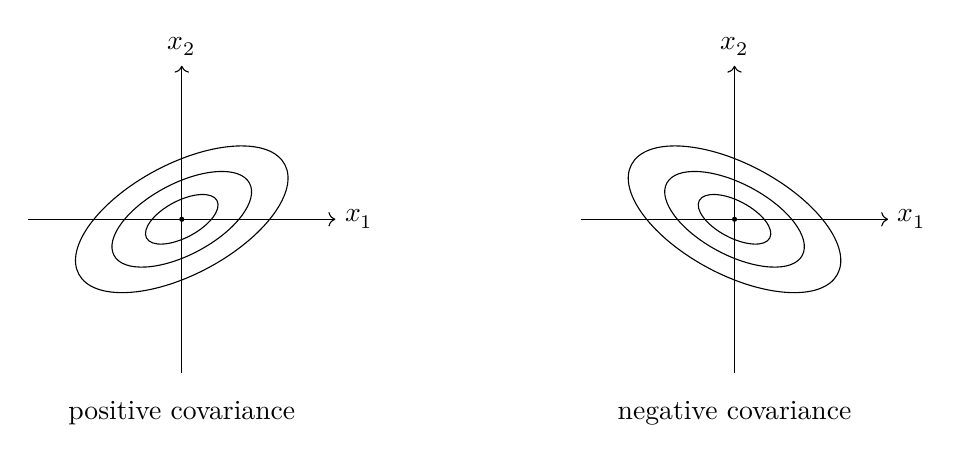
\begin{tikzpicture}[scale=0.78]
    \begin{scope}[xshift=-4.5cm]
        \draw[->] (-2.5,0) -- (2.5,0) node[right] {$x_1$};
        \draw[->] (0,-2.5) -- (0,2.5) node[above] {$x_2$};
        \fill (0,0) circle (1.2pt);
        \draw[rotate around={28:(0,0)}] (0,0) ellipse (1.9 and 0.9);
        \draw[rotate around={28:(0,0)}] (0,0) ellipse (1.25 and 0.58);
        \draw[rotate around={28:(0,0)}] (0,0) ellipse (0.65 and 0.3);
        \node[below] at (0,-2.8) {positive covariance};
    \end{scope}
    \begin{scope}[xshift=4.5cm]
        \draw[->] (-2.5,0) -- (2.5,0) node[right] {$x_1$};
        \draw[->] (0,-2.5) -- (0,2.5) node[above] {$x_2$};
        \fill (0,0) circle (1.2pt);
        \draw[rotate around={-28:(0,0)}] (0,0) ellipse (1.9 and 0.9);
        \draw[rotate around={-28:(0,0)}] (0,0) ellipse (1.25 and 0.58);
        \draw[rotate around={-28:(0,0)}] (0,0) ellipse (0.65 and 0.3);
        \node[below] at (0,-2.8) {negative covariance};
    \end{scope}
\end{tikzpicture}
\end{center}

\begin{example}[Choosing the right distribution]
Orders arrive according to a Poisson process with rate $3$ per minute. What is the probability of exactly $5$ orders in the next $2$ minutes, and what is the probability that the next order arrives after $30$ seconds?
\end{example}

\begin{proof}[Solution]
If arrivals form a Poisson process with rate $3$ per minute, then the number of arrivals in a $2$-minute window has Poisson distribution with parameter
\[
\lambda = 3\times 2 = 6.
\]
Therefore
\[
\mathbb{P}(N=5)=e^{-6}\frac{6^5}{5!}.
\]

The waiting time $T$ until the next arrival is exponential with rate $3$ per minute. Since $30$ seconds is $0.5$ minutes,
\[
\mathbb{P}(T>0.5)=e^{-3\cdot 0.5}=e^{-1.5}.
\]
This example is useful because it highlights the meaning of two closely related laws: Poisson for counts in a window and exponential for waiting times between arrivals.
\end{proof}

\begin{example}[Broken stick triangle probability]
Break a stick of length $1$ at two independent uniformly random points. What is the probability that the three pieces can form a triangle?
\end{example}

\begin{proof}[Solution]
Let the breakpoints be $0<U<V<1$. The three lengths are
\[
U, \qquad V-U, \qquad 1-V.
\]
They form a triangle if and only if no piece has length at least $1/2$. Thus we need
\[
U<\frac12, \qquad V-U<\frac12, \qquad 1-V<\frac12.
\]
Equivalently,
\[
U<\frac12, \qquad V>\frac12, \qquad V<U+\frac12.
\]
The sample space is the triangle $0<U<V<1$, which has area $1/2$. The favorable region is a smaller central triangle with area $1/8$. Therefore
\[
\mathbb{P}(\text{triangle}) = \frac{1/8}{1/2}=\frac14.
\]
So the answer is
\[
\boxed{\frac14}.
\]
\end{proof}

\begin{example}[Expected draw time for an inclusive marriage]
An inclusive marriage is a king together with a queen, with suits arbitrary. A standard deck is thoroughly shuffled, and cards are drawn one by one without replacement. Find the expected number of cards that must be drawn until an inclusive marriage has appeared. Express the answer as an irreducible fraction.
\end{example}

\begin{proof}[Solution]
Let $T$ be the number of cards drawn until we have seen at least one king and at least one queen.

Only the $8$ special cards matter: the $4$ kings and the $4$ queens. Ignore the other $44$ cards for a moment and look only at the special cards in the order they appear. This order is a uniformly random permutation of
\[
K,K,K,K,Q,Q,Q,Q.
\]
Let $J$ be the index of the special card at which the first opposite rank appears. Then $J$ can be $2,3,4$, or $5$.

Its distribution is easy to compute:
\[
\mathbb{P}(J=2)=\frac47,
\]
because after the first special card, $4$ of the remaining $7$ special cards have the opposite rank. Also,
\[
\mathbb{P}(J=3)=\frac37\cdot\frac46=\frac27,
\]
\[
\mathbb{P}(J=4)=\frac37\cdot\frac26\cdot\frac45=\frac4{35},
\]
and
\[
\mathbb{P}(J=5)=\frac37\cdot\frac26\cdot\frac15=\frac1{35}.
\]
Therefore
\[
\E[J]=2\cdot\frac47+3\cdot\frac27+4\cdot\frac4{35}+5\cdot\frac1{35}=\frac{13}{5}.
\]

Now let $S_j$ be the position in the full deck of the $j$th special card. The $44$ non-special cards are split into $9$ gaps around the $8$ special cards, and by symmetry each gap has expected size $44/9$. Hence before the $j$th special card there are, on average, $j\cdot 44/9$ ordinary cards, so
\[
\E[S_j]=j+\frac{44j}{9}=\frac{53j}{9}.
\]

The positions of the $8$ special cards are independent of which of those positions are occupied by kings and which by queens, so $J$ is independent of the sequence $(S_j)$. Since $T=S_J$, we obtain
\[
\E[T]=\E[S_J]=\frac{53}{9}\E[J]=\frac{53}{9}\cdot\frac{13}{5}=\frac{689}{45}.
\]
Thus the expected number of cards needed is
\[
\boxed{\frac{689}{45}}.
\]
\end{proof}

\begin{example}[Linear combination of a bivariate normal]
Let
\[
X=\begin{pmatrix}X_1\\X_2\end{pmatrix}
\sim \mathcal{N}_2\!\left(
\begin{pmatrix}1\\-2\end{pmatrix},
\begin{pmatrix}4&1\\1&9\end{pmatrix}
\right).
\]
Find the distribution of $Y=2X_1-X_2$ and estimate $\mathbb{P}(Y>0)$.
\end{example}

\begin{proof}[Solution]
Write
\[
a=\begin{pmatrix}2\\-1\end{pmatrix}.
\]
Then $Y=a^TX$, and every linear combination of a multivariate normal vector is again normal. Therefore
\[
Y\sim \mathcal{N}(a^T\mu, a^T\Sigma a).
\]
Compute the mean:
\[
a^T\mu = 2\cdot 1 -(-2)=4.
\]
Compute the variance:
\[
a^T\Sigma a
=
\begin{pmatrix}2&-1\end{pmatrix}
\begin{pmatrix}4&1\\1&9\end{pmatrix}
\begin{pmatrix}2\\-1\end{pmatrix}
=21.
\]
Hence
\[
Y\sim \mathcal{N}(4,21).
\]

Standardizing gives
\[
\mathbb{P}(Y>0)=\mathbb{P}\left(Z>\frac{0-4}{\sqrt{21}}\right)=\Phi\left(\frac{4}{\sqrt{21}}\right)\approx 0.809,
\]
where $Z\sim \mathcal{N}(0,1)$.

So the final answer is
\[
\boxed{Y\sim \mathcal{N}(4,21), \qquad \mathbb{P}(Y>0)\approx 0.809.}
\]
\end{proof}

\begin{example}[Mean and variance of an urn under a replace-if-black rule]
A basket holds $m$ black balls and $n$ red balls. At each step a uniformly random ball is drawn; if black it is replaced by a red ball, if red it is put back unchanged. Find $\E[R_k]$ and $\Var(R_k)$, the mean and variance of the number of red balls after $k$ steps, as closed-form expressions (no sums or ellipses).
\end{example}

\begin{proof}[Solution]
Label the $N=m+n$ physical balls; balls never leave the basket, and only the $m$ originally black ones can change color. At each step the drawn label is uniform on $\{1,\dots,N\}$ and independent of the history (returning a red ball does not change the distribution of future draws). So a black ball $i$ has turned red by time $k$ exactly when its label was hit at least once among $k$ i.i.d.\ uniform draws.

Let $X_i$ ($i=1,\dots,m$) indicate that black ball $i$ has been drawn by time $k$, and set $a=\left(\frac{N-1}{N}\right)^{k}$, so $\mathbb{P}(X_i=1)=1-a$. Since $R_k=n+\sum_{i=1}^m X_i$,
\[
\E[R_k]=\boxed{\,n+m\left(1-\left(\frac{N-1}{N}\right)^{k}\right)\,}, \qquad N=m+n.
\]

For the variance, let $b=\left(\frac{N-2}{N}\right)^{k}$ be the probability that two fixed labels are \emph{both} never drawn. By inclusion--exclusion, $\mathbb{P}(X_i=1,X_j=1)=1-2a+b$ for $i\ne j$, so
\[
\mathrm{Cov}(X_i,X_j)=(1-2a+b)-(1-a)^2=b-a^2,
\]
while $\Var(X_i)=a(1-a)$. Summing the $m$ variances and $m(m-1)$ covariance pairs,
\[
\Var(R_k)=ma(1-a)+m(m-1)(b-a^2)=ma+m(m-1)b-m^2a^2,
\]
that is,
\[
\boxed{\,\Var(R_k)=m\left(\frac{N-1}{N}\right)^{k}+m(m-1)\left(\frac{N-2}{N}\right)^{k}-m^2\left(\frac{N-1}{N}\right)^{2k}\,}, \qquad N=m+n.
\]
\end{proof}

\begin{example}[Expected value of the maximum of two independent exponentials]
$X\sim\mathrm{Exp}(1)$ and $Y\sim\mathrm{Exp}(2)$ are independent. Let $Z=\max(X,Y)$. Find $\E[Z]$.
\end{example}

\begin{proof}[Solution]
Use $\max(X,Y)=X+Y-\min(X,Y)$, so $\E[Z]=\E[X]+\E[Y]-\E[\min(X,Y)]$. For independent exponentials with rates $\lambda_1,\lambda_2$, $\min(X,Y)\sim\mathrm{Exp}(\lambda_1+\lambda_2)$ (the minimum of independent exponential ``alarm clocks'' rings at the combined rate). Here $\lambda_1=1,\lambda_2=2$, so $\min(X,Y)\sim\mathrm{Exp}(3)$, with mean $1/3$. Hence
\[
\E[Z]=1+\frac12-\frac13=\boxed{\frac{7}{6}}.
\]
\end{proof}

\begin{example}[Waiting for two different kinds of good news]
Each day, independently, a forum shows a new problem about groups with probability $\tfrac14$, a new problem about rings with probability $\tfrac1{10}$, and nothing new with probability $\tfrac{13}{20}$ (these three outcomes are mutually exclusive and exhaustive). Let $X$ be the smallest number of days after which at least one groups-problem and at least one rings-problem have appeared. Find the distribution of $X$ in closed form.
\end{example}

\begin{proof}[Solution]
Let $p_g=\tfrac14$, $p_r=\tfrac1{10}$, $p_0=\tfrac{13}{20}$ (note $p_g+p_r+p_0=1$). For $\mathbb{P}(X>n)$, use inclusion–exclusion on the events ``no groups-problem in $n$ days'' and ``no rings-problem in $n$ days'':
\[
\mathbb{P}(X>n)=\mathbb{P}(\text{no groups})+\mathbb{P}(\text{no rings})-\mathbb{P}(\text{no groups and no rings}) \quad \text{(in $n$ days)}.
\]
The first two probabilities are $(1-p_g)^n=(3/4)^n$ and $(1-p_r)^n=(9/10)^n$. Since the three daily outcomes are mutually exclusive, ``no groups and no rings'' means every day is the ``nothing'' outcome, with probability $p_0^n=(13/20)^n$. So
\[
\mathbb{P}(X>n)=\left(\frac34\right)^n+\left(\frac9{10}\right)^n-\left(\frac{13}{20}\right)^n.
\]
Then $\mathbb{P}(X=n)=\mathbb{P}(X>n-1)-\mathbb{P}(X>n)$, and each of the three terms telescopes as $c^{n-1}-c^n=c^{n-1}(1-c)$:
\[
\boxed{\mathbb{P}(X=n)=\frac14\left(\frac34\right)^{n-1}+\frac1{10}\left(\frac9{10}\right)^{n-1}-\frac{7}{20}\left(\frac{13}{20}\right)^{n-1}}, \qquad n=1,2,3,\dots
\]
(At $n=1$ this correctly gives $0$, since one day can never supply both a groups- and a rings-problem. At $n=2$ it gives $\tfrac1{20}$, matching the direct check $\mathbb P(X=2)=2p_gp_r=2\cdot\tfrac14\cdot\tfrac1{10}=\tfrac1{20}$: the only way to finish exactly on day $2$ is one day of each type, in either order.)
\end{proof}

\begin{example}[Length of the cycle joining two fixed elements of a random permutation]
For a uniformly random permutation of $\{1,\dots,n\}$, let $X$ be the length of the cycle containing both $1$ and $2$ (and $X=0$ if $1$ and $2$ lie in different cycles). Find the distribution of $X$ and $\E[X]$.
\end{example}

\begin{proof}[Solution]
For $k=2,\dots,n$, count permutations where $1,2$ lie together in a cycle of length exactly $k$: choose the other $k-2$ cycle members from the remaining $n-2$ elements ($\binom{n-2}{k-2}$ ways), arrange all $k$ chosen elements into a single cycle ($(k-1)!$ distinct cyclic arrangements), and permute the other $n-k$ elements freely ($(n-k)!$ ways). Dividing by $n!$,
\[
\mathbb P(X=k)=\frac{\binom{n-2}{k-2}(k-1)!(n-k)!}{n!}=\frac{(n-2)!\,(k-1)!}{(k-2)!\,n!}=\frac{k-1}{n(n-1)}, \qquad k=2,\dots,n.
\]
Summing, $\sum_{k=2}^n\frac{k-1}{n(n-1)}=\frac{1}{n(n-1)}\sum_{j=1}^{n-1}j=\frac{1}{n(n-1)}\cdot\frac{n(n-1)}2=\frac12$, so
\[
\boxed{\mathbb P(X=0)=\frac12, \qquad \mathbb P(X=k)=\frac{k-1}{n(n-1)} \ (k=2,\dots,n)}
\]
(a well-known fact: two fixed elements of a random permutation lie in the same cycle with probability exactly $\tfrac12$, regardless of $n$).

For the mean, $\E[X]=\sum_{k=2}^n k\cdot\frac{k-1}{n(n-1)}=\frac{1}{n(n-1)}\sum_{k=2}^n k(k-1)$. Using the hockey-stick identity $\sum_{k=2}^n\binom k2=\binom{n+1}3$, so $\sum_{k=2}^nk(k-1)=2\binom{n+1}3=\frac{n(n-1)(n+1)}3$, giving
\[
\boxed{\E[X]=\frac{n+1}{3}}.
\]
\end{proof}

\begin{example}[Density of a Laplace–Uniform combination]
$X$ and $Y$ are independent, $X$ has the Laplace density $\tfrac12e^{-|x|}$ and $Y\sim\mathrm{Unif}[1,2]$. Find the density of $Z=X-2Y$.
\end{example}

\begin{proof}[Solution]
Let $W=-2Y$; since $Y\sim\mathrm{Unif}[1,2]$, $W\sim\mathrm{Unif}[-4,-2]$ with density $f_W(w)=\tfrac12$ on $[-4,-2]$. Then $Z=X+W$ is a sum of independent variables, so its density is the convolution
\[
f_Z(z)=\int_{-4}^{-2} \frac12 e^{-|z-w|}\cdot\frac12\,dw = \frac14\int_{-4}^{-2}e^{-|z-w|}\,dw \overset{u=z-w}{=} \frac14\int_{z+2}^{z+4} e^{-|u|}\,du.
\]
Evaluate according to where the window $[z+2,z+4]$ sits relative to $0$:
\begin{itemize}
\item $z\le-4$ (window entirely $\le0$, $e^{-|u|}=e^u$): $\displaystyle\int_{z+2}^{z+4}e^u\,du=e^{z+4}-e^{z+2}=e^z(e^4-e^2)$.
\item $z\ge-2$ (window entirely $\ge0$, $e^{-|u|}=e^{-u}$): $\displaystyle\int_{z+2}^{z+4}e^{-u}\,du=e^{-(z+2)}-e^{-(z+4)}=e^{-z}(e^{-2}-e^{-4})$.
\item $-4<z<-2$ (window straddles $0$): $\displaystyle\int_{z+2}^0e^u\,du+\int_0^{z+4}e^{-u}\,du = (1-e^{z+2})+(1-e^{-(z+4)}) = 2-e^{z+2}-e^{-z-4}$.
\end{itemize}
So
\[
\boxed{f_Z(z)=\begin{cases}
\dfrac{e^4-e^2}{4}\,e^{z}, & z\le-4,\\[2mm]
\dfrac12-\dfrac14e^{z+2}-\dfrac14e^{-z-4}, & -4<z<-2,\\[2mm]
\dfrac{e^{-2}-e^{-4}}{4}\,e^{-z}, & z\ge-2.
\end{cases}}
\]
(One can check this is continuous at $z=-4,-2$ and integrates to $1$ over $\R$, as required of a density.)
\end{proof}

\begin{example}[Catching one of two random trains]
Two trains arrive at a station at independent random times $T_1,T_2\sim\mathrm{Exp}(1)$. A student arrives at time $2$. (a) Find the probability the student can catch at least one train (i.e.\ some $T_i\ge2$). (b) Find the expected waiting time for the nearer catchable train (defined to be $0$ if both trains already came before time $2$).
\end{example}

\begin{proof}[Solution]
\textbf{(a)} $\mathbb P(T_i<2)=1-e^{-2}$ for each $i$, independently, so
\[
\mathbb P(\text{at least one } T_i\ge2) = 1-\mathbb P(T_1<2,T_2<2) = 1-(1-e^{-2})^2 = \boxed{2e^{-2}-e^{-4}}.
\]

\textbf{(b)} Let $W$ be the waiting time. If both $T_1,T_2\ge2$, $W=\min(T_1,T_2)-2$; if exactly one is $\ge2$, $W$ equals that one minus $2$; if both are $<2$, $W=0$. Split the computation into the region where both $T_i\ge2$ and the (symmetric, times $2$) region where exactly one is:
\[
\E[W] = \underbrace{\iint_{t_1,t_2\ge2}(\min(t_1,t_2)-2)e^{-t_1-t_2}\,dt_1dt_2}_{\text{both} \ge 2} + 2\underbrace{\iint_{t_1\ge2,\,t_2<2}(t_1-2)e^{-t_1-t_2}\,dt_1dt_2}_{\text{only } t_1\ge 2}.
\]
For the first integral, substitute $s_i=t_i-2\ge0$: it becomes $e^{-4}\iint_{s_1,s_2\ge0}\min(s_1,s_2)e^{-s_1-s_2}\,ds_1ds_2 = e^{-4}\,\E[\min(S_1,S_2)]$ for $S_1,S_2\sim\mathrm{Exp}(1)$ i.i.d.; since $\min$ of two independent $\mathrm{Exp}(1)$'s is $\mathrm{Exp}(2)$ with mean $\tfrac12$, this is $e^{-4}/2$.

For the second integral, it factors: $\left[\int_2^\infty(t_1-2)e^{-t_1}dt_1\right]\left[\int_0^2e^{-t_2}dt_2\right] = e^{-2}\cdot(1-e^{-2}) = e^{-2}-e^{-4}$ (the first factor substitutes $u=t_1-2$ to get $e^{-2}\int_0^\infty ue^{-u}du=e^{-2}\cdot1$).

Combining,
\[
\E[W] = \frac{e^{-4}}2 + 2(e^{-2}-e^{-4}) = \boxed{2e^{-2}-\frac32e^{-4}}.
\]
\end{proof}

\subsection{Inequalities, Modes of Convergence, and Characteristic Functions}
\textbf{Definitions and formulas.}
\begin{itemize}
    \item Markov's inequality for nonnegative $X$:
    \[
        \mathbb{P}(X\ge a)\le \frac{\E[X]}{a}.
    \]
    \item Chebyshev's inequality:
    \[
        \mathbb{P}(|X-\mu|\ge k\sigma)\le \frac{1}{k^2}.
    \]
    \item Jensen's inequality: if $\varphi$ is convex, then
    \[
        \varphi(\E[X])\le \E[\varphi(X)].
    \]
    \item Borel--Cantelli: if $\sum_n \mathbb{P}(A_n)<\infty$, then only finitely many $A_n$ occur almost surely.
    \item Common convergence notions:
    \begin{itemize}
        \item almost sure: $X_n\to X$ a.s.;
        \item in probability: $\mathbb{P}(|X_n-X|>\varepsilon)\to 0$;
        \item in $L^p$: $\E[|X_n-X|^p]\to 0$;
        \item in distribution: $F_{X_n}(x)\to F_X(x)$ at continuity points of $F_X$.
    \end{itemize}
    \item The weak law says sample means converge in probability; the strong law says they converge almost surely; the central limit theorem describes the \emph{fluctuation scale} around the law-of-large-numbers limit. For i.i.d. $X_i$ with mean $\mu$ and variance $\sigma^2<\infty$,
    \[
        \sqrt{n}\,\frac{\bar X_n-\mu}{\sigma} \Rightarrow \mathcal{N}(0,1).
    \]
    Equivalently, for large $n$,
    \[
        \bar X_n \approx \mathcal{N}\!\left(\mu,\frac{\sigma^2}{n}\right),
        \qquad
        S_n=X_1+\cdots+X_n \approx \mathcal{N}(n\mu,n\sigma^2).
    \]
    For lattice variables such as binomial counts, a continuity correction often improves the approximation.
    \item The characteristic function of $X$ is
    \[
        \varphi_X(t)=\E[e^{itX}].
    \]
    For independent $X,Y$, $\varphi_{X+Y}(t)=\varphi_X(t)\varphi_Y(t)$.
\end{itemize}

\textbf{Standard normal reference curve.} CLT approximations are usually read off after standardizing to the bell curve below.

\begin{center}
\begin{tikzpicture}
\begin{axis}[
    width=0.72\linewidth,
    height=5.2cm,
    domain=-4:4,
    samples=140,
    axis lines=left,
    xlabel={$z$},
    ylabel={density},
    ymin=0,
    ymax=0.43,
    xtick={-2,0,2},
    ytick=\empty,
    clip=false
]
\addplot[thick] {exp(-x^2/2)/sqrt(2*pi)};
\addplot[dashed] coordinates {(-2,0) (-2,0.055)};
\addplot[dashed] coordinates {(2,0) (2,0.055)};
\end{axis}
\end{tikzpicture}
\end{center}

\begin{example}[Chebyshev bound for a sample mean]
Let $X_1,\dots,X_{400}$ be i.i.d. with mean $0$ and variance $1$. Give an upper bound on
\[
\mathbb{P}\left(\left|\frac{1}{400}\sum_{i=1}^{400}X_i\right|>0.1\right)
\]
using Chebyshev's inequality.
\end{example}

\begin{proof}[Solution]
Let $\bar X_{400}=\frac{1}{400}\sum_{i=1}^{400}X_i$. Then
\[
\E[\bar X_{400}]=0, \qquad \Var(\bar X_{400})=\frac{1}{400^2}\cdot 400 = \frac{1}{400}.
\]
By Chebyshev,
\[
\mathbb{P}(|\bar X_{400}|>0.1) \le \frac{\Var(\bar X_{400})}{0.1^2} = \frac{1/400}{0.01} = \frac14.
\]
Hence
\[
\boxed{\mathbb{P}(|\bar X_{400}|>0.1)\le \frac14}.
\]
This is conservative but completely distribution-free.
\end{proof}

\begin{example}[Central limit approximation to a binomial count]
A fair coin is tossed $400$ times. Estimate
\[
\mathbb{P}(180\le X\le 220),
\]
where $X$ is the number of heads.
\end{example}

\begin{proof}[Solution]
Here
\[
X\sim \mathrm{Bin}(400,1/2),
\qquad
\mu=np=200,
\qquad
\sigma=\sqrt{np(1-p)}=10.
\]
By the central limit theorem, $X$ is well approximated by a normal variable with the same mean and variance. Using a continuity correction,
\[
\mathbb{P}(180\le X\le 220)
\approx
\mathbb{P}(179.5\le Y\le 220.5),
\]
where $Y\sim \mathcal{N}(200,100)$.

Standardize:
\[
\mathbb{P}(179.5\le Y\le 220.5)
=
\mathbb{P}\left(\frac{179.5-200}{10}\le Z\le \frac{220.5-200}{10}\right)
=
\mathbb{P}(-2.05\le Z\le 2.05),
\]
where $Z\sim \mathcal{N}(0,1)$.
Therefore
\[
\mathbb{P}(180\le X\le 220)
\approx 2\Phi(2.05)-1
\approx 0.9596.
\]
So the CLT estimate is
\[
\boxed{\mathbb{P}(180\le X\le 220)\approx 0.960.}
\]
\end{proof}

\begin{example}[A random increment process with shrinking step size]
Assume $x_3>0$ is fixed. For each $t\ge 3$, the process adds the current increment $x_t$ to $V$, and then independently updates the next increment by
\[
x_{t+1}=
\begin{cases}
x_t/2, & \text{with probability } 2/t,\\
x_t, & \text{with probability } 1-2/t.
\end{cases}
\]
What is the probability that $V_t\to\infty$ as $t\to\infty$?
\end{example}

\begin{proof}[Solution]
Let $I_t$ be the indicator that a halving occurs at time $t$, and let
\[
N_n=\sum_{t=3}^n I_t
\]
be the total number of halvings up to time $n$. Then
\[
x_n = x_3\,2^{-N_{n-1}}.
\]
Since the halving decisions are independent and $\mathbb{P}(I_t=1)=2/t$,
\[
\E[N_n]=\sum_{t=3}^n \frac{2}{t}=2\log n + O(1).
\]
By the strong law for sums of independent Bernoulli variables with varying parameters,
\[
N_n = 2\log n + o(\log n) \qquad \text{almost surely}.
\]
Therefore
\[
x_n = x_3\exp\bigl(- (\log 2)N_{n-1}\bigr)
= n^{-2\log 2 + o(1)} \qquad \text{almost surely}.
\]
Now
\[
2\log 2 \approx 1.386 > 1,
\]
so almost surely the series $\sum_n x_n$ behaves like a $p$-series with exponent strictly larger than $1$. Hence
\[
\sum_{n=3}^{\infty} x_n < \infty \qquad \text{almost surely}.
\]
But $V_t$ is obtained by summing these increments, so $V_t$ converges to a finite random limit almost surely. Consequently,
\[
\boxed{\mathbb{P}(V_t\to\infty)=0}.
\]

This is a useful warning example: even though the expected number of halvings by time $n$ is only logarithmic, that is still enough to make the typical increment decay faster than $1/n$, so the cumulative growth stays finite almost surely.
\end{proof}

\begin{example}[A negative-binomial tail sum via the CLT]
Find
\[
\lim_{n\to\infty}\sum_{k=n}^{5n} \binom{k-1}{n-1}\left(\frac15\right)^n\left(\frac45\right)^{k-n}.
\]
\end{example}

\begin{proof}[Solution]
The summand $\binom{k-1}{n-1}p^n(1-p)^{k-n}$ (with $p=\tfrac15$) is exactly $\mathbb{P}(N=k)$ where $N$ is the trial number of the $n$-th success in i.i.d.\ $\mathrm{Bernoulli}(p)$ trials: the $n$-th success lands on trial $k$ iff exactly $n-1$ of the first $k-1$ trials succeed (probability $\binom{k-1}{n-1}p^{n-1}(1-p)^{k-n}$) and trial $k$ itself succeeds (probability $p$). So the sum equals $\mathbb{P}(n\le N\le 5n)$ for $N\sim\mathrm{NegBinomial}(n,p)$.

Write $N=\sum_{i=1}^n G_i$ where $G_i$ are i.i.d.\ $\mathrm{Geometric}(p)$ (number of trials to get the $i$-th success after the $(i-1)$-th), each with $\E[G_i]=1/p=5$ and $\Var(G_i)=(1-p)/p^2=20$. So $\E[N]=5n$ and $\Var(N)=20n$, giving standard deviation $\sqrt{20n}=\Theta(\sqrt n)$.

\emph{Lower tail.} $n$ is $4n$ below the mean $5n$, which is $\Theta(n)\gg\Theta(\sqrt n)$, so by Chebyshev,
\[
\mathbb{P}(N<n)\le\mathbb{P}(|N-5n|>4n)\le\frac{\Var(N)}{(4n)^2}=\frac{20n}{16n^2}=\frac{5}{4n}\xrightarrow[n\to\infty]{}0.
\]

\emph{Upper tail at the mean.} By the Central Limit Theorem, $\dfrac{N-5n}{\sqrt{20n}}$ converges in distribution to a standard normal, so
\[
\mathbb{P}(N\le5n)=\mathbb{P}\!\left(\frac{N-5n}{\sqrt{20n}}\le0\right)\xrightarrow[n\to\infty]{}\Phi(0)=\frac12.
\]

Combining, $\mathbb{P}(n\le N\le5n)=\mathbb{P}(N\le5n)-\mathbb{P}(N<n)\to\tfrac12-0$, so
\[
\boxed{\frac12}.
\]
(Direct numerical summation confirms the convergence: the partial sum is about $0.526$ at $n=50$, $0.513$ at $n=200$, and $0.501$ at $n=20{,}000$.)
\end{proof}

\begin{example}[A Gaussian tail series with a log-log correction]
Let $\xi_1,\xi_2,\dots$ each have the standard normal distribution. Does $\displaystyle\sum_{n=1}^\infty \mathbb P\!\left(\xi_n>\sqrt{2\ln n+2\ln\ln n}\right)$ converge?
\end{example}

\begin{proof}[Solution]
Use the standard Gaussian tail bound $\mathbb P(\xi>x)\le \varphi(x)/x$ for $x>0$, where $\varphi(x)=\frac1{\sqrt{2\pi}}e^{-x^2/2}$. Let $x_n=\sqrt{2\ln n+2\ln\ln n}$ (defined for $n\ge3$, where $\ln\ln n\ge0$). Then
\[
x_n^2 = 2\ln n+2\ln\ln n \quad\Longrightarrow\quad e^{-x_n^2/2}=e^{-\ln n-\ln\ln n}=\frac1{n\ln n}.
\]
Also $x_n\ge\sqrt{2\ln n}$ (dropping the nonnegative $2\ln\ln n$ term), so
\[
\mathbb P(\xi_n>x_n)\le \frac{1}{\sqrt{2\pi}\,x_n}\cdot\frac1{n\ln n} \le \frac{1}{\sqrt{2\pi}\cdot\sqrt{2\ln n}\cdot n\ln n} = \frac{1}{2\sqrt\pi}\cdot\frac{1}{n(\ln n)^{3/2}}.
\]
The series $\sum_{n\ge3} \dfrac1{n(\ln n)^{3/2}}$ converges (the standard $\sum 1/(n(\ln n)^p)$ test, e.g.\ via the integral test on $\int_3^\infty dx/(x(\ln x)^p)$, converges exactly when $p>1$, and here $p=3/2>1$). By comparison, so does the original series (the finitely many small-$n$ terms don't affect convergence):
\[
\boxed{\text{yes, the series converges}}
\]
(numerically, the partial sums stabilize quickly: about $0.548$ by $n=10^6$ and $0.551$ by $n\approx2\times10^6$, consistent with a finite limit).
\end{proof}

\subsection{Markov Chains and First-Step Analysis}
\textbf{Definitions and formulas.}
\begin{itemize}
    \item A Markov chain has transition matrix $P=(p_{ij})$, where
    \[
        p_{ij}=\mathbb{P}(X_{n+1}=j\mid X_n=i).
    \]
    Each row of $P$ sums to $1$. The key modeling step is to choose the state so that, once the current state is known, the future no longer depends on the earlier history. In interview problems, the hard part is usually not matrix algebra but selecting the right state description.
    \item A distribution $\pi$ is stationary if $\pi P=\pi$. This means that if the chain starts with distribution $\pi$, then after one step it still has distribution $\pi$. For ergodic finite chains, this is the long-run equilibrium law.
    \item In a finite irreducible and aperiodic chain, the stationary distribution is unique and the chain converges to it regardless of the starting state. Irreducible means every state can eventually reach every other state, and aperiodic means the chain is not trapped in a rigid cycle length.
    \item Hitting probabilities are handled by the same one-step idea. If
    \[
        q_i=\mathbb{P}_i(\tau_A<\tau_B),
    \]
    then the boundary conditions are
    \[
        q_i=1 \text{ for } i\in A,
        \qquad
        q_i=0 \text{ for } i\in B,
    \]
    and for all other states,
    \[
        q_i=\sum_j p_{ij}q_j.
    \]
    There is no extra $1$ here because we are computing a probability, not a time. We simply average the future success probability over the next state.
    \item Expected hitting times are often solved by \emph{first-step analysis}: condition on the next move and write a recursion.
    \item If $\tau_A$ is the first hitting time of a set $A$, then the expected hitting times satisfy
    \[
        h_i=0 \text{ for } i\in A,
        \qquad
        h_i = 1+\sum_j p_{ij}h_j \text{ for } i\notin A.
    \]
    The extra $1$ is the step you take immediately before landing in the next state.
    \item Absorbing-state problems reduce to linear systems. Once you assign one variable to each transient state, the recursion from first-step analysis produces one linear equation per unknown.
    \item For an absorbing Markov chain with block form
    \[
        P=\begin{pmatrix}Q&R\\0&I\end{pmatrix},
    \]
    the matrix $Q$ describes transitions among transient states, $R$ describes jumps from transient states to absorbing states, and the fundamental matrix is $N=(I-Q)^{-1}$. The entry $N_{ij}$ is the expected number of visits to transient state $j$ when starting from transient state $i$, before absorption occurs. Summing across a row gives the expected absorption time, so $N\mathbf{1}$ gives expected absorption times from transient states.
\end{itemize}

\textbf{Transition-graph picture.} The matrix and the directed graph contain the same information: draw one node per state and an arrow $i\to j$ labeled by $p_{ij}$ whenever $p_{ij}>0$. For the random walk example below, the chain can be visualized as follows.

\begin{center}
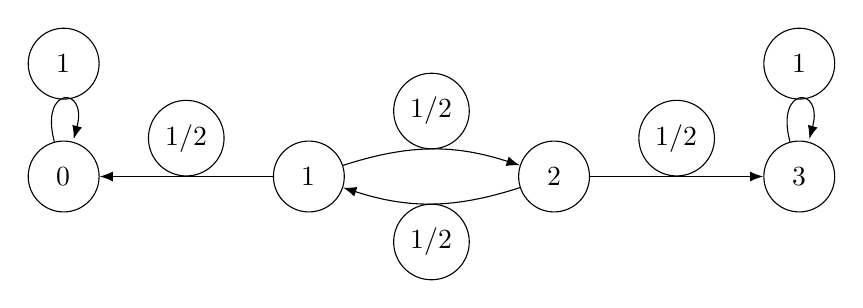
\begin{tikzpicture}[>=Latex, node distance=2.2cm, every node/.style={draw, circle, minimum size=9mm}]
    \node (0) {$0$};
    \node (1) [right=of 0] {$1$};
    \node (2) [right=of 1] {$2$};
    \node (3) [right=of 2] {$3$};

    \draw[->] (1) to[bend left=18] node[above] {$1/2$} (2);
    \draw[->] (2) to[bend left=18] node[below] {$1/2$} (1);
    \draw[->] (1) -- node[above] {$1/2$} (0);
    \draw[->] (2) -- node[above] {$1/2$} (3);
    \draw[->] (0) edge[loop above] node {$1$} (0);
    \draw[->] (3) edge[loop above] node {$1$} (3);
\end{tikzpicture}
\end{center}

The absorbing states $0$ and $3$ have self-loops of probability $1$. States $1$ and $2$ are transient because, once the walk enters $0$ or $3$, it never returns.

\textbf{Practical workflow.}
\begin{enumerate}
    \item Choose states that retain exactly the information that still matters for the future.
    \item Write one equation per nonterminal state by conditioning on the next step.
    \item Put boundary values on terminal or absorbing states.
    \item Solve the resulting linear system.
    \item Read off the quantity corresponding to the actual starting state.
\end{enumerate}

In interview practice there are three recurring templates:
\begin{itemize}
    \item If you are asked for a probability of eventually hitting one target before another, define $q_i$ and use $q_i=\sum_j p_{ij}q_j$.
    \item If you are asked for an expected waiting time, define $h_i$ and use $h_i=1+\sum_j p_{ij}h_j$.
    \item If the process only depends on a small memory of the past, compress the past into a few states. The two-sixes example below is exactly of this type.
\end{itemize}

\begin{example}[Expected rolls until two consecutive sixes]
You roll a fair six-sided die repeatedly. What is the expected number of rolls until two consecutive sixes appear?
\end{example}

\begin{proof}[Solution]
Use two states, chosen so that the future depends only on whether we are currently carrying a trailing $6$:
\begin{itemize}
    \item $E_0$: expected additional rolls when we do \emph{not} currently have a trailing $6$;
    \item $E_1$: expected additional rolls when the previous roll was a $6$, so one more $6$ finishes the game.
\end{itemize}
At the start of the experiment no roll has happened yet, so we are in state $E_0$, not $E_1$. That is why the answer to the problem will be $E_0$.

This is the standard state-compression trick: the whole past sequence of rolls is irrelevant except for one bit of information, namely whether the most recent roll was a $6$.

From state $E_0$, one roll occurs, and then with probability $5/6$ we remain in $E_0$, while with probability $1/6$ we move to $E_1$:
\[
E_0 = 1 + \frac{5}{6}E_0 + \frac{1}{6}E_1.
\]
From state $E_1$, one roll occurs. With probability $1/6$ we finish, and with probability $5/6$ we return to $E_0$:
\[
E_1 = 1 + \frac{5}{6}E_0.
\]
The first equation simplifies to
\[
E_0 = 6 + E_1.
\]
Substitute into the second:
\[
E_1 = 1 + \frac{5}{6}(6+E_1)=6+\frac{5}{6}E_1.
\]
Thus
\[
\frac{1}{6}E_1=6 \quad \Longrightarrow \quad E_1=36,
\]
and therefore
\[
E_0=6+36=42.
\]
Because the chain starts in state $E_0$, the expected number of rolls asked for in the problem is
\[
\boxed{42}.
\]
The structure is worth remembering: one equation per nonterminal state, one immediate step cost, and then an average over the next states.
\end{proof}

\begin{example}[Absorption on a short random walk]
A particle moves on the states $0,1,2,3$. States $0$ and $3$ are absorbing. From states $1$ and $2$, the particle moves left or right with probability $1/2$ each. If the chain starts at state $1$, find the probability of being absorbed at $3$ and the expected time to absorption.
\end{example}

\begin{proof}[Solution]
Let $p_i$ be the probability, starting from state $i$, of hitting $3$ before $0$. Then
\[
p_0=0,
\qquad
p_3=1,
\]
and by first-step analysis,
\[
p_1=\frac{p_0+p_2}{2}=\frac{p_2}{2},
\qquad
p_2=\frac{p_1+p_3}{2}=\frac{p_1+1}{2}.
\]
Substituting the first equation into the second gives
\[
p_2=\frac{p_2/2+1}{2},
\]
so $4p_2=p_2+2$, hence $p_2=\frac23$ and therefore
\[
p_1=\frac13.
\]
Thus the probability of absorption at $3$ when starting from $1$ is
\[
\boxed{\frac13}.
\]

This is the hitting-probability template in its purest form: no extra $1$ appears because we are not counting time, only eventual success.

Now let $e_i$ be the expected time to absorption starting from state $i$. Then
\[
e_0=e_3=0,
\]
and
\[
e_1=1+\frac{e_0+e_2}{2}=1+\frac{e_2}{2},
\qquad
e_2=1+\frac{e_1+e_3}{2}=1+\frac{e_1}{2}.
\]
Substitute the second equation into the first:
\[
e_1=1+\frac{1+e_1/2}{2}=\frac32+\frac{e_1}{4}.
\]
Hence
\[
\frac{3e_1}{4}=\frac32,
\qquad
e_1=2.
\]
So the expected time to absorption is
\[
\boxed{2}.
\]
Here the extra $1$ appears because one step is spent immediately, regardless of which direction the walk takes next.
\end{proof}

\begin{example}[Expected hitting time in a small portal maze]
A maze has $6$ rooms connected by two-way portals as follows: room $1$ connects to $2,3$; room $2$ connects to $1,3,4,6$; room $3$ connects to $1,2,5,6$; room $4$ connects to $2,5,6$; room $5$ connects to $3,4,6$; room $6$ connects to $2,3,4,5$. Starting in room $1$, at each step you jump through a uniformly random portal from your current room (including possibly back the way you came). Find the expected number of jumps to first reach room $6$.
\end{example}

\begin{proof}[Solution]
Let $h_i$ be the expected number of jumps to reach room $6$ starting from room $i$ ($h_6=0$). First-step analysis gives, for each room $i\neq6$ with degree $d_i$ and neighbors $N(i)$,
\[
h_i = 1+\frac1{d_i}\sum_{j\in N(i)} h_j.
\]
The degrees here are $d_1=2$, $d_2=d_3=d_6=4$, $d_4=d_5=3$, giving the system
\[
\begin{aligned}
h_1 &= 1+\tfrac12(h_2+h_3), \\
h_2 &= 1+\tfrac14(h_1+h_3+h_4), \\
h_3 &= 1+\tfrac14(h_1+h_2+h_5), \\
h_4 &= 1+\tfrac13(h_2+h_5), \\
h_5 &= 1+\tfrac13(h_3+h_4).
\end{aligned}
\]
By the left-right symmetry of the maze (swapping $2\leftrightarrow3$, $4\leftrightarrow5$ preserves all the adjacencies), $h_2=h_3$ and $h_4=h_5$; substituting collapses the system to two equations in $h_2,h_4$ (with $h_1=1+h_2$ from the first equation):
\[
h_2 = 1+\tfrac14\big((1+h_2)+h_2+h_4\big), \qquad h_4=1+\tfrac13(h_2+h_4).
\]
The second equation gives $\tfrac23h_4=1+\tfrac13h_2$, i.e.\ $h_4=\tfrac32+\tfrac12h_2$. Substituting into the first: $h_2=1+\tfrac14\big(1+2h_2+\tfrac32+\tfrac12h_2\big)=1+\tfrac14\big(\tfrac52+\tfrac52h_2\big)=\tfrac{13}8+\tfrac58h_2$, so $\tfrac38h_2=\tfrac{13}8$, giving $h_2=\tfrac{13}3$, hence $h_4=\tfrac32+\tfrac16\cdot13=\tfrac{11}3$ and
\[
h_1 = 1+h_2 = 1+\frac{13}3=\boxed{\frac{16}{3}}.
\]
(A direct Monte Carlo simulation of the random walk confirms this: the sample mean over $2$ million runs is about $5.337$, matching $16/3\approx5.333$.)
\end{proof}

\section{Algorithm Design}
Quant interviews frequently include short algorithmic problems that reward recognizing a classical pattern — a monotonic stack, a sliding window, a divide-and-conquer trick — over brute force.

\begin{example}[Nearest right element at least double, in $O(n\log n)$]
Given a real array $A[1..n]$, design an algorithm that, for every index $i$, finds the smallest index $j>i$ with $A[j]\ge 2A[i]$ (or reports that none exists), using $O(n\log n)$ time and $O(n)$ extra space.
\end{example}

\begin{proof}[Solution]
\textbf{A domination principle.} Scan the array from right to left, maintaining a stack of surviving candidates. Say index $j_2$ is \emph{dominated} by a nearer index $j_1<j_2$ if $A[j_1]\ge A[j_2]$. A dominated candidate is useless: for any future (further left) query $i$, whenever $A[j_2]\ge 2A[i]$ we also have $A[j_1]\ge A[j_2]\ge2A[i]$, and $j_1$ is strictly closer, so $j_2$ can never be the nearest qualifying index once $j_1$ exists. Notably, this domination argument does not depend on the multiplier $2$; it only uses $A[j_1]\ge A[j_2]$.

\textbf{Maintaining the stack.} Process $i=n,n-1,\dots,1$. Before pushing $i$, pop every index currently on top of the stack with value $\le A[i]$ (those are now dominated by $i$), then push $i$. Each index is pushed and popped at most once, so stack maintenance costs $O(n)$ total.

\textbf{Why the stack is sorted.} Whenever an element is pushed, everything weaker has just been popped, so values strictly increase from the bottom of the stack toward the top — equivalently, reading from the top (nearest to the current scan position) down to the bottom (farthest), values are non-decreasing. So at every moment the live stack is a sequence sorted by value, in which position along the stack corresponds monotonically to distance from the current pointer.

\textbf{Answering a query.} For index $i$ we want the surviving candidate closest to the top with value $\ge2A[i]$. Because the stack is sorted by value from top (smallest) to bottom (largest), the qualifying candidates form a contiguous block at the bottom, and the nearest one is found by \emph{binary search} on the stack (kept as an array) for the threshold $2A[i]$: $O(\log n)$ per query.

\textbf{Complexity.} Maintenance is $O(n)$ amortized; each of the $n$ queries costs $O(\log n)$ via binary search on the array-backed stack; total time is $O(n\log n)$, and the stack never holds more than $n$ indices, so space is $O(n)$ — matching the required bounds exactly. (A plain monotonic stack alone, without the binary search, solves the classical ``next strictly greater element'' problem in $O(n)$; the extra $\log n$ factor here is exactly the cost of the per-query threshold search that the ``at least double'' condition forces.)
\end{proof}

\begin{example}[Sorting a quadratic image of a sorted array, in linear time]
Given a real array $A[1..n]$ sorted in increasing order and real numbers $p,q,r$, produce an array $B[1..n]$ consisting of the values $px^2+qx+r$ for $x\in A$, also sorted in increasing order, using $O(n)$ time and $O(n)$ extra space.
\end{example}

\begin{proof}[Solution]
If $p=0$, $f(x)=qx+r$ is monotonic: copy $A$ through $f$ in order if $q\ge0$, or in reverse order if $q<0$ — $O(n)$.

If $p\neq0$, $f(x)=px^2+qx+r$ is a parabola with vertex at $x_0=-q/(2p)$, monotonic on each side of $x_0$. Since $A$ is sorted, binary search for $x_0$ in $A$ in $O(\log n)$ to split it into $A_{\text{left}}$ (entries $<x_0$) and $A_{\text{right}}$ (entries $\ge x_0$). On one side of $x_0$, $f$ is increasing as $x$ increases; on the other, decreasing — which is which depends on the sign of $p$:
\begin{itemize}
\item $p>0$ (upward parabola): $f$ decreases toward $x_0$ from the left and increases away from it on the right. So $f(A_{\text{left}})$ read in \emph{reverse} order is increasing, and $f(A_{\text{right}})$ read in its original order is already increasing.
\item $p<0$ (downward parabola): the roles swap — $f(A_{\text{left}})$ in its original order is increasing, and $f(A_{\text{right}})$ read in reverse is increasing.
\end{itemize}
Either way, this produces two increasing sequences of total length $n$ in $O(n)$ time. Merge them with the standard two-pointer merge step from merge sort — compare the fronts of each sequence, output the smaller, advance that pointer — in $O(n)$ time and $O(n)$ auxiliary space for the output. The result $B$ is $A$'s image under $f$, fully sorted, using $O(n)$ time (one binary search plus two linear passes) and $O(n)$ space, as required.
\end{proof}

\begin{example}[Largest multiple of $3$ from an array of digits, in $O(n)$ time and $O(1)$ space]
Given an array $A[1..n]$ of digits $0$–$9$, design an algorithm that finds the largest natural number divisible by $3$ that can be formed from (a subset of) the digits of $A$, using $O(n)$ time and $O(1)$ extra space.
\end{example}

\begin{proof}[Solution]
A number is divisible by $3$ iff its digit sum is; and for a fixed multiset of digits, the largest number they form is obtained by arranging them in decreasing order. So the problem reduces to: keep a multiset of digits with digit-sum divisible by $3$, discarding as few (and as small) digits as possible, then output largest-to-smallest.

\textbf{Counting pass.} Scan $A$ once, maintaining a count array $\mathrm{cnt}[0..9]$ (fixed size $10$, so $O(1)$ space) and the running digit sum; this is $O(n)$ time. Let $r=(\text{digit sum})\bmod 3$.

\textbf{Fixing the residue.} If $r=0$, keep every digit. If $r=1$, either discard one digit $\equiv1\pmod3$ (i.e.\ a $1,4,$ or $7$) — choosing the \emph{smallest} such digit value present, to sacrifice as little as possible — or, if no digit $\equiv1\pmod3$ is present at all, discard two digits $\equiv2\pmod3$ (i.e.\ from $2,5,8$; since $2+2\equiv1$), again preferring the smallest available. The case $r=2$ is symmetric: discard one digit $\equiv2\pmod3$, or if none exists, two digits $\equiv1\pmod3$. Each of these adjustments only touches the $10$-entry count array, so it costs $O(1)$ time regardless of $n$.

\textbf{Output.} If every digit was discarded (or only zeros remain), the answer is $0$. Otherwise emit $\mathrm{cnt}[9]$ nines, then $\mathrm{cnt}[8]$ eights, \dots, down to $\mathrm{cnt}[0]$ zeros — a single $O(n)$ pass that reproduces the largest arrangement of the surviving digits.

Total cost: one $O(n)$ counting pass, $O(1)$ work to decide what to discard, and one $O(n)$ output pass — $O(n)$ time, $O(1)$ extra space (the count array has fixed size $10$, independent of $n$).
\end{proof}

\begin{example}[Detecting a $k$-cycle in a permutation given as two arrays]
A permutation $\sigma$ of $\{1,\dots,n\}$ is given by two arrays $a[1..n]$, $b[1..n]$, each containing every value $1,\dots,n$ exactly once, with $b[i]=\sigma(a[i])$ for every $i$ (so $\sigma$ is defined only implicitly — there is no array with $\sigma(i)$ at position $i$). Design an algorithm that decides whether $\sigma$ has a cycle of length exactly $k$ (a fixed constant), using $O(n^2)$ operations and $O(1)$ extra space; the arrays may be modified.
\end{example}

\begin{proof}[Solution]
The obstacle is that $\sigma(x)$ isn't directly indexable: to find it we must locate $x$ in array $a$ and read off the matching entry of $b$.

\textbf{Step 1: put $\sigma$ into direct form, in place.} For $i=1,\dots,n$: scan $a[i..n]$ for the position $j$ with $a[j]=i$ (a linear scan, $O(n)$ per $i$), then swap $(a[i],b[i])\leftrightarrow(a[j],b[j])$ (swapping both arrays' entries together, keeping the pairing $b[\cdot]=\sigma(a[\cdot])$ intact). After this pass, $a[i]=i$ for every $i$, so $b[i]=\sigma(i)$ directly: $b$ is now $\sigma$ in standard array form. This costs $O(n)$ work per index, $O(n^2)$ total, and only a constant number of temporary variables for the swaps — $O(1)$ extra space.

\textbf{Step 2: check for a $k$-cycle.} For each starting point $s=1,\dots,n$, trace $s,\ b[s],\ b[b[s]],\dots$ for exactly $k$ steps, checking along the way that it does not return to $s$ before step $k$ (to rule out a shorter cycle whose length merely divides $k$) and that it \emph{does} return to $s$ at step $k$ exactly. Since $k$ is a constant, each trace costs $O(k)=O(1)$, and there are $n$ starting points, so this phase is $O(n)$.

The dominant cost is the $O(n^2)$ in-place linear-search sort of Step 1 (a simple selection-sort-style pass — an $O(n\log n)$ or even $O(n)$ in-place rearrangement is possible with more care, e.g.\ by following $a$'s own cycles to place each value directly, but $O(n^2)$ already meets the stated bound). Total: $O(n^2)$ time, $O(1)$ extra space.
\end{proof}

\begin{example}[Finding all saddle entries of a matrix in one pass per element]
Call an entry of an $n\times m$ matrix (all entries distinct) a \emph{saddle} if it is the largest in its row and smallest in its column, or the smallest in its row and largest in its column. Design an algorithm that finds all saddles using $O(nm)$ operations, $O(n+m)$ memory, and accesses each entry $A[i][j]$ at most once (it becomes unreadable immediately after).
\end{example}

\begin{proof}[Solution]
The difficulty: knowing whether $A[i][j]$ is a row-extreme requires seeing all of row $i$, and knowing whether it's a column-extreme requires seeing all of column $j$ — but each entry may be read only once, so we cannot revisit $A[i][j]$ after the fact to compare it against a later-completed row or column summary.

\textbf{Single sweep.} Read the matrix once, in any fixed order (e.g.\ row by row). Maintain running arrays $\mathrm{rowMax}[i],\mathrm{rowArgmax}[i],\mathrm{rowMin}[i],\mathrm{rowArgmin}[i]$ for $i=1,\dots,n$ (size $O(n)$) and $\mathrm{colMax}[j],\mathrm{colArgmax}[j],\mathrm{colMin}[j],\mathrm{colArgmin}[j]$ for $j=1,\dots,m$ (size $O(m)$), updating them in $O(1)$ as each entry is read for the first and only time. After the sweep, every one of these $8(n+m)$ numbers is a true global row/column extreme (and its location), even though the matrix entries themselves are no longer accessible.

\textbf{Recovering the saddles without re-reading $A$.} A row-max-and-column-min saddle must sit at $(i,j)$ with $j=\mathrm{rowArgmax}[i]$ (so $A[i][j]$ really is row $i$'s maximum) \emph{and} $i=\mathrm{colArgmin}[j]$ (so it's also column $j$'s minimum) — both conditions are checkable purely from the stored index arrays, no matrix access needed. For each row $i$ there is exactly one candidate column $j=\mathrm{rowArgmax}[i]$ to check, in $O(1)$, so this pass costs $O(n)$. Symmetrically, checking $j=\mathrm{rowArgmin}[i]$ against $i=\mathrm{colArgmax}[j]$ for each row finds all row-min-and-column-max saddles, another $O(n)$.

\textbf{Complexity.} The sweep costs $O(nm)$ (each of the $nm$ entries touched exactly once, $O(1)$ work each); the two candidate-checking passes cost $O(n)$ total; the stored arrays use $O(n+m)$ memory. Every entry of $A$ is read exactly once, as required, and every saddle is found (and nothing else is reported, since both defining conditions are checked exactly).
\end{proof}

\section*{How to Use This Guide Efficiently}
\begin{itemize}
    \item Memorize formulas only after you understand where they come from.
    \item When a problem looks hard, first classify it: parity, conditioning, asymptotics, optimization, or linear structure.
    \item In an interview, write down the state variables explicitly. A correct state definition is usually half of the solution.
    \item For revision, cover the solutions and try to reproduce them from the definitions and formulas alone.
\end{itemize}

\end{document}
